\documentclass[twoside]{book}

% Packages required by doxygen
\usepackage{fixltx2e}
\usepackage{calc}
\usepackage{doxygen}
\usepackage[export]{adjustbox} % also loads graphicx
\usepackage{graphicx}
\usepackage[utf8]{inputenc}
\usepackage{makeidx}
\usepackage{multicol}
\usepackage{multirow}
\PassOptionsToPackage{warn}{textcomp}
\usepackage{textcomp}
\usepackage[nointegrals]{wasysym}
\usepackage[table]{xcolor}

% Font selection
\usepackage[T1]{fontenc}
\usepackage[scaled=.90]{helvet}
\usepackage{courier}
\usepackage{amssymb}
\usepackage{sectsty}
\renewcommand{\familydefault}{\sfdefault}
\allsectionsfont{%
  \fontseries{bc}\selectfont%
  \color{darkgray}%
}
\renewcommand{\DoxyLabelFont}{%
  \fontseries{bc}\selectfont%
  \color{darkgray}%
}
\newcommand{\+}{\discretionary{\mbox{\scriptsize$\hookleftarrow$}}{}{}}

% Page & text layout
\usepackage{geometry}
\geometry{%
  a4paper,%
  top=2.5cm,%
  bottom=2.5cm,%
  left=2.5cm,%
  right=2.5cm%
}
\tolerance=750
\hfuzz=15pt
\hbadness=750
\setlength{\emergencystretch}{15pt}
\setlength{\parindent}{0cm}
\setlength{\parskip}{0.2cm}
\makeatletter
\renewcommand{\paragraph}{%
  \@startsection{paragraph}{4}{0ex}{-1.0ex}{1.0ex}{%
    \normalfont\normalsize\bfseries\SS@parafont%
  }%
}
\renewcommand{\subparagraph}{%
  \@startsection{subparagraph}{5}{0ex}{-1.0ex}{1.0ex}{%
    \normalfont\normalsize\bfseries\SS@subparafont%
  }%
}
\makeatother

% Headers & footers
\usepackage{fancyhdr}
\pagestyle{fancyplain}
\fancyhead[LE]{\fancyplain{}{\bfseries\thepage}}
\fancyhead[CE]{\fancyplain{}{}}
\fancyhead[RE]{\fancyplain{}{\bfseries\leftmark}}
\fancyhead[LO]{\fancyplain{}{\bfseries\rightmark}}
\fancyhead[CO]{\fancyplain{}{}}
\fancyhead[RO]{\fancyplain{}{\bfseries\thepage}}
\fancyfoot[LE]{\fancyplain{}{}}
\fancyfoot[CE]{\fancyplain{}{}}
\fancyfoot[RE]{\fancyplain{}{\bfseries\scriptsize Generated on Thu Mar 10 2016 11\+:32\+:56 for Guacho 3\+D by Doxygen }}
\fancyfoot[LO]{\fancyplain{}{\bfseries\scriptsize Generated on Thu Mar 10 2016 11\+:32\+:56 for Guacho 3\+D by Doxygen }}
\fancyfoot[CO]{\fancyplain{}{}}
\fancyfoot[RO]{\fancyplain{}{}}
\renewcommand{\footrulewidth}{0.4pt}
\renewcommand{\chaptermark}[1]{%
  \markboth{#1}{}%
}
\renewcommand{\sectionmark}[1]{%
  \markright{\thesection\ #1}%
}

% Indices & bibliography
\usepackage{natbib}
\usepackage[titles]{tocloft}
\setcounter{tocdepth}{3}
\setcounter{secnumdepth}{5}
\makeindex

% Hyperlinks (required, but should be loaded last)
\usepackage{ifpdf}
\ifpdf
  \usepackage[pdftex,pagebackref=true]{hyperref}
\else
  \usepackage[ps2pdf,pagebackref=true]{hyperref}
\fi
\hypersetup{%
  colorlinks=true,%
  linkcolor=blue,%
  citecolor=blue,%
  unicode%
}

% Custom commands
\newcommand{\clearemptydoublepage}{%
  \newpage{\pagestyle{empty}\cleardoublepage}%
}


%===== C O N T E N T S =====

\begin{document}

% Titlepage & ToC
\hypersetup{pageanchor=false,
             bookmarks=true,
             bookmarksnumbered=true,
             pdfencoding=unicode
            }
\pagenumbering{roman}
\begin{titlepage}
\vspace*{7cm}
\begin{center}%
{\Large Guacho 3\+D \\[1ex]\large V1.\+1 }\\
\vspace*{1cm}
{\large Generated by Doxygen 1.8.9.1}\\
\vspace*{0.5cm}
{\small Thu Mar 10 2016 11:32:56}\\
\end{center}
\end{titlepage}
\clearemptydoublepage
\tableofcontents
\clearemptydoublepage
\pagenumbering{arabic}
\hypersetup{pageanchor=true}

%--- Begin generated contents ---
\chapter{G\+U\+A\+C\+H\+O-\/3\+D Documentation}
\label{index}\hypertarget{index}{}\begin{DoxyAuthor}{Authors}
Alejandro Esquivel et al.
\end{DoxyAuthor}
\hypertarget{index_intro}{}\section{Introduction}\label{index_intro}
Documentation of the Guacho code



 \hypertarget{index_notes}{}\section{release.\+notes}\label{index_notes}
This program is distributed in the hope that it will be useful, but W\+I\+T\+H\+O\+U\+T A\+N\+Y W\+A\+R\+R\+A\+N\+T\+Y; without even the implied warranty of M\+E\+R\+C\+H\+A\+N\+T\+A\+B\+I\+L\+I\+T\+Y or F\+I\+T\+N\+E\+S\+S F\+O\+R A P\+A\+R\+T\+I\+C\+U\+L\+A\+R P\+U\+R\+P\+O\+S\+E. See the G\+N\+U General Public License for more details.

You should have received a copy of the G\+N\+U General Public License along with this program. If not, see \href{http://www.gnu.org/licenses/gpl.html}{\tt http\+://www.\+gnu.\+org/licenses/gpl.\+html} 

\hypertarget{index_requirements}{}\section{requirements}\label{index_requirements}

\begin{DoxyVerbInclude}
\end{DoxyVerbInclude}
 Fortran 90/95 compiler with C preprocessor, Message Passing Interface (optional), gmake. 

 
\chapter{Modules Index}
\section{Modules List}
Here is a list of all documented modules with brief descriptions\+:\begin{DoxyCompactList}
\item\contentsline{section}{\hyperlink{namespaceboundaries}{boundaries} \\*Boundary conditions }{\pageref{namespaceboundaries}}{}
\item\contentsline{section}{\hyperlink{namespacecoldens__utilities}{coldens\+\_\+utilities} \\*Column densirt projection }{\pageref{namespacecoldens__utilities}}{}
\item\contentsline{section}{\hyperlink{namespaceconstants}{constants} \\*Module containing physical and asronomical constants }{\pageref{namespaceconstants}}{}
\item\contentsline{section}{\hyperlink{namespacecooling__chi}{cooling\+\_\+chi} \\*Cooling module with C\+H\+I\+A\+N\+T\+I generated cooling curves }{\pageref{namespacecooling__chi}}{}
\item\contentsline{section}{\hyperlink{namespacecooling__dmc}{cooling\+\_\+dmc} \\*Cooling module with Dalgarno Mc\+Cray coronal cooling curve }{\pageref{namespacecooling__dmc}}{}
\item\contentsline{section}{\hyperlink{namespacecooling__h}{cooling\+\_\+h} \\*Cooling with parametrized cooling and H rate equation }{\pageref{namespacecooling__h}}{}
\item\contentsline{section}{\hyperlink{namespacedifrad}{difrad} \\*Ray tracing Radiative Trasnport }{\pageref{namespacedifrad}}{}
\item\contentsline{section}{\hyperlink{namespaceexoplanet}{exoplanet} \\*Exoplanet module }{\pageref{namespaceexoplanet}}{}
\item\contentsline{section}{\hyperlink{namespaceglobals}{globals} \\*Module containing global variables }{\pageref{namespaceglobals}}{}
\item\contentsline{section}{\hyperlink{namespaceh__alpha__utilities}{h\+\_\+alpha\+\_\+utilities} \\*H alpha projection }{\pageref{namespaceh__alpha__utilities}}{}
\item\contentsline{section}{\hyperlink{namespacehll}{hll} \\*H\+L\+L approximate Riemann solver module }{\pageref{namespacehll}}{}
\item\contentsline{section}{\hyperlink{namespacehllc}{hllc} \\*H\+L\+L\+C approximate Riemann solver module }{\pageref{namespacehllc}}{}
\item\contentsline{section}{\hyperlink{namespacehlld}{hlld} \\*H\+L\+L\+D approximate Riemann solver module }{\pageref{namespacehlld}}{}
\item\contentsline{section}{\hyperlink{namespacehlle}{hlle} \\*H\+L\+L\+E approximate Riemann solver module }{\pageref{namespacehlle}}{}
\item\contentsline{section}{\hyperlink{namespacehydro__core}{hydro\+\_\+core} \\*Basic hydro (and M\+H\+D) subroutines utilities }{\pageref{namespacehydro__core}}{}
\item\contentsline{section}{\hyperlink{namespacehydro__solver}{hydro\+\_\+solver} \\*Advances the simulation one timestep }{\pageref{namespacehydro__solver}}{}
\item\contentsline{section}{\hyperlink{namespaceinit}{init} \\*Guacho-\/3\+D initialization }{\pageref{namespaceinit}}{}
\item\contentsline{section}{\hyperlink{namespacelyman__alpha__utilities}{lyman\+\_\+alpha\+\_\+utilities} \\*Lyman\+\_\+alpha\+\_\+utilities }{\pageref{namespacelyman__alpha__utilities}}{}
\item\contentsline{section}{\hyperlink{namespaceout__silo__module}{out\+\_\+silo\+\_\+module} \\*Output in Silo (+\+H\+D\+F5) Format }{\pageref{namespaceout__silo__module}}{}
\item\contentsline{section}{\hyperlink{namespaceoutput}{output} \\*Writes output }{\pageref{namespaceoutput}}{}
\item\contentsline{section}{\hyperlink{namespaceparameters}{parameters} \\*Parameters module }{\pageref{namespaceparameters}}{}
\item\contentsline{section}{\hyperlink{namespacesources}{sources} \\*Adds source terms }{\pageref{namespacesources}}{}
\item\contentsline{section}{\hyperlink{namespacethermal__cond}{thermal\+\_\+cond} \\*Adds (isotropuic) thermal conducion }{\pageref{namespacethermal__cond}}{}
\item\contentsline{section}{\hyperlink{namespaceuser__mod}{user\+\_\+mod} \\*User imput module }{\pageref{namespaceuser__mod}}{}
\end{DoxyCompactList}

\chapter{File Index}
\section{File List}
Here is a list of all documented files with brief descriptions\+:\begin{DoxyCompactList}
\item\contentsline{section}{{\bfseries Makefile} }{\pageref{_makefile}}{}
\item\contentsline{section}{doc/\hyperlink{mainpage_8h}{mainpage.\+h} \\*Webpage frontend }{\pageref{mainpage_8h}}{}
\item\contentsline{section}{src/\hyperlink{boundaries_8f90}{boundaries.\+f90} \\*Boundary conditions }{\pageref{boundaries_8f90}}{}
\item\contentsline{section}{src/\hyperlink{coldens_8f90}{coldens.\+f90} \\*Column density projection }{\pageref{coldens_8f90}}{}
\item\contentsline{section}{src/\hyperlink{constants_8f90}{constants.\+f90} \\*Constants module }{\pageref{constants_8f90}}{}
\item\contentsline{section}{src/\hyperlink{cooling__chi_8f90}{cooling\+\_\+chi.\+f90} \\*Cooling module with C\+H\+I\+A\+N\+T\+I generated cooling curves }{\pageref{cooling__chi_8f90}}{}
\item\contentsline{section}{src/\hyperlink{cooling__dmc_8f90}{cooling\+\_\+dmc.\+f90} \\*Cooling module with Dlgarno Mac Cray coronal cooling curve }{\pageref{cooling__dmc_8f90}}{}
\item\contentsline{section}{src/\hyperlink{cooling__h_8f90}{cooling\+\_\+h.\+f90} \\*Cooling with hydrogen rate parametrized cooling }{\pageref{cooling__h_8f90}}{}
\item\contentsline{section}{src/\hyperlink{difrad_8f90}{difrad.\+f90} \\*Diffuse radiation module }{\pageref{difrad_8f90}}{}
\item\contentsline{section}{src/\hyperlink{exoplanet_8f90}{exoplanet.\+f90} \\*Exoplanet problem module }{\pageref{exoplanet_8f90}}{}
\item\contentsline{section}{src/\hyperlink{globals_8f90}{globals.\+f90} \\*Global variables }{\pageref{globals_8f90}}{}
\item\contentsline{section}{src/\hyperlink{h__alpha__proj_8f90}{h\+\_\+alpha\+\_\+proj.\+f90} \\*H alpha projection }{\pageref{h__alpha__proj_8f90}}{}
\item\contentsline{section}{src/\hyperlink{hll_8f90}{hll.\+f90} \\*H\+L\+L approximate Riemann solver module }{\pageref{hll_8f90}}{}
\item\contentsline{section}{src/\hyperlink{hllc_8f90}{hllc.\+f90} \\*H\+L\+L\+C approximate Riemann solver module }{\pageref{hllc_8f90}}{}
\item\contentsline{section}{src/\hyperlink{hlld_8f90}{hlld.\+f90} \\*H\+L\+L\+D approximate Riemann solver module }{\pageref{hlld_8f90}}{}
\item\contentsline{section}{src/\hyperlink{hlle_8f90}{hlle.\+f90} \\*H\+L\+L\+E approximate Riemann solver module }{\pageref{hlle_8f90}}{}
\item\contentsline{section}{src/\hyperlink{hydro__core_8f90}{hydro\+\_\+core.\+f90} \\*Hydrodynamical and Magnetohidrodynamocal bacic module }{\pageref{hydro__core_8f90}}{}
\item\contentsline{section}{src/\hyperlink{hydro__solver_8f90}{hydro\+\_\+solver.\+f90} \\*Hydrodynamical and Magnetohidrodynamocal solver module }{\pageref{hydro__solver_8f90}}{}
\item\contentsline{section}{src/\hyperlink{init_8f90}{init.\+f90} \\*Guacho-\/3\+D initialization module }{\pageref{init_8f90}}{}
\item\contentsline{section}{src/\hyperlink{lyman__alpha__tau_8f90}{lyman\+\_\+alpha\+\_\+tau.\+f90} \\*Lyman\+\_\+alpha\+\_\+utilities }{\pageref{lyman__alpha__tau_8f90}}{}
\item\contentsline{section}{src/\hyperlink{main_8f90}{main.\+f90} \\*Guacho-\/3\+D main program }{\pageref{main_8f90}}{}
\item\contentsline{section}{src/\hyperlink{_out___silo___module_8f90}{Out\+\_\+\+Silo\+\_\+\+Module.\+f90} \\*Output in Silo Format }{\pageref{_out___silo___module_8f90}}{}
\item\contentsline{section}{src/\hyperlink{output_8f90}{output.\+f90} \\*Writes Output }{\pageref{output_8f90}}{}
\item\contentsline{section}{src/\hyperlink{parameters_8f90}{parameters.\+f90} \\*Parameters module }{\pageref{parameters_8f90}}{}
\item\contentsline{section}{src/\hyperlink{sources_8f90}{sources.\+f90} \\*Adds source terms }{\pageref{sources_8f90}}{}
\item\contentsline{section}{src/\hyperlink{thermal__cond_8f90}{thermal\+\_\+cond.\+f90} \\*Thermal conduction module }{\pageref{thermal__cond_8f90}}{}
\item\contentsline{section}{src/\hyperlink{user__mod_8f90}{user\+\_\+mod.\+f90} \\*User input module }{\pageref{user__mod_8f90}}{}
\end{DoxyCompactList}

\chapter{Module Documentation}
\hypertarget{namespaceboundaries}{}\section{boundaries Module Reference}
\label{namespaceboundaries}\index{boundaries@{boundaries}}


Boundary conditions.  


\subsection*{Functions/\+Subroutines}
\begin{DoxyCompactItemize}
\item 
subroutine \hyperlink{namespaceboundaries_a3742debeb694e374aed0d5b1e6970b8a}{boundaryi} (time, dt)
\begin{DoxyCompactList}\small\item\em Boundary conditions for 1st order half timestep. \end{DoxyCompactList}\item 
subroutine \hyperlink{namespaceboundaries_ae74a7f6b33366d1adac94ac3bc438104}{boundaryii} (time, dt)
\begin{DoxyCompactList}\small\item\em Boundary conditions for 2nd order half timestep. \end{DoxyCompactList}\end{DoxyCompactItemize}


\subsection{Detailed Description}
Sets boundary conditions, the type of boundaries is set in the Makefile 

\subsection{Function/\+Subroutine Documentation}
\hypertarget{namespaceboundaries_a3742debeb694e374aed0d5b1e6970b8a}{}\index{boundaries@{boundaries}!boundaryi@{boundaryi}}
\index{boundaryi@{boundaryi}!boundaries@{boundaries}}
\subsubsection[{boundaryi}]{\setlength{\rightskip}{0pt plus 5cm}subroutine boundaries\+::boundaryi (
\begin{DoxyParamCaption}
\item[{real, intent(in), optional}]{time, }
\item[{real, intent(in), optional}]{dt}
\end{DoxyParamCaption}
)}\label{namespaceboundaries_a3742debeb694e374aed0d5b1e6970b8a}
Boundary conditions for 1st order half timestep ~\newline
 The conditions only are imposed at the innermost ghost cell, on the u (unstepped) variables 
\begin{DoxyParams}{Parameters}
{\em real} & \mbox{[}in\mbox{]} optional, time \+: integration time \\
\hline
{\em real} & \mbox{[}in\mbox{]} optional, dt \+: timestep \\
\hline
\end{DoxyParams}


Definition at line 50 of file boundaries.\+f90.



Here is the call graph for this function\+:\nopagebreak
\begin{figure}[H]
\begin{center}
\leavevmode
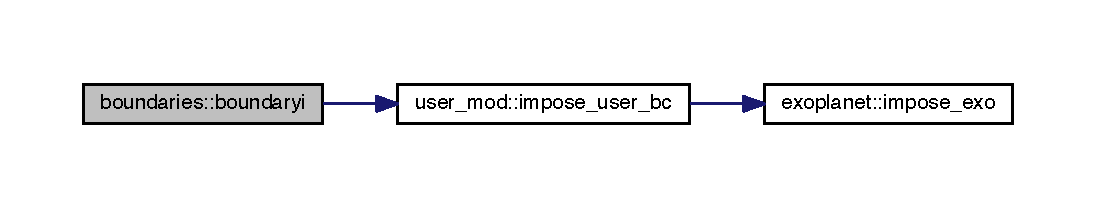
\includegraphics[width=350pt]{namespaceboundaries_a3742debeb694e374aed0d5b1e6970b8a_cgraph}
\end{center}
\end{figure}


\hypertarget{namespaceboundaries_ae74a7f6b33366d1adac94ac3bc438104}{}\index{boundaries@{boundaries}!boundaryii@{boundaryii}}
\index{boundaryii@{boundaryii}!boundaries@{boundaries}}
\subsubsection[{boundaryii}]{\setlength{\rightskip}{0pt plus 5cm}subroutine boundaries\+::boundaryii (
\begin{DoxyParamCaption}
\item[{real, intent(in), optional}]{time, }
\item[{real, intent(in), optional}]{dt}
\end{DoxyParamCaption}
)}\label{namespaceboundaries_ae74a7f6b33366d1adac94ac3bc438104}
Boundary conditions for 2nd order half timestep ~\newline
 The conditions only are imposed in two ghost cells on the up (stepped) variables 
\begin{DoxyParams}{Parameters}
{\em real} & \mbox{[}in\mbox{]} optional, time \+: integration time \\
\hline
{\em real} & \mbox{[}in\mbox{]} optional, dt \+: timestep \\
\hline
\end{DoxyParams}


Definition at line 264 of file boundaries.\+f90.



Here is the call graph for this function\+:\nopagebreak
\begin{figure}[H]
\begin{center}
\leavevmode
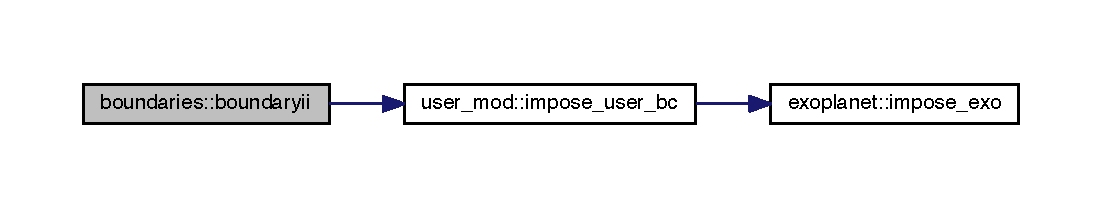
\includegraphics[width=350pt]{namespaceboundaries_ae74a7f6b33366d1adac94ac3bc438104_cgraph}
\end{center}
\end{figure}



\hypertarget{namespacechemistry}{}\section{chemistry Module Reference}
\label{namespacechemistry}\index{chemistry@{chemistry}}


chenistry module  


\subsection*{Functions/\+Subroutines}
\begin{DoxyCompactItemize}
\item 
subroutine \hyperlink{namespacechemistry_a33dc05889bfc2d0361a4a3f95086f68c}{update\+\_\+chem} ()
\begin{DoxyCompactList}\small\item\em Advances the chemistry network. \end{DoxyCompactList}\item 
subroutine \hyperlink{namespacechemistry_ab808252fa02b3bfb1ac29ed7b2f5122e}{chemstep} (y, y0, T, deltt)
\begin{DoxyCompactList}\small\item\em Advances the chemistry network in one cell. \end{DoxyCompactList}\end{DoxyCompactItemize}


\subsection{Detailed Description}
module to solve the chemical/ionic network, and estimate the cooling assiciated with it. 

\subsection{Function/\+Subroutine Documentation}
\hypertarget{namespacechemistry_ab808252fa02b3bfb1ac29ed7b2f5122e}{}\index{chemistry@{chemistry}!chemstep@{chemstep}}
\index{chemstep@{chemstep}!chemistry@{chemistry}}
\subsubsection[{chemstep}]{\setlength{\rightskip}{0pt plus 5cm}subroutine chemistry\+::chemstep (
\begin{DoxyParamCaption}
\item[{real (kind=8), dimension(n\+\_\+spec), intent(inout)}]{y, }
\item[{real (kind=8), dimension(n\+\_\+elem), intent(in)}]{y0, }
\item[{real (kind=8), intent(in)}]{T, }
\item[{real (kind=8), intent(in)}]{deltt}
\end{DoxyParamCaption}
)}\label{namespacechemistry_ab808252fa02b3bfb1ac29ed7b2f5122e}
Advances the chemistry network on the in one cell 
\begin{DoxyParams}{Parameters}
{\em real} & \mbox{[}inout\mbox{]} y(n\+\_\+spec) \+: number densities of the species to be updated by the chemistry \\
\hline
{\em real} & \mbox{[}in\mbox{]} y\mbox{[}n\+\_\+elem\mbox{]} \+: total number density of each of the elements involved in the reactions \\
\hline
{\em real} & \mbox{[}in\mbox{]} T \+: Temperature \mbox{[}K\mbox{]} \\
\hline
{\em real} & \mbox{[}in\mbox{]} deltt \+: time interval (from the hydro, in seconds) \\
\hline
\end{DoxyParams}


Definition at line 92 of file chemistry.\+f90.



Here is the call graph for this function\+:
% FIG 0


\hypertarget{namespacechemistry_a33dc05889bfc2d0361a4a3f95086f68c}{}\index{chemistry@{chemistry}!update\+\_\+chem@{update\+\_\+chem}}
\index{update\+\_\+chem@{update\+\_\+chem}!chemistry@{chemistry}}
\subsubsection[{update\+\_\+chem}]{\setlength{\rightskip}{0pt plus 5cm}subroutine chemistry\+::update\+\_\+chem (
\begin{DoxyParamCaption}
{}
\end{DoxyParamCaption}
)}\label{namespacechemistry_a33dc05889bfc2d0361a4a3f95086f68c}
Advances the chemistry network on the entire domain (except ghost cells), updates primitives and conserved variables in globals 

Definition at line 44 of file chemistry.\+f90.



Here is the call graph for this function\+:
% FIG 1



\hypertarget{namespacecoldens__utilities}{}\section{coldens\+\_\+utilities Module Reference}
\label{namespacecoldens__utilities}\index{coldens\+\_\+utilities@{coldens\+\_\+utilities}}


Column densirt projection.  


\subsection*{Functions/\+Subroutines}
\begin{DoxyCompactItemize}
\item 
subroutine \hyperlink{namespacecoldens__utilities_a9fa20a511c2b17a33fdb8fc1b3bf55a2}{init\+\_\+coldens} ()
\begin{DoxyCompactList}\small\item\em Initializes data. \end{DoxyCompactList}\item 
subroutine \hyperlink{namespacecoldens__utilities_a2dafe54f1edb888f313949f4f801e2d6}{read\+\_\+data} (u, itprint, filepath)
\begin{DoxyCompactList}\small\item\em reads data from file \end{DoxyCompactList}\item 
subroutine \hyperlink{namespacecoldens__utilities_a7df7ce1cf8187ca5393dc35effa22020}{getxyz} (i, j, k, x, y, z)
\begin{DoxyCompactList}\small\item\em gets position of a cell \end{DoxyCompactList}\item 
subroutine \hyperlink{namespacecoldens__utilities_af7f94bfb5ffee491708d3f221915abcf}{rotation\+\_\+x} (theta, x, y, z, xn, yn, zn)
\begin{DoxyCompactList}\small\item\em Rotation around the X axis. \end{DoxyCompactList}\item 
subroutine \hyperlink{namespacecoldens__utilities_a989fb82adc69b6b1c00a2d2400c9854a}{rotation\+\_\+y} (theta, x, y, z, xn, yn, zn)
\begin{DoxyCompactList}\small\item\em Rotation around the Y axis. \end{DoxyCompactList}\item 
subroutine \hyperlink{namespacecoldens__utilities_a062761acebb4d5a76b3706256a491687}{rotation\+\_\+z} (theta, x, y, z, xn, yn, zn)
\begin{DoxyCompactList}\small\item\em Rotation around the Z axis. \end{DoxyCompactList}\item 
subroutine \hyperlink{namespacecoldens__utilities_af035b829538114f8b62f54365269bdab}{fill\+\_\+map} (nxmap, nymap, u, map, dx\+T, dy\+T, theta\+\_\+x, theta\+\_\+y, theta\+\_\+z)
\begin{DoxyCompactList}\small\item\em Fill target map. \end{DoxyCompactList}\item 
subroutine \hyperlink{namespacecoldens__utilities_a78891c0c5736f8d50bf07d19757e7237}{write\+\_\+map} (fileout, nxmap, nymap, map)
\begin{DoxyCompactList}\small\item\em Writes projection to file. \end{DoxyCompactList}\end{DoxyCompactItemize}


\subsection{Detailed Description}
Utilities to compute a column density map 

\subsection{Function/\+Subroutine Documentation}
\hypertarget{namespacecoldens__utilities_af035b829538114f8b62f54365269bdab}{}\index{coldens\+\_\+utilities@{coldens\+\_\+utilities}!fill\+\_\+map@{fill\+\_\+map}}
\index{fill\+\_\+map@{fill\+\_\+map}!coldens\+\_\+utilities@{coldens\+\_\+utilities}}
\subsubsection[{fill\+\_\+map}]{\setlength{\rightskip}{0pt plus 5cm}subroutine coldens\+\_\+utilities\+::fill\+\_\+map (
\begin{DoxyParamCaption}
\item[{integer, intent(in)}]{nxmap, }
\item[{integer, intent(in)}]{nymap, }
\item[{real, dimension(neq,nxmin\+:nxmax,nymin\+:nymax, nzmin\+:nzmax), intent(in)}]{u, }
\item[{real, dimension(nxmap,nymap), intent(out)}]{map, }
\item[{real, intent(in)}]{dx\+T, }
\item[{real, intent(in)}]{dy\+T, }
\item[{real, intent(in)}]{theta\+\_\+x, }
\item[{real, intent(in)}]{theta\+\_\+y, }
\item[{real, intent(in)}]{theta\+\_\+z}
\end{DoxyParamCaption}
)}\label{namespacecoldens__utilities_af035b829538114f8b62f54365269bdab}
Fills the target map of one M\+P\+I block 
\begin{DoxyParams}{Parameters}
{\em integer} & \mbox{[}in\mbox{]} nxmap \+: Number of X cells in target \\
\hline
{\em integer} & \mbox{[}in\mbox{]} nymap \+: Number of Y cells in target \\
\hline
{\em real} & \mbox{[}in\mbox{]} u(neq,nxmin\+:nxmax,nymin\+:nymax, nzmin\+:nzmax) \+: conserved variables \\
\hline
{\em real} & \mbox{[}out\mbox{]} map(nxmap,mymap) \+: Target map \\
\hline
{\em real} & \mbox{[}in\mbox{]} dx\+T \+: target pixel width \\
\hline
{\em real} & \mbox{[}in\mbox{]} dy\+T \+: target pixel height \\
\hline
{\em real} & \mbox{[}in\mbox{]} thetax \+: Rotation around X \\
\hline
{\em real} & \mbox{[}in\mbox{]} thetay \+: Rotation around Y \\
\hline
{\em real} & \mbox{[}in\mbox{]} thetaz \+: Rotation around Z \\
\hline
\end{DoxyParams}


Definition at line 286 of file coldens.\+f90.



Here is the call graph for this function\+:\nopagebreak
\begin{figure}[H]
\begin{center}
\leavevmode
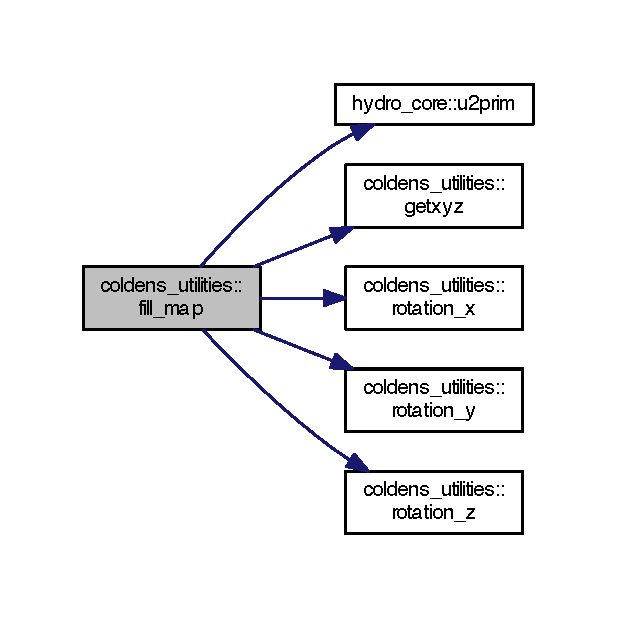
\includegraphics[width=296pt]{namespacecoldens__utilities_af035b829538114f8b62f54365269bdab_cgraph}
\end{center}
\end{figure}


\hypertarget{namespacecoldens__utilities_a7df7ce1cf8187ca5393dc35effa22020}{}\index{coldens\+\_\+utilities@{coldens\+\_\+utilities}!getxyz@{getxyz}}
\index{getxyz@{getxyz}!coldens\+\_\+utilities@{coldens\+\_\+utilities}}
\subsubsection[{getxyz}]{\setlength{\rightskip}{0pt plus 5cm}subroutine coldens\+\_\+utilities\+::getxyz (
\begin{DoxyParamCaption}
\item[{integer, intent(in)}]{i, }
\item[{integer, intent(in)}]{j, }
\item[{integer, intent(in)}]{k, }
\item[{real, intent(out)}]{x, }
\item[{real, intent(out)}]{y, }
\item[{real, intent(out)}]{z}
\end{DoxyParamCaption}
)}\label{namespacecoldens__utilities_a7df7ce1cf8187ca5393dc35effa22020}
Returns the position and spherical radius calculated with respect to the center of the grid 
\begin{DoxyParams}{Parameters}
{\em integer} & \mbox{[}in\mbox{]} i \+: cell index in the x direction \\
\hline
{\em integer} & \mbox{[}in\mbox{]} j \+: cell index in the y direction \\
\hline
{\em integer} & \mbox{[}in\mbox{]} k \+: cell index in the z direction \\
\hline
{\em real} & \mbox{[}in\mbox{]} x \+: x position in the grid \\
\hline
{\em real} & \mbox{[}in\mbox{]} y \+: y position in the grid \\
\hline
{\em real} & \mbox{[}in\mbox{]} z \+: z position in the grid \\
\hline
\end{DoxyParams}


Definition at line 188 of file coldens.\+f90.

\hypertarget{namespacecoldens__utilities_a9fa20a511c2b17a33fdb8fc1b3bf55a2}{}\index{coldens\+\_\+utilities@{coldens\+\_\+utilities}!init\+\_\+coldens@{init\+\_\+coldens}}
\index{init\+\_\+coldens@{init\+\_\+coldens}!coldens\+\_\+utilities@{coldens\+\_\+utilities}}
\subsubsection[{init\+\_\+coldens}]{\setlength{\rightskip}{0pt plus 5cm}subroutine coldens\+\_\+utilities\+::init\+\_\+coldens (
\begin{DoxyParamCaption}
{}
\end{DoxyParamCaption}
)}\label{namespacecoldens__utilities_a9fa20a511c2b17a33fdb8fc1b3bf55a2}
Initializes data, M\+P\+I and other stuff 

Definition at line 36 of file coldens.\+f90.

\hypertarget{namespacecoldens__utilities_a2dafe54f1edb888f313949f4f801e2d6}{}\index{coldens\+\_\+utilities@{coldens\+\_\+utilities}!read\+\_\+data@{read\+\_\+data}}
\index{read\+\_\+data@{read\+\_\+data}!coldens\+\_\+utilities@{coldens\+\_\+utilities}}
\subsubsection[{read\+\_\+data}]{\setlength{\rightskip}{0pt plus 5cm}subroutine coldens\+\_\+utilities\+::read\+\_\+data (
\begin{DoxyParamCaption}
\item[{real, dimension(neq,nxmin\+:nxmax,nymin\+:nymax,nzmin\+:nzmax), intent(out)}]{u, }
\item[{integer, intent(in)}]{itprint, }
\item[{character (len=128), intent(in)}]{filepath}
\end{DoxyParamCaption}
)}\label{namespacecoldens__utilities_a2dafe54f1edb888f313949f4f801e2d6}
reads data from file 
\begin{DoxyParams}{Parameters}
{\em real} & \mbox{[}out\mbox{]} u(neq,nxmin\+:nxmax,nymin\+:nymax,nzmin\+:nzmax) \+: conserved variables \\
\hline
{\em integer} & \mbox{[}in\mbox{]} itprint \+: number of output \\
\hline
{\em string} & \mbox{[}in\mbox{]} filepath \+: path where the output is \\
\hline
\end{DoxyParams}


Definition at line 135 of file coldens.\+f90.

\hypertarget{namespacecoldens__utilities_af7f94bfb5ffee491708d3f221915abcf}{}\index{coldens\+\_\+utilities@{coldens\+\_\+utilities}!rotation\+\_\+x@{rotation\+\_\+x}}
\index{rotation\+\_\+x@{rotation\+\_\+x}!coldens\+\_\+utilities@{coldens\+\_\+utilities}}
\subsubsection[{rotation\+\_\+x}]{\setlength{\rightskip}{0pt plus 5cm}subroutine coldens\+\_\+utilities\+::rotation\+\_\+x (
\begin{DoxyParamCaption}
\item[{real, intent(in)}]{theta, }
\item[{real, intent(in)}]{x, }
\item[{real, intent(in)}]{y, }
\item[{real, intent(in)}]{z, }
\item[{real, intent(out)}]{xn, }
\item[{real, intent(out)}]{yn, }
\item[{real, intent(out)}]{zn}
\end{DoxyParamCaption}
)}\label{namespacecoldens__utilities_af7f94bfb5ffee491708d3f221915abcf}
Does a rotation around the x axis 
\begin{DoxyParams}{Parameters}
{\em real} & \mbox{[}in\mbox{]}, theta \+: Angle of rotation (in radians) \\
\hline
{\em real} & \mbox{[}in\mbox{]}, x \+: original x position in the grid \\
\hline
{\em real} & \mbox{[}in\mbox{]}, y \+: original y position in the grid \\
\hline
{\em real} & \mbox{[}in\mbox{]}, x \+: original z position in the grid \\
\hline
{\em real} & \mbox{[}out\mbox{]}, x \+: final x position in the grid \\
\hline
{\em real} & \mbox{[}out\mbox{]}, y \+: final y position in the grid \\
\hline
{\em real} & \mbox{[}out\mbox{]}, x \+: final z position in the grid \\
\hline
\end{DoxyParams}


Definition at line 214 of file coldens.\+f90.

\hypertarget{namespacecoldens__utilities_a989fb82adc69b6b1c00a2d2400c9854a}{}\index{coldens\+\_\+utilities@{coldens\+\_\+utilities}!rotation\+\_\+y@{rotation\+\_\+y}}
\index{rotation\+\_\+y@{rotation\+\_\+y}!coldens\+\_\+utilities@{coldens\+\_\+utilities}}
\subsubsection[{rotation\+\_\+y}]{\setlength{\rightskip}{0pt plus 5cm}subroutine coldens\+\_\+utilities\+::rotation\+\_\+y (
\begin{DoxyParamCaption}
\item[{real, intent(in)}]{theta, }
\item[{real, intent(in)}]{x, }
\item[{real, intent(in)}]{y, }
\item[{real, intent(in)}]{z, }
\item[{real, intent(out)}]{xn, }
\item[{real, intent(out)}]{yn, }
\item[{real, intent(out)}]{zn}
\end{DoxyParamCaption}
)}\label{namespacecoldens__utilities_a989fb82adc69b6b1c00a2d2400c9854a}
Does a rotation around the x axis 
\begin{DoxyParams}{Parameters}
{\em real} & \mbox{[}in\mbox{]}, theta \+: Angle of rotation (in radians) \\
\hline
{\em real} & \mbox{[}in\mbox{]}, x \+: original x position in the grid \\
\hline
{\em real} & \mbox{[}in\mbox{]}, y \+: original y position in the grid \\
\hline
{\em real} & \mbox{[}in\mbox{]}, x \+: original z position in the grid \\
\hline
{\em real} & \mbox{[}out\mbox{]}, x \+: final x position in the grid \\
\hline
{\em real} & \mbox{[}out\mbox{]}, y \+: final y position in the grid \\
\hline
{\em real} & \mbox{[}out\mbox{]}, x \+: final z position in the grid \\
\hline
\end{DoxyParams}


Definition at line 238 of file coldens.\+f90.

\hypertarget{namespacecoldens__utilities_a062761acebb4d5a76b3706256a491687}{}\index{coldens\+\_\+utilities@{coldens\+\_\+utilities}!rotation\+\_\+z@{rotation\+\_\+z}}
\index{rotation\+\_\+z@{rotation\+\_\+z}!coldens\+\_\+utilities@{coldens\+\_\+utilities}}
\subsubsection[{rotation\+\_\+z}]{\setlength{\rightskip}{0pt plus 5cm}subroutine coldens\+\_\+utilities\+::rotation\+\_\+z (
\begin{DoxyParamCaption}
\item[{real, intent(in)}]{theta, }
\item[{real, intent(in)}]{x, }
\item[{real, intent(in)}]{y, }
\item[{real, intent(in)}]{z, }
\item[{real, intent(out)}]{xn, }
\item[{real, intent(out)}]{yn, }
\item[{real, intent(out)}]{zn}
\end{DoxyParamCaption}
)}\label{namespacecoldens__utilities_a062761acebb4d5a76b3706256a491687}
Does a rotation around the x axis 
\begin{DoxyParams}{Parameters}
{\em real} & \mbox{[}in\mbox{]}, theta \+: Angle of rotation (in radians) \\
\hline
{\em real} & \mbox{[}in\mbox{]}, x \+: original x position in the grid \\
\hline
{\em real} & \mbox{[}in\mbox{]}, y \+: original y position in the grid \\
\hline
{\em real} & \mbox{[}in\mbox{]}, x \+: original z position in the grid \\
\hline
{\em real} & \mbox{[}out\mbox{]}, x \+: final x position in the grid \\
\hline
{\em real} & \mbox{[}out\mbox{]}, y \+: final y position in the grid \\
\hline
{\em real} & \mbox{[}out\mbox{]}, x \+: final z position in the grid \\
\hline
\end{DoxyParams}


Definition at line 260 of file coldens.\+f90.

\hypertarget{namespacecoldens__utilities_a78891c0c5736f8d50bf07d19757e7237}{}\index{coldens\+\_\+utilities@{coldens\+\_\+utilities}!write\+\_\+map@{write\+\_\+map}}
\index{write\+\_\+map@{write\+\_\+map}!coldens\+\_\+utilities@{coldens\+\_\+utilities}}
\subsubsection[{write\+\_\+map}]{\setlength{\rightskip}{0pt plus 5cm}subroutine coldens\+\_\+utilities\+::write\+\_\+map (
\begin{DoxyParamCaption}
\item[{character (len=128), intent(in)}]{fileout, }
\item[{integer, intent(in)}]{nxmap, }
\item[{integer, intent(in)}]{nymap, }
\item[{real, dimension(nxmap,nymap), intent(in)}]{map}
\end{DoxyParamCaption}
)}\label{namespacecoldens__utilities_a78891c0c5736f8d50bf07d19757e7237}
Writes projection to file 
\begin{DoxyParams}{Parameters}
{\em integer} & \mbox{[}in\mbox{]} itprint \+: number of output \\
\hline
{\em string} & \mbox{[}in\mbox{]} fileout \+: file where to write \\
\hline
{\em integer} & \mbox{[}in\mbox{]} nxmap \+: Number of X cells in target \\
\hline
{\em integer} & \mbox{[}in\mbox{]} nymap \+: Number of Y cells in target \\
\hline
{\em real} & \mbox{[}in\mbox{]} map(nxmap,mymap) \+: Target map \\
\hline
\end{DoxyParams}


Definition at line 340 of file coldens.\+f90.


\hypertarget{namespaceconstants}{}\section{constants Module Reference}
\label{namespaceconstants}\index{constants@{constants}}


Module containing physical and asronomical constants.  


\subsection*{Variables}
\begin{DoxyCompactItemize}
\item 
\hypertarget{namespaceconstants_a815ad954ef712211ed1b1fdb8be42487}{}real, parameter \hyperlink{namespaceconstants_a815ad954ef712211ed1b1fdb8be42487}{pi} =acos(-\/1.)\label{namespaceconstants_a815ad954ef712211ed1b1fdb8be42487}

\begin{DoxyCompactList}\small\item\em $ \pi $ \end{DoxyCompactList}\item 
\hypertarget{namespaceconstants_aac258d92ad409a5ad7f8748101e932b0}{}real, parameter \hyperlink{namespaceconstants_aac258d92ad409a5ad7f8748101e932b0}{amh} =1.\+66e-\/24\label{namespaceconstants_aac258d92ad409a5ad7f8748101e932b0}

\begin{DoxyCompactList}\small\item\em hydrogen mass \end{DoxyCompactList}\item 
\hypertarget{namespaceconstants_afc7b29a52df069e705256c11de562808}{}real, parameter \hyperlink{namespaceconstants_afc7b29a52df069e705256c11de562808}{kb} =1.\+38e-\/16\label{namespaceconstants_afc7b29a52df069e705256c11de562808}

\begin{DoxyCompactList}\small\item\em Boltzmann constant (cgs) \end{DoxyCompactList}\item 
\hypertarget{namespaceconstants_aab4c0a2b0e8b8cda79e9d683b3e650f6}{}real, parameter \hyperlink{namespaceconstants_aab4c0a2b0e8b8cda79e9d683b3e650f6}{rg} =8.\+3145e7\label{namespaceconstants_aab4c0a2b0e8b8cda79e9d683b3e650f6}

\begin{DoxyCompactList}\small\item\em Gas constant (cgs) \end{DoxyCompactList}\item 
\hypertarget{namespaceconstants_a1e2651b5b314d8b869a9a48b1063f126}{}real, parameter \hyperlink{namespaceconstants_a1e2651b5b314d8b869a9a48b1063f126}{ggrav} =6.\+67259e-\/8\label{namespaceconstants_a1e2651b5b314d8b869a9a48b1063f126}

\begin{DoxyCompactList}\small\item\em Gravitational constant (cgs) \end{DoxyCompactList}\item 
\hypertarget{namespaceconstants_ac15de49d1114e2e8d78a3e77e2c0ebd0}{}real, parameter \hyperlink{namespaceconstants_ac15de49d1114e2e8d78a3e77e2c0ebd0}{clight} =2.\+99\+E10\label{namespaceconstants_ac15de49d1114e2e8d78a3e77e2c0ebd0}

\begin{DoxyCompactList}\small\item\em speed of light in vacuum (cgs) \end{DoxyCompactList}\item 
\hypertarget{namespaceconstants_a47dcdcdf147127ab93252565436ce046}{}real, parameter \hyperlink{namespaceconstants_a47dcdcdf147127ab93252565436ce046}{msun} =1.\+99\+E33\label{namespaceconstants_a47dcdcdf147127ab93252565436ce046}

\begin{DoxyCompactList}\small\item\em solar radius (cgs) \end{DoxyCompactList}\item 
\hypertarget{namespaceconstants_a86e80095a8a44315466905ab42ec2814}{}real, parameter \hyperlink{namespaceconstants_a86e80095a8a44315466905ab42ec2814}{rsun} =6.\+955e10\label{namespaceconstants_a86e80095a8a44315466905ab42ec2814}

\begin{DoxyCompactList}\small\item\em solar mass (cgs) \end{DoxyCompactList}\item 
\hypertarget{namespaceconstants_a399e5e2bceae23d80dfe33489603dfa5}{}real, parameter \hyperlink{namespaceconstants_a399e5e2bceae23d80dfe33489603dfa5}{mjup} =1.\+898\+E30\label{namespaceconstants_a399e5e2bceae23d80dfe33489603dfa5}

\begin{DoxyCompactList}\small\item\em Jupiter mass (cgs) \end{DoxyCompactList}\item 
\hypertarget{namespaceconstants_a4cbd85fb12d8faa8be8463982fa6fd29}{}real, parameter \hyperlink{namespaceconstants_a4cbd85fb12d8faa8be8463982fa6fd29}{rjup} =7.\+1492\+E9\label{namespaceconstants_a4cbd85fb12d8faa8be8463982fa6fd29}

\begin{DoxyCompactList}\small\item\em Jupiter radius (cgs) \end{DoxyCompactList}\item 
\hypertarget{namespaceconstants_aba9a695c84a59f13c2d528a170a43b65}{}real, parameter \hyperlink{namespaceconstants_aba9a695c84a59f13c2d528a170a43b65}{au} =1.\+496e13\label{namespaceconstants_aba9a695c84a59f13c2d528a170a43b65}

\begin{DoxyCompactList}\small\item\em 1\+A\+U in cm \end{DoxyCompactList}\item 
\hypertarget{namespaceconstants_aa5d9aea15e53a1abbc29e5f419b38601}{}real, parameter \hyperlink{namespaceconstants_aa5d9aea15e53a1abbc29e5f419b38601}{pc} =3.\+0857\+E18\label{namespaceconstants_aa5d9aea15e53a1abbc29e5f419b38601}

\begin{DoxyCompactList}\small\item\em 1pc in cm \end{DoxyCompactList}\item 
\hypertarget{namespaceconstants_aee24dfdb51a8ed33a59bb80e98938718}{}real, parameter \hyperlink{namespaceconstants_aee24dfdb51a8ed33a59bb80e98938718}{kpc} =3.\+0857\+E21\label{namespaceconstants_aee24dfdb51a8ed33a59bb80e98938718}

\begin{DoxyCompactList}\small\item\em 1\+Kpc in cm \end{DoxyCompactList}\item 
\hypertarget{namespaceconstants_a1c0cbdbdc4f321db2055f6cd61cdd3f4}{}real, parameter \hyperlink{namespaceconstants_a1c0cbdbdc4f321db2055f6cd61cdd3f4}{hr} =3600.\label{namespaceconstants_a1c0cbdbdc4f321db2055f6cd61cdd3f4}

\begin{DoxyCompactList}\small\item\em 1hr in seconds \end{DoxyCompactList}\item 
\hypertarget{namespaceconstants_a9578082af66e4af5e4101e39b4abde29}{}real, parameter \hyperlink{namespaceconstants_a9578082af66e4af5e4101e39b4abde29}{day} =86400.\label{namespaceconstants_a9578082af66e4af5e4101e39b4abde29}

\begin{DoxyCompactList}\small\item\em 1day in seconds \end{DoxyCompactList}\item 
\hypertarget{namespaceconstants_a1fd58880de7afc0479eb60d136bac8b2}{}real, parameter \hyperlink{namespaceconstants_a1fd58880de7afc0479eb60d136bac8b2}{yr} =3.\+1536\+E7\label{namespaceconstants_a1fd58880de7afc0479eb60d136bac8b2}

\begin{DoxyCompactList}\small\item\em 1yr in seconds \end{DoxyCompactList}\item 
\hypertarget{namespaceconstants_af554c9cfbc1f3c74a8176265ea5370dd}{}real, parameter \hyperlink{namespaceconstants_af554c9cfbc1f3c74a8176265ea5370dd}{myr} =3.\+1536\+E13\label{namespaceconstants_af554c9cfbc1f3c74a8176265ea5370dd}

\begin{DoxyCompactList}\small\item\em 1\+Myr in seconds \end{DoxyCompactList}\end{DoxyCompactItemize}

\hypertarget{namespacecooling__chi}{}\section{cooling\+\_\+chi Module Reference}
\label{namespacecooling__chi}\index{cooling\+\_\+chi@{cooling\+\_\+chi}}


Cooling module with C\+H\+I\+A\+N\+T\+I generated cooling curves.  


\subsection*{Functions/\+Subroutines}
\begin{DoxyCompactItemize}
\item 
subroutine \hyperlink{namespacecooling__chi_acdcfaea636dd68b666577d8daf434d35}{read\+\_\+table} ()
\begin{DoxyCompactList}\small\item\em Reads the cooling curve table. \end{DoxyCompactList}\item 
real(kind=8) function \hyperlink{namespacecooling__chi_a20c87eb43e4f324fa7d83fe9174fd767}{coolchi} (T)
\begin{DoxyCompactList}\small\item\em Returns the cooling coefficient interpolating the table. \end{DoxyCompactList}\item 
subroutine \hyperlink{namespacecooling__chi_a666df501be07ce1e3612d3c3796cf2a3}{coolingchi} ()
\begin{DoxyCompactList}\small\item\em High level wrapper to apply cooling with C\+H\+I\+A\+N\+T\+I tables. \end{DoxyCompactList}\end{DoxyCompactItemize}
\subsection*{Variables}
\begin{DoxyCompactItemize}
\item 
\hypertarget{namespacecooling__chi_a37baf8c1757edb98fcaa8b62587d7b2f}{}real(kind=8), dimension(2, 41) {\bfseries cooltab}\label{namespacecooling__chi_a37baf8c1757edb98fcaa8b62587d7b2f}

\end{DoxyCompactItemize}


\subsection{Detailed Description}
Cooling module with C\+H\+I\+A\+N\+T\+I generated cooling curves ~\newline
 The location of the tables is assumed to be in src/\+C\+H\+I\+A\+N\+T\+Ilib/cooling\+C\+H\+I\+A\+N\+T\+I.\+tab 

\subsection{Function/\+Subroutine Documentation}
\hypertarget{namespacecooling__chi_a20c87eb43e4f324fa7d83fe9174fd767}{}\index{cooling\+\_\+chi@{cooling\+\_\+chi}!coolchi@{coolchi}}
\index{coolchi@{coolchi}!cooling\+\_\+chi@{cooling\+\_\+chi}}
\subsubsection[{coolchi}]{\setlength{\rightskip}{0pt plus 5cm}real (kind=8) function cooling\+\_\+chi\+::coolchi (
\begin{DoxyParamCaption}
\item[{real, intent(in)}]{T}
\end{DoxyParamCaption}
)}\label{namespacecooling__chi_a20c87eb43e4f324fa7d83fe9174fd767}

\begin{DoxyParams}{Parameters}
{\em real} & \mbox{[}in\mbox{]} T \+: Temperature K \\
\hline
\end{DoxyParams}


Definition at line 75 of file cooling\+\_\+chi.\+f90.

\hypertarget{namespacecooling__chi_a666df501be07ce1e3612d3c3796cf2a3}{}\index{cooling\+\_\+chi@{cooling\+\_\+chi}!coolingchi@{coolingchi}}
\index{coolingchi@{coolingchi}!cooling\+\_\+chi@{cooling\+\_\+chi}}
\subsubsection[{coolingchi}]{\setlength{\rightskip}{0pt plus 5cm}subroutine cooling\+\_\+chi\+::coolingchi (
\begin{DoxyParamCaption}
{}
\end{DoxyParamCaption}
)}\label{namespacecooling__chi_a666df501be07ce1e3612d3c3796cf2a3}
High level wrapper to apply cooling with C\+H\+I\+A\+N\+T\+I tables ~\newline
 cooling is applied in the entire domain and updates both the conserved and primitive variables 

Definition at line 102 of file cooling\+\_\+chi.\+f90.



Here is the call graph for this function\+:
% FIG 0


\hypertarget{namespacecooling__chi_acdcfaea636dd68b666577d8daf434d35}{}\index{cooling\+\_\+chi@{cooling\+\_\+chi}!read\+\_\+table@{read\+\_\+table}}
\index{read\+\_\+table@{read\+\_\+table}!cooling\+\_\+chi@{cooling\+\_\+chi}}
\subsubsection[{read\+\_\+table}]{\setlength{\rightskip}{0pt plus 5cm}subroutine cooling\+\_\+chi\+::read\+\_\+table (
\begin{DoxyParamCaption}
{}
\end{DoxyParamCaption}
)}\label{namespacecooling__chi_acdcfaea636dd68b666577d8daf434d35}
Reads the cooling curve table generated by C\+H\+U\+A\+N\+T\+I, the location is assumed in /src/\+C\+H\+I\+A\+N\+T\+Ilib/cooling\+C\+H\+I\+A\+N\+T\+I.tab 

Definition at line 44 of file cooling\+\_\+chi.\+f90.


\hypertarget{namespacecooling__dmc}{}\section{cooling\+\_\+dmc Module Reference}
\label{namespacecooling__dmc}\index{cooling\+\_\+dmc@{cooling\+\_\+dmc}}


Cooling module with Dalgarno Mc\+Cray coronal cooling curve.  


\subsection*{Functions/\+Subroutines}
\begin{DoxyCompactItemize}
\item 
subroutine \hyperlink{namespacecooling__dmc_a7874b4f8a76399e87e0a22aecd088cf8}{read\+\_\+table} ()
\begin{DoxyCompactList}\small\item\em Reads the cooling curve table. \end{DoxyCompactList}\item 
real(kind=8) function \hyperlink{namespacecooling__dmc_af987bbf144f596d57b154427bbb82ae5}{cooldmc} (T)
\begin{DoxyCompactList}\small\item\em Returns the cooling coefficient interpolating the table. \end{DoxyCompactList}\item 
subroutine \hyperlink{namespacecooling__dmc_a7af28062f0cd20c4bb0d86c895f4a8d6}{coolingdmc} ()
\begin{DoxyCompactList}\small\item\em High level wrapper to apply cooling with D\+M\+C table. \end{DoxyCompactList}\end{DoxyCompactItemize}
\subsection*{Variables}
\begin{DoxyCompactItemize}
\item 
\hypertarget{namespacecooling__dmc_aa692bc7125c6e889f3cf993f9f48f9d3}{}real(kind=8), dimension(2, 41) {\bfseries cooltab}\label{namespacecooling__dmc_aa692bc7125c6e889f3cf993f9f48f9d3}

\end{DoxyCompactItemize}


\subsection{Detailed Description}
Cooling module with Dalgarno Mc\+Cray coronal cooling curve ~\newline
 The location of the tables is assumed to be in src/\+D\+M\+Clib/cooling\+D\+M\+C.\+tab, it is read by init subroutine 

\subsection{Function/\+Subroutine Documentation}
\hypertarget{namespacecooling__dmc_af987bbf144f596d57b154427bbb82ae5}{}\index{cooling\+\_\+dmc@{cooling\+\_\+dmc}!cooldmc@{cooldmc}}
\index{cooldmc@{cooldmc}!cooling\+\_\+dmc@{cooling\+\_\+dmc}}
\subsubsection[{cooldmc}]{\setlength{\rightskip}{0pt plus 5cm}real (kind=8) function cooling\+\_\+dmc\+::cooldmc (
\begin{DoxyParamCaption}
\item[{real, intent(in)}]{T}
\end{DoxyParamCaption}
)}\label{namespacecooling__dmc_af987bbf144f596d57b154427bbb82ae5}

\begin{DoxyParams}{Parameters}
{\em real} & \mbox{[}in\mbox{]} T \+: Temperature K \\
\hline
\end{DoxyParams}


Definition at line 77 of file cooling\+\_\+dmc.\+f90.

\hypertarget{namespacecooling__dmc_a7af28062f0cd20c4bb0d86c895f4a8d6}{}\index{cooling\+\_\+dmc@{cooling\+\_\+dmc}!coolingdmc@{coolingdmc}}
\index{coolingdmc@{coolingdmc}!cooling\+\_\+dmc@{cooling\+\_\+dmc}}
\subsubsection[{coolingdmc}]{\setlength{\rightskip}{0pt plus 5cm}subroutine cooling\+\_\+dmc\+::coolingdmc (
\begin{DoxyParamCaption}
{}
\end{DoxyParamCaption}
)}\label{namespacecooling__dmc_a7af28062f0cd20c4bb0d86c895f4a8d6}
High level wrapper to apply cooling with D\+M\+C table ~\newline
 cooling is applied in the entire domain and updates both the conserved and primitive variables 

Definition at line 103 of file cooling\+\_\+dmc.\+f90.



Here is the call graph for this function\+:
% FIG 0


\hypertarget{namespacecooling__dmc_a7874b4f8a76399e87e0a22aecd088cf8}{}\index{cooling\+\_\+dmc@{cooling\+\_\+dmc}!read\+\_\+table@{read\+\_\+table}}
\index{read\+\_\+table@{read\+\_\+table}!cooling\+\_\+dmc@{cooling\+\_\+dmc}}
\subsubsection[{read\+\_\+table}]{\setlength{\rightskip}{0pt plus 5cm}subroutine cooling\+\_\+dmc\+::read\+\_\+table (
\begin{DoxyParamCaption}
{}
\end{DoxyParamCaption}
)}\label{namespacecooling__dmc_a7874b4f8a76399e87e0a22aecd088cf8}
Reads the Dalgarno Mc\+Cray cooling courve the location is assumed in src/\+D\+M\+Clib/cooling\+D\+M\+C.\+tab, it is read by init subroutine 

Definition at line 45 of file cooling\+\_\+dmc.\+f90.


\hypertarget{namespacecooling__h}{}\section{cooling\+\_\+h Module Reference}
\label{namespacecooling__h}\index{cooling\+\_\+h@{cooling\+\_\+h}}


Cooling with parametrized cooling and H rate equation.  


\subsection*{Functions/\+Subroutines}
\begin{DoxyCompactItemize}
\item 
subroutine \hyperlink{namespacecooling__h_aee85faa3b36e05a8efb05c1588f34ef2}{coolingh} ()
\begin{DoxyCompactList}\small\item\em High level wrapper to apply cooling. \end{DoxyCompactList}\item 
real(kind=8) function \hyperlink{namespacecooling__h_a09de30645cebf531a647b5f53ae143b2}{alpha} (T)
\begin{DoxyCompactList}\small\item\em calculates the recombination rate (case B) \end{DoxyCompactList}\item 
real(kind=8) function \hyperlink{namespacecooling__h_a5454f21ef468add797c58753a1e0c773}{alpha1} (T)
\begin{DoxyCompactList}\small\item\em calculates the recombination rate to level 1 \end{DoxyCompactList}\item 
real(kind=8) function \hyperlink{namespacecooling__h_ad5f1352f8925ccb1b352d6e749465a92}{colf} (T)
\begin{DoxyCompactList}\small\item\em calculates the collisional ionization rate \end{DoxyCompactList}\item 
real(kind=8) function \hyperlink{namespacecooling__h_a2a2de25572bd515eae9441391e0ed0f8}{betah} (T)
\begin{DoxyCompactList}\small\item\em beta\+H(\+T) \end{DoxyCompactList}\item 
real(kind=8) function \hyperlink{namespacecooling__h_a92cfd14c9b02e853eb33d22857fabeed}{aloss} (X1, X2, D\+T, D\+E\+N, D\+H0, T\+E0)
\begin{DoxyCompactList}\small\item\em Non equilibrium cooling. \end{DoxyCompactList}\item 
subroutine \hyperlink{namespacecooling__h_aef95dbca5e7aef78d66a225cc217c982}{atomic} (dt, uu, tau, radphi)
\begin{DoxyCompactList}\small\item\em Updates the ionization fraction and applpies cooling. \end{DoxyCompactList}\end{DoxyCompactItemize}


\subsection{Detailed Description}
Cooling with parametrized cooling and H rate equation 

\subsection{Function/\+Subroutine Documentation}
\hypertarget{namespacecooling__h_a92cfd14c9b02e853eb33d22857fabeed}{}\index{cooling\+\_\+h@{cooling\+\_\+h}!aloss@{aloss}}
\index{aloss@{aloss}!cooling\+\_\+h@{cooling\+\_\+h}}
\subsubsection[{aloss}]{\setlength{\rightskip}{0pt plus 5cm}real (kind=8) function cooling\+\_\+h\+::aloss (
\begin{DoxyParamCaption}
\item[{real (kind=8), intent(in)}]{X1, }
\item[{real (kind=8), intent(in)}]{X2, }
\item[{real, intent(in)}]{D\+T, }
\item[{real (kind=8), intent(in)}]{D\+E\+N, }
\item[{real (kind=8), intent(in)}]{D\+H0, }
\item[{real (kind=8), intent(in)}]{T\+E0}
\end{DoxyParamCaption}
)}\label{namespacecooling__h_a92cfd14c9b02e853eb33d22857fabeed}
Non-\/equilibrium energy loss for low temperatures considering the collisional excitation of \mbox{[}O I\mbox{]} and \mbox{[}O I\+I\mbox{]} lines and radiative recombination of H. This cooling rate is multiplied by a factor of 7.\+033 so that it has the same value as the \char`\"{}coronal equilibrium\char`\"{} cooling rate at a temperature of 44770 K (at temperatures higher than this value, the equilibrium cooling rate is used). The collisional ionization of H and excitation of Lyman-\/alpha are computed separately, and added to the cooling rate. 
\begin{DoxyParams}{Parameters}
{\em real8} & \mbox{[}in\mbox{]} x1 \+: initial H ionization fraction \\
\hline
{\em real8} & \mbox{[}in\mbox{]} x2 \+: final H ionization fraction \\
\hline
{\em real} & \mbox{[}in\mbox{]} dt \+: timestep \\
\hline
{\em real8} & \mbox{[}in\mbox{]} den \+: total density of hydrogen \\
\hline
{\em real8} & \mbox{[}in\mbox{]} dh0 \+: density of neutral hydrogen \\
\hline
{\em real8} & \mbox{[}in\mbox{]} Te0 \+: Temperature \\
\hline
\end{DoxyParams}


Definition at line 164 of file cooling\+\_\+h.\+f90.



Here is the call graph for this function\+:\nopagebreak
\begin{figure}[H]
\begin{center}
\leavevmode
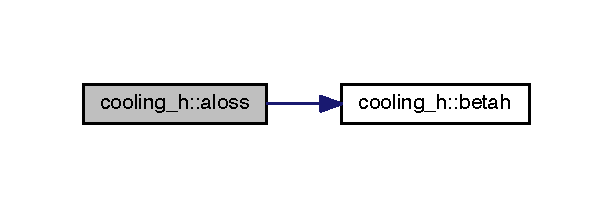
\includegraphics[width=284pt]{namespacecooling__h_a92cfd14c9b02e853eb33d22857fabeed_cgraph}
\end{center}
\end{figure}


\hypertarget{namespacecooling__h_a09de30645cebf531a647b5f53ae143b2}{}\index{cooling\+\_\+h@{cooling\+\_\+h}!alpha@{alpha}}
\index{alpha@{alpha}!cooling\+\_\+h@{cooling\+\_\+h}}
\subsubsection[{alpha}]{\setlength{\rightskip}{0pt plus 5cm}real (kind=8) function cooling\+\_\+h\+::alpha (
\begin{DoxyParamCaption}
\item[{real (kind=8), intent(in)}]{T}
\end{DoxyParamCaption}
)}\label{namespacecooling__h_a09de30645cebf531a647b5f53ae143b2}
calculates the recombination rate (case B) 
\begin{DoxyParams}{Parameters}
{\em real8} & \mbox{[}in\mbox{]} T \+: Temperature K \\
\hline
\end{DoxyParams}


Definition at line 80 of file cooling\+\_\+h.\+f90.

\hypertarget{namespacecooling__h_a5454f21ef468add797c58753a1e0c773}{}\index{cooling\+\_\+h@{cooling\+\_\+h}!alpha1@{alpha1}}
\index{alpha1@{alpha1}!cooling\+\_\+h@{cooling\+\_\+h}}
\subsubsection[{alpha1}]{\setlength{\rightskip}{0pt plus 5cm}real (kind=8) function cooling\+\_\+h\+::alpha1 (
\begin{DoxyParamCaption}
\item[{real (kind=8), intent(in)}]{T}
\end{DoxyParamCaption}
)}\label{namespacecooling__h_a5454f21ef468add797c58753a1e0c773}
calculates the recombination rate to level 1 
\begin{DoxyParams}{Parameters}
{\em real8} & \mbox{[}in\mbox{]} T \+: Temperature K \\
\hline
\end{DoxyParams}


Definition at line 97 of file cooling\+\_\+h.\+f90.

\hypertarget{namespacecooling__h_aef95dbca5e7aef78d66a225cc217c982}{}\index{cooling\+\_\+h@{cooling\+\_\+h}!atomic@{atomic}}
\index{atomic@{atomic}!cooling\+\_\+h@{cooling\+\_\+h}}
\subsubsection[{atomic}]{\setlength{\rightskip}{0pt plus 5cm}subroutine cooling\+\_\+h\+::atomic (
\begin{DoxyParamCaption}
\item[{real, intent(in)}]{dt, }
\item[{real, dimension(neq), intent(out)}]{uu, }
\item[{real, intent(in)}]{tau, }
\item[{real, intent(in)}]{radphi}
\end{DoxyParamCaption}
)}\label{namespacecooling__h_aef95dbca5e7aef78d66a225cc217c982}
Calculates the new ionization state and energy density using a time dependent ionization calculation and an approximate time dependent cooling calculation 
\begin{DoxyParams}{Parameters}
{\em real} & \mbox{[}in\mbox{]} dt \+: timestep (seconds) \\
\hline
{\em real} & \mbox{[}in\mbox{]} uu(neq) \+: conserved variablas in one cell \\
\hline
{\em real} & \mbox{[}in\mbox{]} tau \+: optical depth (not in use) \\
\hline
{\em real} & \mbox{[}in\mbox{]} radphi \+: photoionizing rate \\
\hline
\end{DoxyParams}


Definition at line 264 of file cooling\+\_\+h.\+f90.



Here is the call graph for this function\+:\nopagebreak
\begin{figure}[H]
\begin{center}
\leavevmode
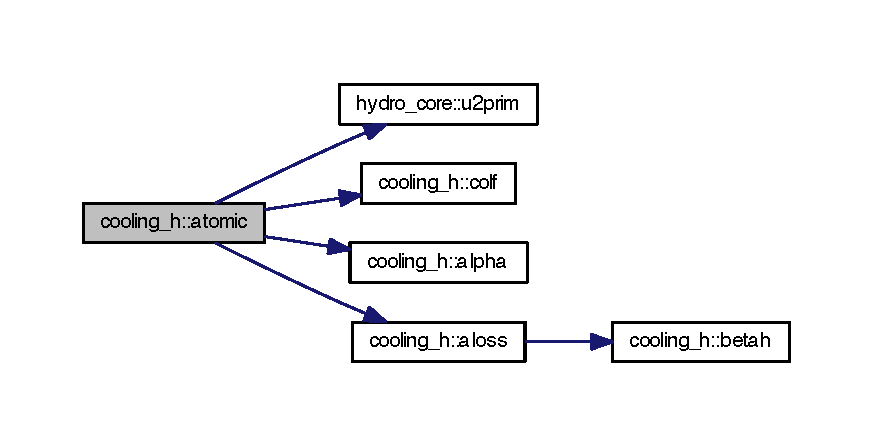
\includegraphics[width=350pt]{namespacecooling__h_aef95dbca5e7aef78d66a225cc217c982_cgraph}
\end{center}
\end{figure}


\hypertarget{namespacecooling__h_a2a2de25572bd515eae9441391e0ed0f8}{}\index{cooling\+\_\+h@{cooling\+\_\+h}!betah@{betah}}
\index{betah@{betah}!cooling\+\_\+h@{cooling\+\_\+h}}
\subsubsection[{betah}]{\setlength{\rightskip}{0pt plus 5cm}real (kind=8) function cooling\+\_\+h\+::betah (
\begin{DoxyParamCaption}
\item[{real (kind=8), intent(in)}]{T}
\end{DoxyParamCaption}
)}\label{namespacecooling__h_a2a2de25572bd515eae9441391e0ed0f8}
$ \beta_H(T) $ 
\begin{DoxyParams}{Parameters}
{\em real} & 8\mbox{[}in\mbox{]} T \+: Temperature K \\
\hline
\end{DoxyParams}


Definition at line 130 of file cooling\+\_\+h.\+f90.

\hypertarget{namespacecooling__h_ad5f1352f8925ccb1b352d6e749465a92}{}\index{cooling\+\_\+h@{cooling\+\_\+h}!colf@{colf}}
\index{colf@{colf}!cooling\+\_\+h@{cooling\+\_\+h}}
\subsubsection[{colf}]{\setlength{\rightskip}{0pt plus 5cm}real (kind=8) function cooling\+\_\+h\+::colf (
\begin{DoxyParamCaption}
\item[{real (kind=8), intent(in)}]{T}
\end{DoxyParamCaption}
)}\label{namespacecooling__h_ad5f1352f8925ccb1b352d6e749465a92}
calculates the collisional ionization rate 
\begin{DoxyParams}{Parameters}
{\em real8\mbox{[}in\mbox{]}} & T \+: Temperature K \\
\hline
\end{DoxyParams}


Definition at line 113 of file cooling\+\_\+h.\+f90.

\hypertarget{namespacecooling__h_aee85faa3b36e05a8efb05c1588f34ef2}{}\index{cooling\+\_\+h@{cooling\+\_\+h}!coolingh@{coolingh}}
\index{coolingh@{coolingh}!cooling\+\_\+h@{cooling\+\_\+h}}
\subsubsection[{coolingh}]{\setlength{\rightskip}{0pt plus 5cm}subroutine cooling\+\_\+h\+::coolingh (
\begin{DoxyParamCaption}
{}
\end{DoxyParamCaption}
)}\label{namespacecooling__h_aee85faa3b36e05a8efb05c1588f34ef2}
High level wrapper to apply cooling ~\newline
 parametrized cooling curve, uses the ionization state of hydrogen and ties the O I and I\+I to it 

Definition at line 42 of file cooling\+\_\+h.\+f90.



Here is the call graph for this function\+:
% FIG 0



\hypertarget{namespacedifrad}{}\section{difrad Module Reference}
\label{namespacedifrad}\index{difrad@{difrad}}


Ray tracing Radiative Trasnport.  


\subsection*{Functions/\+Subroutines}
\begin{DoxyCompactItemize}
\item 
subroutine \hyperlink{namespacedifrad_a9bce19025195159710828548c95282dc}{init\+\_\+rand} ()
\begin{DoxyCompactList}\small\item\em initializes random number generation \end{DoxyCompactList}\item 
subroutine \hyperlink{namespacedifrad_a1ccb144621689571d836f2f76c5fabae}{emdiff} (emax)
\begin{DoxyCompactList}\small\item\em calculates the diffuse fotoionization emissivity \end{DoxyCompactList}\item 
subroutine \hyperlink{namespacedifrad_ac7efbacd89420f5c298f7fb666ba14f9}{random\+\_\+versor} (xd, yd, zd)
\begin{DoxyCompactList}\small\item\em returns the 3 components of a random versor \end{DoxyCompactList}\item 
subroutine \hyperlink{namespacedifrad_a180fbbe2c9b0639cc33dd6ef57a61ec4}{starsource} (srad, x0, y0, z0, x, y, z, xd, yd, zd)
\begin{DoxyCompactList}\small\item\em Place photon packets at a \char`\"{}star\char`\"{} surface. \end{DoxyCompactList}\item 
subroutine \hyperlink{namespacedifrad_a39291c8aa2927c69ef6ca60f78c9b103}{photons} (xl0, yl0, zl0, xd, yd, zd, f)
\begin{DoxyCompactList}\small\item\em Photon trajectories. \end{DoxyCompactList}\item 
subroutine \hyperlink{namespacedifrad_afe6e9d2182e755ae483aeaa2c91f2710}{radbounds} ()
\begin{DoxyCompactList}\small\item\em follows the rays across M\+P\+I boundaries \end{DoxyCompactList}\item 
subroutine \hyperlink{namespacedifrad_a17151a5334db41fd14315d454e883b8e}{progress} (j, tot)
\begin{DoxyCompactList}\small\item\em Progress bar. \end{DoxyCompactList}\item 
subroutine \hyperlink{namespacedifrad_aeec1cd3dae50e6946aadb42abef934ec}{diffuse\+\_\+rad} ()
\begin{DoxyCompactList}\small\item\em Diffuse radiation driver. \end{DoxyCompactList}\end{DoxyCompactItemize}
\subsection*{Variables}
\begin{DoxyCompactItemize}
\item 
\hypertarget{namespacedifrad_a0062472e34b740c2c1cb5084d3284056}{}real, parameter \hyperlink{namespacedifrad_a0062472e34b740c2c1cb5084d3284056}{a0} =6.\+3e-\/18\label{namespacedifrad_a0062472e34b740c2c1cb5084d3284056}

\begin{DoxyCompactList}\small\item\em Fotoionization cross section. \end{DoxyCompactList}\item 
\hypertarget{namespacedifrad_aac6943b42d4dede95a3296bdc29c629a}{}integer, parameter \hyperlink{namespacedifrad_aac6943b42d4dede95a3296bdc29c629a}{nrays} =1000000\label{namespacedifrad_aac6943b42d4dede95a3296bdc29c629a}

\begin{DoxyCompactList}\small\item\em Number of rays. \end{DoxyCompactList}\item 
\hypertarget{namespacedifrad_ab532f1879434284f63aa97c79c305236}{}real, dimension(\+:,\+:,\+:), allocatable \hyperlink{namespacedifrad_ab532f1879434284f63aa97c79c305236}{ph}\label{namespacedifrad_ab532f1879434284f63aa97c79c305236}

\begin{DoxyCompactList}\small\item\em Photoionizing rate. \end{DoxyCompactList}\item 
\hypertarget{namespacedifrad_a7d908916fd1e050b9c5ba48771186d5b}{}real, dimension(\+:,\+:,\+:), allocatable \hyperlink{namespacedifrad_a7d908916fd1e050b9c5ba48771186d5b}{em}\label{namespacedifrad_a7d908916fd1e050b9c5ba48771186d5b}

\begin{DoxyCompactList}\small\item\em Photoionizing emissivity. \end{DoxyCompactList}\item 
\hypertarget{namespacedifrad_a3d6a043ec876c626f11238b6260a036a}{}real, dimension(\+:,\+:,\+:), allocatable \hyperlink{namespacedifrad_a3d6a043ec876c626f11238b6260a036a}{photl}\label{namespacedifrad_a3d6a043ec876c626f11238b6260a036a}

\begin{DoxyCompactList}\small\item\em Auxiliary buffer for M\+P\+I. \end{DoxyCompactList}\item 
\hypertarget{namespacedifrad_adf49e979d01582a3c0032f9bde3c4555}{}real, dimension(\+:,\+:,\+:), allocatable \hyperlink{namespacedifrad_adf49e979d01582a3c0032f9bde3c4555}{photr}\label{namespacedifrad_adf49e979d01582a3c0032f9bde3c4555}

\begin{DoxyCompactList}\small\item\em Auxiliary buffer for M\+P\+I. \end{DoxyCompactList}\item 
\hypertarget{namespacedifrad_a65e54816218f7e0acae4ffeaaf9523f6}{}real, dimension(\+:,\+:,\+:), allocatable \hyperlink{namespacedifrad_a65e54816218f7e0acae4ffeaaf9523f6}{photb}\label{namespacedifrad_a65e54816218f7e0acae4ffeaaf9523f6}

\begin{DoxyCompactList}\small\item\em Auxiliary buffer for M\+P\+I. \end{DoxyCompactList}\item 
\hypertarget{namespacedifrad_a28892e6d6f67cbcb8b65e79132cf959b}{}real, dimension(\+:,\+:,\+:), allocatable \hyperlink{namespacedifrad_a28892e6d6f67cbcb8b65e79132cf959b}{phott}\label{namespacedifrad_a28892e6d6f67cbcb8b65e79132cf959b}

\begin{DoxyCompactList}\small\item\em Auxiliary buffer for M\+P\+I. \end{DoxyCompactList}\item 
\hypertarget{namespacedifrad_a73a81002fda23212ff6d9d8b6d161f32}{}real, dimension(\+:,\+:,\+:), allocatable \hyperlink{namespacedifrad_a73a81002fda23212ff6d9d8b6d161f32}{photo}\label{namespacedifrad_a73a81002fda23212ff6d9d8b6d161f32}

\begin{DoxyCompactList}\small\item\em Auxiliary buffer for M\+P\+I. \end{DoxyCompactList}\item 
\hypertarget{namespacedifrad_afa84bdf37b43d72b3e3e3b3c6291807e}{}real, dimension(\+:,\+:,\+:), allocatable \hyperlink{namespacedifrad_afa84bdf37b43d72b3e3e3b3c6291807e}{photi}\label{namespacedifrad_afa84bdf37b43d72b3e3e3b3c6291807e}

\begin{DoxyCompactList}\small\item\em Auxiliary buffer for M\+P\+I. \end{DoxyCompactList}\item 
\hypertarget{namespacedifrad_a1d5243b742ea3504f1b6b09132417333}{}integer, dimension(6) \hyperlink{namespacedifrad_a1d5243b742ea3504f1b6b09132417333}{buffersize}\label{namespacedifrad_a1d5243b742ea3504f1b6b09132417333}

\begin{DoxyCompactList}\small\item\em Auxiliary buffer for M\+P\+I. \end{DoxyCompactList}\end{DoxyCompactItemize}


\subsection{Detailed Description}
Ray tracing Radiative Trasnport 

\subsection{Function/\+Subroutine Documentation}
\hypertarget{namespacedifrad_aeec1cd3dae50e6946aadb42abef934ec}{}\index{difrad@{difrad}!diffuse\+\_\+rad@{diffuse\+\_\+rad}}
\index{diffuse\+\_\+rad@{diffuse\+\_\+rad}!difrad@{difrad}}
\subsubsection[{diffuse\+\_\+rad}]{\setlength{\rightskip}{0pt plus 5cm}subroutine difrad\+::diffuse\+\_\+rad (
\begin{DoxyParamCaption}
{}
\end{DoxyParamCaption}
)}\label{namespacedifrad_aeec1cd3dae50e6946aadb42abef934ec}
Upper level wrapper to compute the diffuse photoionization rate 

Definition at line 655 of file difrad.\+f90.



Here is the call graph for this function\+:\nopagebreak
\begin{figure}[H]
\begin{center}
\leavevmode
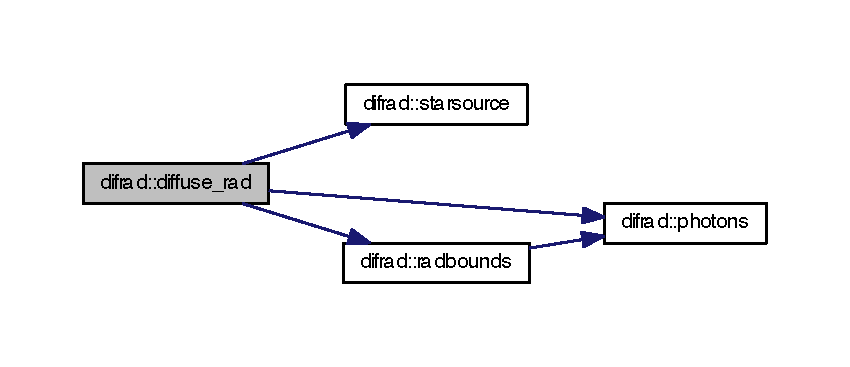
\includegraphics[width=350pt]{namespacedifrad_aeec1cd3dae50e6946aadb42abef934ec_cgraph}
\end{center}
\end{figure}


\hypertarget{namespacedifrad_a1ccb144621689571d836f2f76c5fabae}{}\index{difrad@{difrad}!emdiff@{emdiff}}
\index{emdiff@{emdiff}!difrad@{difrad}}
\subsubsection[{emdiff}]{\setlength{\rightskip}{0pt plus 5cm}subroutine difrad\+::emdiff (
\begin{DoxyParamCaption}
\item[{real, intent(out)}]{emax}
\end{DoxyParamCaption}
)}\label{namespacedifrad_a1ccb144621689571d836f2f76c5fabae}
calculates the diffuse fotoionization emissivity in the entire domain 
\begin{DoxyParams}{Parameters}
{\em real} & \mbox{[}out\mbox{]} emax \+: maximum emissivity in the entire grid \\
\hline
\end{DoxyParams}


Definition at line 98 of file difrad.\+f90.



Here is the call graph for this function\+:\nopagebreak
\begin{figure}[H]
\begin{center}
\leavevmode
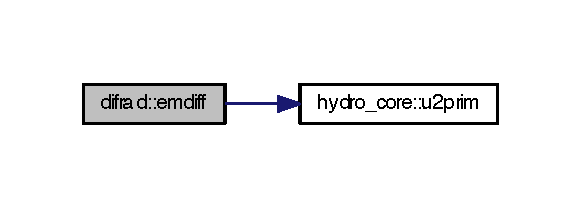
\includegraphics[width=293pt]{namespacedifrad_a1ccb144621689571d836f2f76c5fabae_cgraph}
\end{center}
\end{figure}


\hypertarget{namespacedifrad_a9bce19025195159710828548c95282dc}{}\index{difrad@{difrad}!init\+\_\+rand@{init\+\_\+rand}}
\index{init\+\_\+rand@{init\+\_\+rand}!difrad@{difrad}}
\subsubsection[{init\+\_\+rand}]{\setlength{\rightskip}{0pt plus 5cm}subroutine difrad\+::init\+\_\+rand (
\begin{DoxyParamCaption}
{}
\end{DoxyParamCaption}
)}\label{namespacedifrad_a9bce19025195159710828548c95282dc}
initializes random number generation 

Definition at line 56 of file difrad.\+f90.

\hypertarget{namespacedifrad_a39291c8aa2927c69ef6ca60f78c9b103}{}\index{difrad@{difrad}!photons@{photons}}
\index{photons@{photons}!difrad@{difrad}}
\subsubsection[{photons}]{\setlength{\rightskip}{0pt plus 5cm}subroutine difrad\+::photons (
\begin{DoxyParamCaption}
\item[{real, intent(in)}]{xl0, }
\item[{real, intent(in)}]{yl0, }
\item[{real, intent(in)}]{zl0, }
\item[{real, intent(in)}]{xd, }
\item[{real, intent(in)}]{yd, }
\item[{real, intent(in)}]{zd, }
\item[{real, intent(inout)}]{f}
\end{DoxyParamCaption}
)}\label{namespacedifrad_a39291c8aa2927c69ef6ca60f78c9b103}
Launches a photon from cell (xc,yc,zc) in the (xd,yd,zd) direction, with f and ionizing photons, and updates the photoionizing rate 
\begin{DoxyParams}{Parameters}
{\em real} & \mbox{[}in\mbox{]} xl0 \+: Initial X position \\
\hline
{\em real} & \mbox{[}in\mbox{]} yl0 \+: Initial Y position \\
\hline
{\em real} & \mbox{[}in\mbox{]} zl0 \+: Initial Z position \\
\hline
{\em real} & \mbox{[}in\mbox{]} xd \+: Direction in X \\
\hline
{\em real} & \mbox{[}in\mbox{]} yd \+: Direction in Y \\
\hline
{\em real} & \mbox{[}in\mbox{]} zd \+: Direction in Z \\
\hline
{\em real} & \mbox{[}in\mbox{]} f \+: N\+Umber of photoionizong photons \\
\hline
\end{DoxyParams}


Definition at line 252 of file difrad.\+f90.

\hypertarget{namespacedifrad_a17151a5334db41fd14315d454e883b8e}{}\index{difrad@{difrad}!progress@{progress}}
\index{progress@{progress}!difrad@{difrad}}
\subsubsection[{progress}]{\setlength{\rightskip}{0pt plus 5cm}subroutine difrad\+::progress (
\begin{DoxyParamCaption}
\item[{integer(kind=4)}]{j, }
\item[{integer(kind=4), intent(in)}]{tot}
\end{DoxyParamCaption}
)}\label{namespacedifrad_a17151a5334db41fd14315d454e883b8e}
Progress bar (only tested with Fortran conmpiler) takes a number between 1 and tot 
\begin{DoxyParams}{Parameters}
{\em integer} & \mbox{[}in\mbox{]} j \+: current iteration \\
\hline
{\em integer} & \mbox{[}in\mbox{]} tot \+: total number of iterartions \\
\hline
\end{DoxyParams}


Definition at line 633 of file difrad.\+f90.

\hypertarget{namespacedifrad_afe6e9d2182e755ae483aeaa2c91f2710}{}\index{difrad@{difrad}!radbounds@{radbounds}}
\index{radbounds@{radbounds}!difrad@{difrad}}
\subsubsection[{radbounds}]{\setlength{\rightskip}{0pt plus 5cm}subroutine difrad\+::radbounds (
\begin{DoxyParamCaption}
{}
\end{DoxyParamCaption}
)}\label{namespacedifrad_afe6e9d2182e755ae483aeaa2c91f2710}
follows the rays across M\+P\+I boundaries 

Definition at line 455 of file difrad.\+f90.



Here is the call graph for this function\+:\nopagebreak
\begin{figure}[H]
\begin{center}
\leavevmode
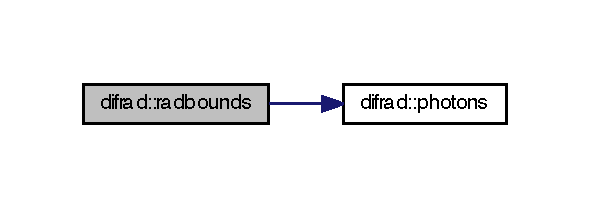
\includegraphics[width=293pt]{namespacedifrad_afe6e9d2182e755ae483aeaa2c91f2710_cgraph}
\end{center}
\end{figure}


\hypertarget{namespacedifrad_ac7efbacd89420f5c298f7fb666ba14f9}{}\index{difrad@{difrad}!random\+\_\+versor@{random\+\_\+versor}}
\index{random\+\_\+versor@{random\+\_\+versor}!difrad@{difrad}}
\subsubsection[{random\+\_\+versor}]{\setlength{\rightskip}{0pt plus 5cm}subroutine difrad\+::random\+\_\+versor (
\begin{DoxyParamCaption}
\item[{real, intent(out)}]{xd, }
\item[{real, intent(out)}]{yd, }
\item[{real, intent(out)}]{zd}
\end{DoxyParamCaption}
)}\label{namespacedifrad_ac7efbacd89420f5c298f7fb666ba14f9}
returns the 3 components of a random versor (unit magnitude) 
\begin{DoxyParams}{Parameters}
{\em real} & \mbox{[}out\mbox{]} xd \+: x component \\
\hline
{\em real} & \mbox{[}out\mbox{]} yd \+: y component \\
\hline
{\em real} & \mbox{[}out\mbox{]} zd \+: z component \\
\hline
\end{DoxyParams}


Definition at line 149 of file difrad.\+f90.

\hypertarget{namespacedifrad_a180fbbe2c9b0639cc33dd6ef57a61ec4}{}\index{difrad@{difrad}!starsource@{starsource}}
\index{starsource@{starsource}!difrad@{difrad}}
\subsubsection[{starsource}]{\setlength{\rightskip}{0pt plus 5cm}subroutine difrad\+::starsource (
\begin{DoxyParamCaption}
\item[{real, intent(in)}]{srad, }
\item[{real, intent(in)}]{x0, }
\item[{real, intent(in)}]{y0, }
\item[{real, intent(in)}]{z0, }
\item[{real, intent(out)}]{x, }
\item[{real, intent(out)}]{y, }
\item[{real, intent(out)}]{z, }
\item[{real, intent(out)}]{xd, }
\item[{real, intent(out)}]{yd, }
\item[{real, intent(out)}]{zd}
\end{DoxyParamCaption}
)}\label{namespacedifrad_a180fbbe2c9b0639cc33dd6ef57a61ec4}
returns the random location and direction at a star surface, if the direction goes into the star, the direction is inverted 
\begin{DoxyParams}{Parameters}
{\em real} & \mbox{[}in\mbox{]} Srad \+: radius of the \char`\"{}star\char`\"{} \\
\hline
{\em real} & \mbox{[}in\mbox{]} x0 \+: X position of the center of the star \\
\hline
{\em real} & \mbox{[}in\mbox{]} y0 \+: Y position of the center of the star \\
\hline
{\em real} & \mbox{[}in\mbox{]} y0 \+: Z position of the center of the star \\
\hline
{\em real} & \mbox{[}out\mbox{]} x \+: random X position at the star surface \\
\hline
{\em real} & \mbox{[}out\mbox{]} y \+: random Y position at the star surface \\
\hline
{\em real} & \mbox{[}out\mbox{]} z \+: random Z position at the star surface \\
\hline
{\em real} & \mbox{[}out\mbox{]} xd \+: random X direction \\
\hline
{\em real} & \mbox{[}out\mbox{]} yd \+: random Y direction \\
\hline
{\em real} & \mbox{[}out\mbox{]} zd \+: random Z direction \\
\hline
\end{DoxyParams}


Definition at line 187 of file difrad.\+f90.


\hypertarget{namespaceglobals}{}\section{globals Module Reference}
\label{namespaceglobals}\index{globals@{globals}}


Module containing global variables.  


\subsection*{Variables}
\begin{DoxyCompactItemize}
\item 
\hypertarget{namespaceglobals_ae6519b751f8ef608c2074e27024335b7}{}real, dimension(\+:,\+:,\+:,\+:), allocatable \hyperlink{namespaceglobals_ae6519b751f8ef608c2074e27024335b7}{u}\label{namespaceglobals_ae6519b751f8ef608c2074e27024335b7}

\begin{DoxyCompactList}\small\item\em conserved varibles \end{DoxyCompactList}\item 
\hypertarget{namespaceglobals_a127abb71c460a346ae47d10d86c22cc9}{}real, dimension(\+:,\+:,\+:,\+:), allocatable \hyperlink{namespaceglobals_a127abb71c460a346ae47d10d86c22cc9}{up}\label{namespaceglobals_a127abb71c460a346ae47d10d86c22cc9}

\begin{DoxyCompactList}\small\item\em conserved varibles after 1/2 timestep \end{DoxyCompactList}\item 
\hypertarget{namespaceglobals_a149bece4e7407071629f69a8c7deb03a}{}real, dimension(\+:,\+:,\+:,\+:), allocatable \hyperlink{namespaceglobals_a149bece4e7407071629f69a8c7deb03a}{primit}\label{namespaceglobals_a149bece4e7407071629f69a8c7deb03a}

\begin{DoxyCompactList}\small\item\em primitive varibles \end{DoxyCompactList}\item 
\hypertarget{namespaceglobals_a5fb85172ca54e822fdb8c522da890717}{}real, dimension(\+:,\+:,\+:,\+:), allocatable \hyperlink{namespaceglobals_a5fb85172ca54e822fdb8c522da890717}{f}\label{namespaceglobals_a5fb85172ca54e822fdb8c522da890717}

\begin{DoxyCompactList}\small\item\em X fluxes. \end{DoxyCompactList}\item 
\hypertarget{namespaceglobals_a0124c44fda4a3092edd2789f79dec648}{}real, dimension(\+:,\+:,\+:,\+:), allocatable \hyperlink{namespaceglobals_a0124c44fda4a3092edd2789f79dec648}{g}\label{namespaceglobals_a0124c44fda4a3092edd2789f79dec648}

\begin{DoxyCompactList}\small\item\em Y fluxes. \end{DoxyCompactList}\item 
\hypertarget{namespaceglobals_af6262d058b86075848725c846e7cc9cc}{}real, dimension(\+:,\+:,\+:,\+:), allocatable \hyperlink{namespaceglobals_af6262d058b86075848725c846e7cc9cc}{h}\label{namespaceglobals_af6262d058b86075848725c846e7cc9cc}

\begin{DoxyCompactList}\small\item\em Z fluxes. \end{DoxyCompactList}\item 
\hypertarget{namespaceglobals_aafee650389fdf595e41e37cb340155ae}{}real \hyperlink{namespaceglobals_aafee650389fdf595e41e37cb340155ae}{dx}\label{namespaceglobals_aafee650389fdf595e41e37cb340155ae}

\begin{DoxyCompactList}\small\item\em grid spacing in X \end{DoxyCompactList}\item 
\hypertarget{namespaceglobals_a9b12323045a0672fe06f9b7091cd3e7a}{}real \hyperlink{namespaceglobals_a9b12323045a0672fe06f9b7091cd3e7a}{dy}\label{namespaceglobals_a9b12323045a0672fe06f9b7091cd3e7a}

\begin{DoxyCompactList}\small\item\em grid spacing in Y \end{DoxyCompactList}\item 
\hypertarget{namespaceglobals_a81293f145f1af171eb88b6feced78c95}{}real \hyperlink{namespaceglobals_a81293f145f1af171eb88b6feced78c95}{dz}\label{namespaceglobals_a81293f145f1af171eb88b6feced78c95}

\begin{DoxyCompactList}\small\item\em grid spacing in Z \end{DoxyCompactList}\item 
\hypertarget{namespaceglobals_a8d38eca539ad2b24a66616e42b79ac4c}{}integer, dimension(0\+:2) \hyperlink{namespaceglobals_a8d38eca539ad2b24a66616e42b79ac4c}{coords}\label{namespaceglobals_a8d38eca539ad2b24a66616e42b79ac4c}

\begin{DoxyCompactList}\small\item\em position of neighboring M\+P\+I blocks \end{DoxyCompactList}\item 
\hypertarget{namespaceglobals_aba9a16c1b0ed3e52dce83157476d099c}{}integer \hyperlink{namespaceglobals_aba9a16c1b0ed3e52dce83157476d099c}{left}\label{namespaceglobals_aba9a16c1b0ed3e52dce83157476d099c}

\begin{DoxyCompactList}\small\item\em M\+P\+I neighbor in the -\/x direction. \end{DoxyCompactList}\item 
\hypertarget{namespaceglobals_a0b27e5c90473860434fc5dd58a255111}{}integer \hyperlink{namespaceglobals_a0b27e5c90473860434fc5dd58a255111}{right}\label{namespaceglobals_a0b27e5c90473860434fc5dd58a255111}

\begin{DoxyCompactList}\small\item\em M\+P\+I neighbor in the +x direction. \end{DoxyCompactList}\item 
\hypertarget{namespaceglobals_add36bccef8d272ff40330a62d0307580}{}integer \hyperlink{namespaceglobals_add36bccef8d272ff40330a62d0307580}{top}\label{namespaceglobals_add36bccef8d272ff40330a62d0307580}

\begin{DoxyCompactList}\small\item\em M\+P\+I neighbor in the -\/y direction. \end{DoxyCompactList}\item 
\hypertarget{namespaceglobals_a3188a89193263f9f063099801321d525}{}integer \hyperlink{namespaceglobals_a3188a89193263f9f063099801321d525}{bottom}\label{namespaceglobals_a3188a89193263f9f063099801321d525}

\begin{DoxyCompactList}\small\item\em M\+P\+I neighbor in the +y direction. \end{DoxyCompactList}\item 
\hypertarget{namespaceglobals_ac3375149d8b96b3b5470274034850ecc}{}integer \hyperlink{namespaceglobals_ac3375149d8b96b3b5470274034850ecc}{out}\label{namespaceglobals_ac3375149d8b96b3b5470274034850ecc}

\begin{DoxyCompactList}\small\item\em M\+P\+I neighbor in the -\/z direction. \end{DoxyCompactList}\item 
\hypertarget{namespaceglobals_a6a2cc973507c2f9ea75f44a9f976d659}{}integer \hyperlink{namespaceglobals_a6a2cc973507c2f9ea75f44a9f976d659}{in}\label{namespaceglobals_a6a2cc973507c2f9ea75f44a9f976d659}

\begin{DoxyCompactList}\small\item\em M\+P\+I neighbor in the +z direction. \end{DoxyCompactList}\item 
\hypertarget{namespaceglobals_a93f283242b146b3ef8b53fd1b1ad7bac}{}integer \hyperlink{namespaceglobals_a93f283242b146b3ef8b53fd1b1ad7bac}{rank}\label{namespaceglobals_a93f283242b146b3ef8b53fd1b1ad7bac}

\begin{DoxyCompactList}\small\item\em M\+P\+I rank. \end{DoxyCompactList}\item 
\hypertarget{namespaceglobals_a4bc8f1b5670efd802d57dce2c385b6d9}{}integer \hyperlink{namespaceglobals_a4bc8f1b5670efd802d57dce2c385b6d9}{comm3d}\label{namespaceglobals_a4bc8f1b5670efd802d57dce2c385b6d9}

\begin{DoxyCompactList}\small\item\em Cartessian M\+P\+I comunicator. \end{DoxyCompactList}\end{DoxyCompactItemize}


\subsection{Detailed Description}
This mudules contains variables that are treated as global in the code 
\hypertarget{namespaceh__alpha__utilities}{}\section{h\+\_\+alpha\+\_\+utilities Module Reference}
\label{namespaceh__alpha__utilities}\index{h\+\_\+alpha\+\_\+utilities@{h\+\_\+alpha\+\_\+utilities}}


H alpha projection.  


\subsection*{Functions/\+Subroutines}
\begin{DoxyCompactItemize}
\item 
subroutine \hyperlink{namespaceh__alpha__utilities_a8bb4ef22ad133f8d3f75cf1a26e14035}{init\+\_\+ha} ()
\begin{DoxyCompactList}\small\item\em Initializes data. \end{DoxyCompactList}\item 
subroutine \hyperlink{namespaceh__alpha__utilities_a5549bf9fd812d02d9189d27f380c01c0}{read\+\_\+data} (u, itprint, filepath)
\begin{DoxyCompactList}\small\item\em reads data from file \end{DoxyCompactList}\item 
subroutine \hyperlink{namespaceh__alpha__utilities_af48cd3c223c292170bc1f90da256f537}{getxyz} (i, j, k, x, y, z)
\begin{DoxyCompactList}\small\item\em gets position of a cell \end{DoxyCompactList}\item 
subroutine \hyperlink{namespaceh__alpha__utilities_a65ad5d15c1265e31f4d191ebf771e669}{rotation\+\_\+x} (theta, x, y, z, xn, yn, zn)
\begin{DoxyCompactList}\small\item\em Rotation around the X axis. \end{DoxyCompactList}\item 
subroutine \hyperlink{namespaceh__alpha__utilities_ab643f1bac838912c58b25923b5de40ca}{rotation\+\_\+y} (theta, x, y, z, xn, yn, zn)
\begin{DoxyCompactList}\small\item\em Rotation around the Y axis. \end{DoxyCompactList}\item 
subroutine \hyperlink{namespaceh__alpha__utilities_acaf25f2c0ad80c5d7e2f451f58522a49}{rotation\+\_\+z} (theta, x, y, z, xn, yn, zn)
\begin{DoxyCompactList}\small\item\em Rotation around the Z axis. \end{DoxyCompactList}\item 
subroutine \hyperlink{namespaceh__alpha__utilities_aafc5cae88b562d0bd2d039cae21ed35a}{fill\+\_\+map} (nxmap, nymap, u, map, dx\+T, dy\+T, theta\+\_\+x, theta\+\_\+y, theta\+\_\+z)
\begin{DoxyCompactList}\small\item\em Fill target map. \end{DoxyCompactList}\item 
subroutine \hyperlink{namespaceh__alpha__utilities_aa2b2b3783ef4b30d178412ea44671047}{write\+\_\+ha} (fileout, nxmap, nymap, map)
\begin{DoxyCompactList}\small\item\em Writes projection to file. \end{DoxyCompactList}\item 
subroutine \hyperlink{namespaceh__alpha__utilities_a1cf6b2b4be1a68c792b3cb07b5629af6}{write\+\_\+rg} (fileout, nxmap, nymap, map)
\begin{DoxyCompactList}\small\item\em Writes projection to file in rg format. \end{DoxyCompactList}\end{DoxyCompactItemize}


\subsection{Detailed Description}
Utilities to compute an H alpha map 

\subsection{Function/\+Subroutine Documentation}
\hypertarget{namespaceh__alpha__utilities_aafc5cae88b562d0bd2d039cae21ed35a}{}\index{h\+\_\+alpha\+\_\+utilities@{h\+\_\+alpha\+\_\+utilities}!fill\+\_\+map@{fill\+\_\+map}}
\index{fill\+\_\+map@{fill\+\_\+map}!h\+\_\+alpha\+\_\+utilities@{h\+\_\+alpha\+\_\+utilities}}
\subsubsection[{fill\+\_\+map}]{\setlength{\rightskip}{0pt plus 5cm}subroutine h\+\_\+alpha\+\_\+utilities\+::fill\+\_\+map (
\begin{DoxyParamCaption}
\item[{integer, intent(in)}]{nxmap, }
\item[{integer, intent(in)}]{nymap, }
\item[{real, dimension(neq,nxmin\+:nxmax,nymin\+:nymax, nzmin\+:nzmax), intent(in)}]{u, }
\item[{real, dimension(nxmap,nymap), intent(out)}]{map, }
\item[{real, intent(in)}]{dx\+T, }
\item[{real, intent(in)}]{dy\+T, }
\item[{real, intent(in)}]{theta\+\_\+x, }
\item[{real, intent(in)}]{theta\+\_\+y, }
\item[{real, intent(in)}]{theta\+\_\+z}
\end{DoxyParamCaption}
)}\label{namespaceh__alpha__utilities_aafc5cae88b562d0bd2d039cae21ed35a}
Fills the target map of one M\+P\+I block 
\begin{DoxyParams}{Parameters}
{\em integer} & \mbox{[}in\mbox{]} nxmap \+: Number of X cells in target \\
\hline
{\em integer} & \mbox{[}in\mbox{]} nymap \+: Number of Y cells in target \\
\hline
{\em real} & \mbox{[}in\mbox{]} u(neq,nxmin\+:nxmax,nymin\+:nymax, nzmin\+:nzmax) \+: conserved variables \\
\hline
{\em real} & \mbox{[}out\mbox{]} map(nxmap,mymap) \+: Target map \\
\hline
{\em real} & \mbox{[}in\mbox{]} dx\+T \+: target pixel width \\
\hline
{\em real} & \mbox{[}in\mbox{]} dy\+T \+: target pixel height \\
\hline
{\em real} & \mbox{[}in\mbox{]} thetax \+: Rotation around X \\
\hline
{\em real} & \mbox{[}in\mbox{]} thetay \+: Rotation around Y \\
\hline
{\em real} & \mbox{[}in\mbox{]} thetaz \+: Rotation around Z \\
\hline
\end{DoxyParams}


Definition at line 285 of file h\+\_\+alpha\+\_\+proj.\+f90.



Here is the call graph for this function\+:\nopagebreak
\begin{figure}[H]
\begin{center}
\leavevmode
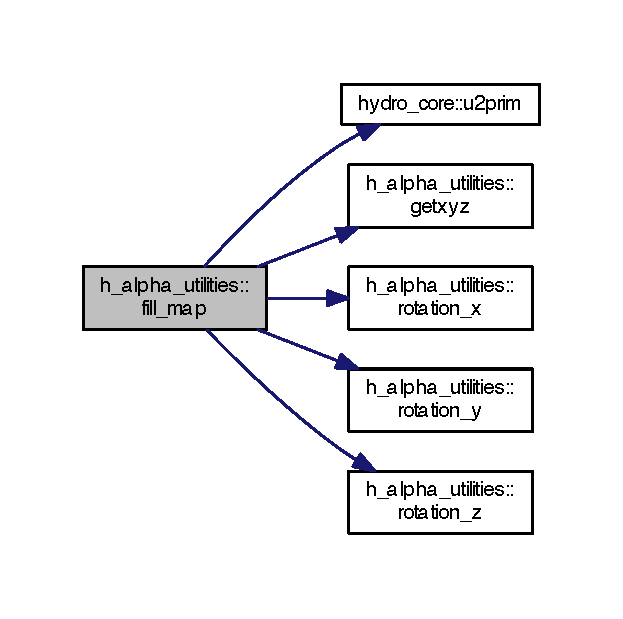
\includegraphics[width=313pt]{namespaceh__alpha__utilities_aafc5cae88b562d0bd2d039cae21ed35a_cgraph}
\end{center}
\end{figure}


\hypertarget{namespaceh__alpha__utilities_af48cd3c223c292170bc1f90da256f537}{}\index{h\+\_\+alpha\+\_\+utilities@{h\+\_\+alpha\+\_\+utilities}!getxyz@{getxyz}}
\index{getxyz@{getxyz}!h\+\_\+alpha\+\_\+utilities@{h\+\_\+alpha\+\_\+utilities}}
\subsubsection[{getxyz}]{\setlength{\rightskip}{0pt plus 5cm}subroutine h\+\_\+alpha\+\_\+utilities\+::getxyz (
\begin{DoxyParamCaption}
\item[{integer, intent(in)}]{i, }
\item[{integer, intent(in)}]{j, }
\item[{integer, intent(in)}]{k, }
\item[{real, intent(out)}]{x, }
\item[{real, intent(out)}]{y, }
\item[{real, intent(out)}]{z}
\end{DoxyParamCaption}
)}\label{namespaceh__alpha__utilities_af48cd3c223c292170bc1f90da256f537}
Returns the position and spherical radius calculated with respect to the center of the grid 
\begin{DoxyParams}{Parameters}
{\em integer} & \mbox{[}in\mbox{]} i \+: cell index in the x direction \\
\hline
{\em integer} & \mbox{[}in\mbox{]} j \+: cell index in the y direction \\
\hline
{\em integer} & \mbox{[}in\mbox{]} k \+: cell index in the z direction \\
\hline
{\em real} & \mbox{[}in\mbox{]} x \+: x position in the grid \\
\hline
{\em real} & \mbox{[}in\mbox{]} y \+: y position in the grid \\
\hline
{\em real} & \mbox{[}in\mbox{]} z \+: z position in the grid \\
\hline
\end{DoxyParams}


Definition at line 187 of file h\+\_\+alpha\+\_\+proj.\+f90.

\hypertarget{namespaceh__alpha__utilities_a8bb4ef22ad133f8d3f75cf1a26e14035}{}\index{h\+\_\+alpha\+\_\+utilities@{h\+\_\+alpha\+\_\+utilities}!init\+\_\+ha@{init\+\_\+ha}}
\index{init\+\_\+ha@{init\+\_\+ha}!h\+\_\+alpha\+\_\+utilities@{h\+\_\+alpha\+\_\+utilities}}
\subsubsection[{init\+\_\+ha}]{\setlength{\rightskip}{0pt plus 5cm}subroutine h\+\_\+alpha\+\_\+utilities\+::init\+\_\+ha (
\begin{DoxyParamCaption}
{}
\end{DoxyParamCaption}
)}\label{namespaceh__alpha__utilities_a8bb4ef22ad133f8d3f75cf1a26e14035}
Initializes data, M\+P\+I and other stuff 

Definition at line 35 of file h\+\_\+alpha\+\_\+proj.\+f90.

\hypertarget{namespaceh__alpha__utilities_a5549bf9fd812d02d9189d27f380c01c0}{}\index{h\+\_\+alpha\+\_\+utilities@{h\+\_\+alpha\+\_\+utilities}!read\+\_\+data@{read\+\_\+data}}
\index{read\+\_\+data@{read\+\_\+data}!h\+\_\+alpha\+\_\+utilities@{h\+\_\+alpha\+\_\+utilities}}
\subsubsection[{read\+\_\+data}]{\setlength{\rightskip}{0pt plus 5cm}subroutine h\+\_\+alpha\+\_\+utilities\+::read\+\_\+data (
\begin{DoxyParamCaption}
\item[{real, dimension(neq,nxmin\+:nxmax,nymin\+:nymax,nzmin\+:nzmax), intent(out)}]{u, }
\item[{integer, intent(in)}]{itprint, }
\item[{character (len=128), intent(in)}]{filepath}
\end{DoxyParamCaption}
)}\label{namespaceh__alpha__utilities_a5549bf9fd812d02d9189d27f380c01c0}
reads data from file 
\begin{DoxyParams}{Parameters}
{\em real} & \mbox{[}out\mbox{]} u(neq,nxmin\+:nxmax,nymin\+:nymax,nzmin\+:nzmax) \+: conserved variables \\
\hline
{\em integer} & \mbox{[}in\mbox{]} itprint \+: number of output \\
\hline
{\em string} & \mbox{[}in\mbox{]} filepath \+: path where the output is \\
\hline
\end{DoxyParams}


Definition at line 134 of file h\+\_\+alpha\+\_\+proj.\+f90.

\hypertarget{namespaceh__alpha__utilities_a65ad5d15c1265e31f4d191ebf771e669}{}\index{h\+\_\+alpha\+\_\+utilities@{h\+\_\+alpha\+\_\+utilities}!rotation\+\_\+x@{rotation\+\_\+x}}
\index{rotation\+\_\+x@{rotation\+\_\+x}!h\+\_\+alpha\+\_\+utilities@{h\+\_\+alpha\+\_\+utilities}}
\subsubsection[{rotation\+\_\+x}]{\setlength{\rightskip}{0pt plus 5cm}subroutine h\+\_\+alpha\+\_\+utilities\+::rotation\+\_\+x (
\begin{DoxyParamCaption}
\item[{real, intent(in)}]{theta, }
\item[{real, intent(in)}]{x, }
\item[{real, intent(in)}]{y, }
\item[{real, intent(in)}]{z, }
\item[{real, intent(out)}]{xn, }
\item[{real, intent(out)}]{yn, }
\item[{real, intent(out)}]{zn}
\end{DoxyParamCaption}
)}\label{namespaceh__alpha__utilities_a65ad5d15c1265e31f4d191ebf771e669}
Does a rotation around the x axis 
\begin{DoxyParams}{Parameters}
{\em real} & \mbox{[}in\mbox{]}, theta \+: Angle of rotation (in radians) \\
\hline
{\em real} & \mbox{[}in\mbox{]}, x \+: original x position in the grid \\
\hline
{\em real} & \mbox{[}in\mbox{]}, y \+: original y position in the grid \\
\hline
{\em real} & \mbox{[}in\mbox{]}, x \+: original z position in the grid \\
\hline
{\em real} & \mbox{[}out\mbox{]}, x \+: final x position in the grid \\
\hline
{\em real} & \mbox{[}out\mbox{]}, y \+: final y position in the grid \\
\hline
{\em real} & \mbox{[}out\mbox{]}, x \+: final z position in the grid \\
\hline
\end{DoxyParams}


Definition at line 213 of file h\+\_\+alpha\+\_\+proj.\+f90.

\hypertarget{namespaceh__alpha__utilities_ab643f1bac838912c58b25923b5de40ca}{}\index{h\+\_\+alpha\+\_\+utilities@{h\+\_\+alpha\+\_\+utilities}!rotation\+\_\+y@{rotation\+\_\+y}}
\index{rotation\+\_\+y@{rotation\+\_\+y}!h\+\_\+alpha\+\_\+utilities@{h\+\_\+alpha\+\_\+utilities}}
\subsubsection[{rotation\+\_\+y}]{\setlength{\rightskip}{0pt plus 5cm}subroutine h\+\_\+alpha\+\_\+utilities\+::rotation\+\_\+y (
\begin{DoxyParamCaption}
\item[{real, intent(in)}]{theta, }
\item[{real, intent(in)}]{x, }
\item[{real, intent(in)}]{y, }
\item[{real, intent(in)}]{z, }
\item[{real, intent(out)}]{xn, }
\item[{real, intent(out)}]{yn, }
\item[{real, intent(out)}]{zn}
\end{DoxyParamCaption}
)}\label{namespaceh__alpha__utilities_ab643f1bac838912c58b25923b5de40ca}
Does a rotation around the x axis 
\begin{DoxyParams}{Parameters}
{\em real} & \mbox{[}in\mbox{]}, theta \+: Angle of rotation (in radians) \\
\hline
{\em real} & \mbox{[}in\mbox{]}, x \+: original x position in the grid \\
\hline
{\em real} & \mbox{[}in\mbox{]}, y \+: original y position in the grid \\
\hline
{\em real} & \mbox{[}in\mbox{]}, x \+: original z position in the grid \\
\hline
{\em real} & \mbox{[}out\mbox{]}, x \+: final x position in the grid \\
\hline
{\em real} & \mbox{[}out\mbox{]}, y \+: final y position in the grid \\
\hline
{\em real} & \mbox{[}out\mbox{]}, x \+: final z position in the grid \\
\hline
\end{DoxyParams}


Definition at line 237 of file h\+\_\+alpha\+\_\+proj.\+f90.

\hypertarget{namespaceh__alpha__utilities_acaf25f2c0ad80c5d7e2f451f58522a49}{}\index{h\+\_\+alpha\+\_\+utilities@{h\+\_\+alpha\+\_\+utilities}!rotation\+\_\+z@{rotation\+\_\+z}}
\index{rotation\+\_\+z@{rotation\+\_\+z}!h\+\_\+alpha\+\_\+utilities@{h\+\_\+alpha\+\_\+utilities}}
\subsubsection[{rotation\+\_\+z}]{\setlength{\rightskip}{0pt plus 5cm}subroutine h\+\_\+alpha\+\_\+utilities\+::rotation\+\_\+z (
\begin{DoxyParamCaption}
\item[{real, intent(in)}]{theta, }
\item[{real, intent(in)}]{x, }
\item[{real, intent(in)}]{y, }
\item[{real, intent(in)}]{z, }
\item[{real, intent(out)}]{xn, }
\item[{real, intent(out)}]{yn, }
\item[{real, intent(out)}]{zn}
\end{DoxyParamCaption}
)}\label{namespaceh__alpha__utilities_acaf25f2c0ad80c5d7e2f451f58522a49}
Does a rotation around the x axis 
\begin{DoxyParams}{Parameters}
{\em real} & \mbox{[}in\mbox{]}, theta \+: Angle of rotation (in radians) \\
\hline
{\em real} & \mbox{[}in\mbox{]}, x \+: original x position in the grid \\
\hline
{\em real} & \mbox{[}in\mbox{]}, y \+: original y position in the grid \\
\hline
{\em real} & \mbox{[}in\mbox{]}, x \+: original z position in the grid \\
\hline
{\em real} & \mbox{[}out\mbox{]}, x \+: final x position in the grid \\
\hline
{\em real} & \mbox{[}out\mbox{]}, y \+: final y position in the grid \\
\hline
{\em real} & \mbox{[}out\mbox{]}, x \+: final z position in the grid \\
\hline
\end{DoxyParams}


Definition at line 259 of file h\+\_\+alpha\+\_\+proj.\+f90.

\hypertarget{namespaceh__alpha__utilities_aa2b2b3783ef4b30d178412ea44671047}{}\index{h\+\_\+alpha\+\_\+utilities@{h\+\_\+alpha\+\_\+utilities}!write\+\_\+ha@{write\+\_\+ha}}
\index{write\+\_\+ha@{write\+\_\+ha}!h\+\_\+alpha\+\_\+utilities@{h\+\_\+alpha\+\_\+utilities}}
\subsubsection[{write\+\_\+ha}]{\setlength{\rightskip}{0pt plus 5cm}subroutine h\+\_\+alpha\+\_\+utilities\+::write\+\_\+ha (
\begin{DoxyParamCaption}
\item[{character (len=128), intent(in)}]{fileout, }
\item[{integer, intent(in)}]{nxmap, }
\item[{integer, intent(in)}]{nymap, }
\item[{real, dimension(nxmap,nymap), intent(in)}]{map}
\end{DoxyParamCaption}
)}\label{namespaceh__alpha__utilities_aa2b2b3783ef4b30d178412ea44671047}
Writes projection to file 
\begin{DoxyParams}{Parameters}
{\em integer} & \mbox{[}in\mbox{]} itprint \+: number of output \\
\hline
{\em string} & \mbox{[}in\mbox{]} fileout \+: file where to write \\
\hline
{\em integer} & \mbox{[}in\mbox{]} nxmap \+: Number of X cells in target \\
\hline
{\em integer} & \mbox{[}in\mbox{]} nymap \+: Number of Y cells in target \\
\hline
{\em real} & \mbox{[}in\mbox{]} map(nxmap,mymap) \+: Target map \\
\hline
\end{DoxyParams}


Definition at line 362 of file h\+\_\+alpha\+\_\+proj.\+f90.

\hypertarget{namespaceh__alpha__utilities_a1cf6b2b4be1a68c792b3cb07b5629af6}{}\index{h\+\_\+alpha\+\_\+utilities@{h\+\_\+alpha\+\_\+utilities}!write\+\_\+rg@{write\+\_\+rg}}
\index{write\+\_\+rg@{write\+\_\+rg}!h\+\_\+alpha\+\_\+utilities@{h\+\_\+alpha\+\_\+utilities}}
\subsubsection[{write\+\_\+rg}]{\setlength{\rightskip}{0pt plus 5cm}subroutine h\+\_\+alpha\+\_\+utilities\+::write\+\_\+rg (
\begin{DoxyParamCaption}
\item[{character (len=128), intent(in)}]{fileout, }
\item[{integer, intent(in)}]{nxmap, }
\item[{integer, intent(in)}]{nymap, }
\item[{real, dimension(nxmap,nymap), intent(in)}]{map}
\end{DoxyParamCaption}
)}\label{namespaceh__alpha__utilities_a1cf6b2b4be1a68c792b3cb07b5629af6}
Writes projection to file 
\begin{DoxyParams}{Parameters}
{\em integer} & \mbox{[}in\mbox{]} itprint \+: number of output \\
\hline
{\em string} & \mbox{[}in\mbox{]} fileout \+: file where to write \\
\hline
{\em integer} & \mbox{[}in\mbox{]} nxmap \+: Number of X cells in target \\
\hline
{\em integer} & \mbox{[}in\mbox{]} nymap \+: Number of Y cells in target \\
\hline
{\em real} & \mbox{[}in\mbox{]} map(nxmap,mymap) \+: Target map \\
\hline
\end{DoxyParams}


Definition at line 391 of file h\+\_\+alpha\+\_\+proj.\+f90.


\hypertarget{namespacehll}{}\section{hll Module Reference}
\label{namespacehll}\index{hll@{hll}}


H\+L\+L approximate Riemann solver module.  


\subsection*{Functions/\+Subroutines}
\begin{DoxyCompactItemize}
\item 
subroutine \hyperlink{namespacehll_aa67c7db7e17f7dedf7286320baeda1dd}{prim2fhll} (priml, primr, ff)
\begin{DoxyCompactList}\small\item\em Solves the Riemann problem at the interface P\+L,P\+R using the H\+L\+L solver. \end{DoxyCompactList}\item 
subroutine \hyperlink{namespacehll_a27386fb5bcf705be5e8c2650484966c6}{hllfluxes} (choice)
\begin{DoxyCompactList}\small\item\em Calculates H\+L\+L fluxes from the primitive variables on all the domain. \end{DoxyCompactList}\end{DoxyCompactItemize}


\subsection{Detailed Description}
The module contains the routines needed to Solve the Riemann problem in the entire domain and return the physical fluxes in x,y,z with the H\+L\+L solver 

\subsection{Function/\+Subroutine Documentation}
\hypertarget{namespacehll_a27386fb5bcf705be5e8c2650484966c6}{}\index{hll@{hll}!hllfluxes@{hllfluxes}}
\index{hllfluxes@{hllfluxes}!hll@{hll}}
\subsubsection[{hllfluxes}]{\setlength{\rightskip}{0pt plus 5cm}subroutine hll\+::hllfluxes (
\begin{DoxyParamCaption}
\item[{integer, intent(in)}]{choice}
\end{DoxyParamCaption}
)}\label{namespacehll_a27386fb5bcf705be5e8c2650484966c6}
Calculates H\+L\+L fluxes from the primitive variables on all the domain 
\begin{DoxyParams}{Parameters}
{\em integer} & \mbox{[}in\mbox{]} choice \+: 1, uses primit for the 1st half of timestep (first order) ~\newline
 2 uses primit for second order timestep \\
\hline
\end{DoxyParams}


Definition at line 93 of file hll.\+f90.



Here is the call graph for this function\+:\nopagebreak
\begin{figure}[H]
\begin{center}
\leavevmode
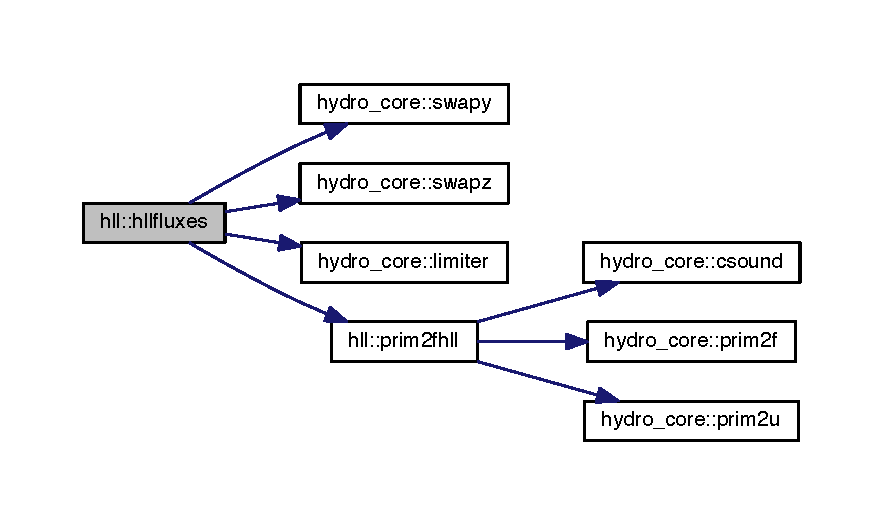
\includegraphics[width=350pt]{namespacehll_a27386fb5bcf705be5e8c2650484966c6_cgraph}
\end{center}
\end{figure}


\hypertarget{namespacehll_aa67c7db7e17f7dedf7286320baeda1dd}{}\index{hll@{hll}!prim2fhll@{prim2fhll}}
\index{prim2fhll@{prim2fhll}!hll@{hll}}
\subsubsection[{prim2fhll}]{\setlength{\rightskip}{0pt plus 5cm}subroutine hll\+::prim2fhll (
\begin{DoxyParamCaption}
\item[{real, dimension(neq), intent(in)}]{priml, }
\item[{real, dimension(neq), intent(in)}]{primr, }
\item[{real, dimension(neq), intent(inout)}]{ff}
\end{DoxyParamCaption}
)}\label{namespacehll_aa67c7db7e17f7dedf7286320baeda1dd}
Solves the Riemann problem at the interface betweem P\+L and P\+R using the H\+L\+L solver ~\newline
 The fluxes are computed in the X direction, to obtain the y ans z directions a swap is performed 
\begin{DoxyParams}{Parameters}
{\em real} & \mbox{[}in\mbox{]} prim\+L \+: primitives at the Left state \\
\hline
{\em real} & \mbox{[}in\mbox{]} prim\+R \+: primitives at the Right state \\
\hline
{\em real} & \mbox{[}out\mbox{]} ff \+: fluxes at the interface ( $ F_{i+1/2} $) \\
\hline
\end{DoxyParams}


Definition at line 48 of file hll.\+f90.



Here is the call graph for this function\+:\nopagebreak
\begin{figure}[H]
\begin{center}
\leavevmode
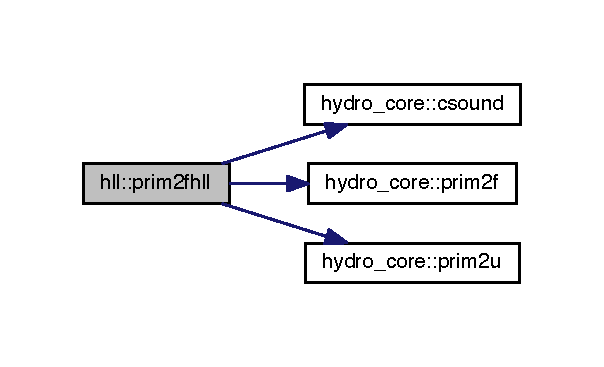
\includegraphics[width=290pt]{namespacehll_aa67c7db7e17f7dedf7286320baeda1dd_cgraph}
\end{center}
\end{figure}



\hypertarget{namespacehllc}{}\section{hllc Module Reference}
\label{namespacehllc}\index{hllc@{hllc}}


H\+L\+L\+C approximate Riemann solver module.  


\subsection*{Functions/\+Subroutines}
\begin{DoxyCompactItemize}
\item 
subroutine \hyperlink{namespacehllc_a25f1f218ed55fbda8b6311baa3ff6f80}{prim2fhllc} (priml, primr, ff)
\begin{DoxyCompactList}\small\item\em Solves the Riemann problem at the interface P\+L,P\+R using the H\+L\+L\+C solver. \end{DoxyCompactList}\item 
subroutine \hyperlink{namespacehllc_a702fd4ba2d419a6ac6d21a9bc25ba230}{hllcfluxes} (choice)
\begin{DoxyCompactList}\small\item\em Calculates H\+L\+L\+C fluxes from the primitive variables on all the domain. \end{DoxyCompactList}\end{DoxyCompactItemize}


\subsection{Detailed Description}
The module contains the routines needed to Solve the Riemann problem in the entire domain and return the physical fluxes in x,y,z with the H\+L\+L\+C solver 

\subsection{Function/\+Subroutine Documentation}
\hypertarget{namespacehllc_a702fd4ba2d419a6ac6d21a9bc25ba230}{}\index{hllc@{hllc}!hllcfluxes@{hllcfluxes}}
\index{hllcfluxes@{hllcfluxes}!hllc@{hllc}}
\subsubsection[{hllcfluxes}]{\setlength{\rightskip}{0pt plus 5cm}subroutine hllc\+::hllcfluxes (
\begin{DoxyParamCaption}
\item[{integer, intent(in)}]{choice}
\end{DoxyParamCaption}
)}\label{namespacehllc_a702fd4ba2d419a6ac6d21a9bc25ba230}
Calculates H\+L\+L\+C fluxes from the primitive variables on all the domain 
\begin{DoxyParams}{Parameters}
{\em integer} & \mbox{[}in\mbox{]} choice \+: 1, uses primit for the 1st half of timestep (first order) ~\newline
 2 uses primit for second order timestep \\
\hline
\end{DoxyParams}


Definition at line 145 of file hllc.\+f90.



Here is the call graph for this function\+:\nopagebreak
\begin{figure}[H]
\begin{center}
\leavevmode
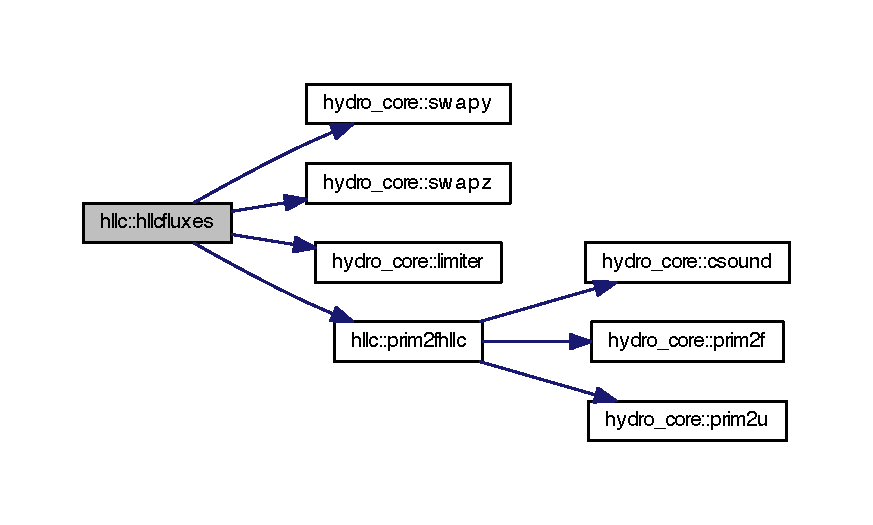
\includegraphics[width=350pt]{namespacehllc_a702fd4ba2d419a6ac6d21a9bc25ba230_cgraph}
\end{center}
\end{figure}


\hypertarget{namespacehllc_a25f1f218ed55fbda8b6311baa3ff6f80}{}\index{hllc@{hllc}!prim2fhllc@{prim2fhllc}}
\index{prim2fhllc@{prim2fhllc}!hllc@{hllc}}
\subsubsection[{prim2fhllc}]{\setlength{\rightskip}{0pt plus 5cm}subroutine hllc\+::prim2fhllc (
\begin{DoxyParamCaption}
\item[{real, dimension(neq), intent(in)}]{priml, }
\item[{real, dimension(neq), intent(in)}]{primr, }
\item[{real, dimension(neq), intent(inout)}]{ff}
\end{DoxyParamCaption}
)}\label{namespacehllc_a25f1f218ed55fbda8b6311baa3ff6f80}
Solves the Riemann problem at the interface betweem P\+L and P\+R using the H\+L\+L\+C solver ~\newline
 The fluxes are computed in the X direction, to obtain the y ans z directions a swap is performed 
\begin{DoxyParams}{Parameters}
{\em real} & \mbox{[}in\mbox{]} prim\+L \+: primitives at the Left state \\
\hline
{\em real} & \mbox{[}in\mbox{]} prim\+R \+: primitives at the Right state \\
\hline
{\em real} & \mbox{[}out\mbox{]} ff \+: fluxes at the interface ( $ F_{i+1/2} $) \\
\hline
\end{DoxyParams}


Definition at line 47 of file hllc.\+f90.



Here is the call graph for this function\+:\nopagebreak
\begin{figure}[H]
\begin{center}
\leavevmode
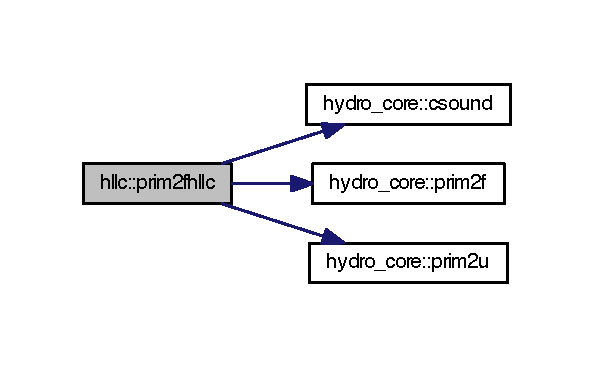
\includegraphics[width=300pt]{namespacehllc_a25f1f218ed55fbda8b6311baa3ff6f80_cgraph}
\end{center}
\end{figure}



\hypertarget{namespacehlld}{}\section{hlld Module Reference}
\label{namespacehlld}\index{hlld@{hlld}}


H\+L\+L\+D approximate Riemann solver module.  


\subsection*{Functions/\+Subroutines}
\begin{DoxyCompactItemize}
\item 
subroutine \hyperlink{namespacehlld_adb0dbc5abe3e062f2ee4e333c6794bc8}{prim2fhlld} (priml, primr, ff)
\begin{DoxyCompactList}\small\item\em Solves the Riemann problem at the interface P\+L,P\+R using the H\+L\+L\+D solver. \end{DoxyCompactList}\item 
subroutine \hyperlink{namespacehlld_a2640822e1b56d5b174f6293c26d75e22}{hlldfluxes} (choice)
\begin{DoxyCompactList}\small\item\em Calculates H\+L\+L\+D fluxes from the primitive variables on all the domain. \end{DoxyCompactList}\end{DoxyCompactItemize}


\subsection{Detailed Description}
The module contains the routines needed to Solve the Riemann problem in the entire domain and return the physical fluxes in x,y,z with the H\+L\+L\+D solver 

\subsection{Function/\+Subroutine Documentation}
\hypertarget{namespacehlld_a2640822e1b56d5b174f6293c26d75e22}{}\index{hlld@{hlld}!hlldfluxes@{hlldfluxes}}
\index{hlldfluxes@{hlldfluxes}!hlld@{hlld}}
\subsubsection[{hlldfluxes}]{\setlength{\rightskip}{0pt plus 5cm}subroutine hlld\+::hlldfluxes (
\begin{DoxyParamCaption}
\item[{integer, intent(in)}]{choice}
\end{DoxyParamCaption}
)}\label{namespacehlld_a2640822e1b56d5b174f6293c26d75e22}
Calculates H\+L\+L\+D fluxes from the primitive variables on all the domain 
\begin{DoxyParams}{Parameters}
{\em integer} & \mbox{[}in\mbox{]} choice \+: 1, uses primit for the 1st half of timestep (first order) ~\newline
 2 uses primit for second order timestep \\
\hline
\end{DoxyParams}


Definition at line 319 of file hlld.\+f90.



Here is the call graph for this function\+:\nopagebreak
\begin{figure}[H]
\begin{center}
\leavevmode
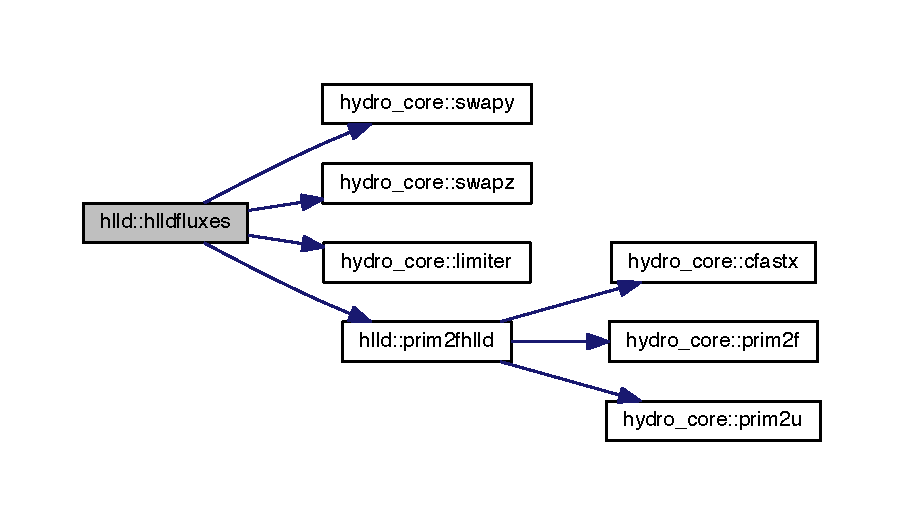
\includegraphics[width=350pt]{namespacehlld_a2640822e1b56d5b174f6293c26d75e22_cgraph}
\end{center}
\end{figure}


\hypertarget{namespacehlld_adb0dbc5abe3e062f2ee4e333c6794bc8}{}\index{hlld@{hlld}!prim2fhlld@{prim2fhlld}}
\index{prim2fhlld@{prim2fhlld}!hlld@{hlld}}
\subsubsection[{prim2fhlld}]{\setlength{\rightskip}{0pt plus 5cm}subroutine hlld\+::prim2fhlld (
\begin{DoxyParamCaption}
\item[{real, dimension(neq), intent(in)}]{priml, }
\item[{real, dimension(neq), intent(in)}]{primr, }
\item[{real, dimension(neq), intent(inout)}]{ff}
\end{DoxyParamCaption}
)}\label{namespacehlld_adb0dbc5abe3e062f2ee4e333c6794bc8}
Solves the Riemann problem at the interface betweem P\+L and P\+R using the H\+L\+L\+D solver ~\newline
 The fluxes are computed in the X direction, to obtain the y ans z directions a swap is performed 
\begin{DoxyParams}{Parameters}
{\em real} & \mbox{[}in\mbox{]} prim\+L \+: primitives at the Left state \\
\hline
{\em real} & \mbox{[}in\mbox{]} prim\+R \+: primitives at the Right state \\
\hline
{\em real} & \mbox{[}out\mbox{]} ff \+: fluxes at the interface ( $ F_{i+1/2} $) \\
\hline
\end{DoxyParams}


Definition at line 49 of file hlld.\+f90.



Here is the call graph for this function\+:\nopagebreak
\begin{figure}[H]
\begin{center}
\leavevmode
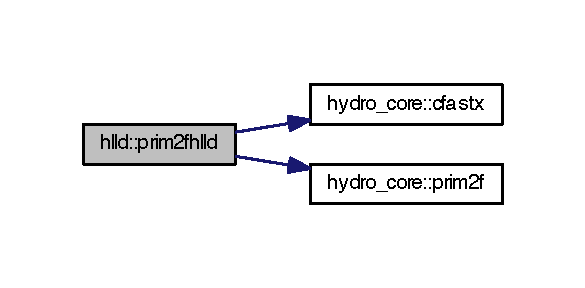
\includegraphics[width=300pt]{namespacehlld_adb0dbc5abe3e062f2ee4e333c6794bc8_cgraph}
\end{center}
\end{figure}



\hypertarget{namespacehlle}{}\section{hlle Module Reference}
\label{namespacehlle}\index{hlle@{hlle}}


H\+L\+L\+E approximate Riemann solver module.  


\subsection*{Functions/\+Subroutines}
\begin{DoxyCompactItemize}
\item 
subroutine \hyperlink{namespacehlle_a5646b0259c574b5e8dd3754a493d358d}{prim2fhlle} (priml, primr, ff)
\begin{DoxyCompactList}\small\item\em Solves the Riemann problem at the interface P\+L,P\+R using the H\+L\+L\+E solver. \end{DoxyCompactList}\item 
subroutine \hyperlink{namespacehlle_a03540214994c25ce07877114dd37b641}{hllefluxes} (choice)
\begin{DoxyCompactList}\small\item\em Calculates H\+L\+L\+E fluxes from the primitive variables on all the domain. \end{DoxyCompactList}\end{DoxyCompactItemize}


\subsection{Detailed Description}
The module contains the routines needed to Solve the Riemann problem in the entire domain and return the physical fluxes in x,y,z with the H\+L\+L\+E solver 

\subsection{Function/\+Subroutine Documentation}
\hypertarget{namespacehlle_a03540214994c25ce07877114dd37b641}{}\index{hlle@{hlle}!hllefluxes@{hllefluxes}}
\index{hllefluxes@{hllefluxes}!hlle@{hlle}}
\subsubsection[{hllefluxes}]{\setlength{\rightskip}{0pt plus 5cm}subroutine hlle\+::hllefluxes (
\begin{DoxyParamCaption}
\item[{integer, intent(in)}]{choice}
\end{DoxyParamCaption}
)}\label{namespacehlle_a03540214994c25ce07877114dd37b641}
Calculates H\+L\+L\+E fluxes from the primitive variables on all the domain 
\begin{DoxyParams}{Parameters}
{\em integer} & \mbox{[}in\mbox{]} choice \+: 1, uses primit for the 1st half of timestep (first order) ~\newline
 2 uses primit for second order timestep \\
\hline
\end{DoxyParams}


Definition at line 96 of file hlle.\+f90.



Here is the call graph for this function\+:\nopagebreak
\begin{figure}[H]
\begin{center}
\leavevmode
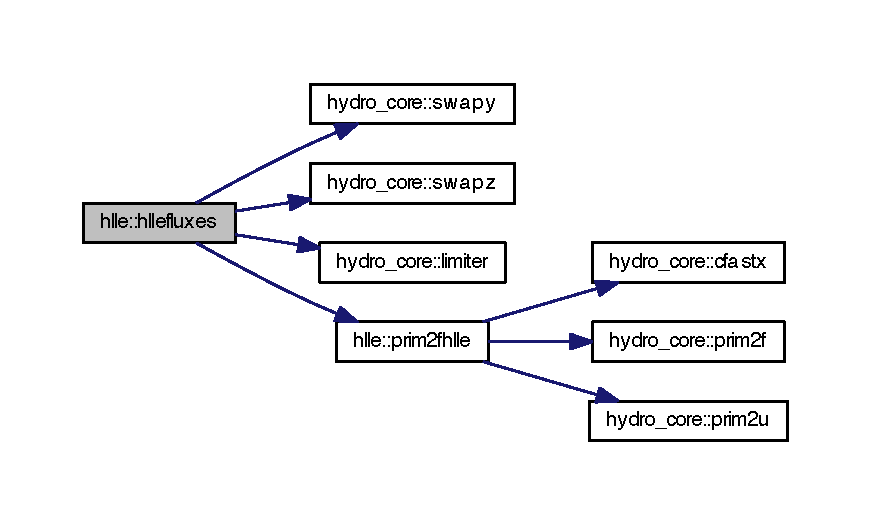
\includegraphics[width=350pt]{namespacehlle_a03540214994c25ce07877114dd37b641_cgraph}
\end{center}
\end{figure}


\hypertarget{namespacehlle_a5646b0259c574b5e8dd3754a493d358d}{}\index{hlle@{hlle}!prim2fhlle@{prim2fhlle}}
\index{prim2fhlle@{prim2fhlle}!hlle@{hlle}}
\subsubsection[{prim2fhlle}]{\setlength{\rightskip}{0pt plus 5cm}subroutine hlle\+::prim2fhlle (
\begin{DoxyParamCaption}
\item[{real, dimension(neq), intent(in)}]{priml, }
\item[{real, dimension(neq), intent(in)}]{primr, }
\item[{real, dimension(neq), intent(inout)}]{ff}
\end{DoxyParamCaption}
)}\label{namespacehlle_a5646b0259c574b5e8dd3754a493d358d}
Solves the Riemann problem at the interface betweem P\+L and P\+R using the H\+L\+L\+E solver ~\newline
 The fluxes are computed in the X direction, to obtain the y ans z directions a swap is performed 
\begin{DoxyParams}{Parameters}
{\em real} & \mbox{[}in\mbox{]} prim\+L \+: primitives at the Left state \\
\hline
{\em real} & \mbox{[}in\mbox{]} prim\+R \+: primitives at the Right state \\
\hline
{\em real} & \mbox{[}out\mbox{]} ff \+: fluxes at the interface ( $ F_{i+1/2} $) \\
\hline
\end{DoxyParams}


Definition at line 51 of file hlle.\+f90.



Here is the call graph for this function\+:\nopagebreak
\begin{figure}[H]
\begin{center}
\leavevmode
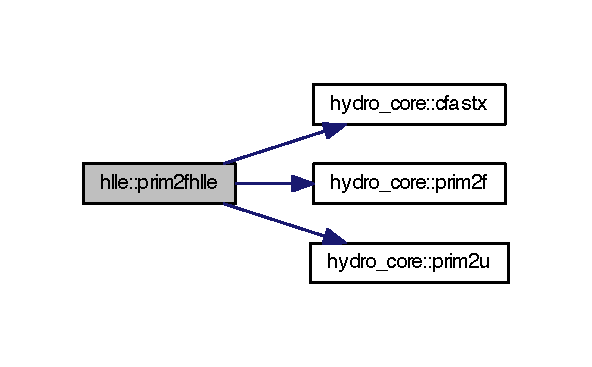
\includegraphics[width=300pt]{namespacehlle_a5646b0259c574b5e8dd3754a493d358d_cgraph}
\end{center}
\end{figure}



\hypertarget{namespacehydro__core}{}\section{hydro\+\_\+core Module Reference}
\label{namespacehydro__core}\index{hydro\+\_\+core@{hydro\+\_\+core}}


Basic hydro (and M\+H\+D) subroutines utilities.  


\subsection*{Functions/\+Subroutines}
\begin{DoxyCompactItemize}
\item 
subroutine \hyperlink{namespacehydro__core_a360e3d64343b30d94d270cfebc5b4eb3}{u2prim} (uu, prim, T)
\begin{DoxyCompactList}\small\item\em Computes the primitive variables and temperature from conserved variables on a single cell. \end{DoxyCompactList}\item 
subroutine \hyperlink{namespacehydro__core_a991a14316cc93864150071b30fd9c772}{calcprim} (u, primit)
\begin{DoxyCompactList}\small\item\em Updated the primitives, using the conserved variables in the entire domain. \end{DoxyCompactList}\item 
subroutine \hyperlink{namespacehydro__core_a98cafc8f97d7a1b3f8050b8e442194c3}{prim2u} (prim, uu)
\begin{DoxyCompactList}\small\item\em Computes the conserved conserved variables from the primitives in a single cell. \end{DoxyCompactList}\item 
subroutine \hyperlink{namespacehydro__core_a725c2c598f080ea420f4043dbda3f996}{prim2f} (prim, ff)
\begin{DoxyCompactList}\small\item\em Computes the Euler Fluxes in one cell. \end{DoxyCompactList}\item 
subroutine \hyperlink{namespacehydro__core_a64856096f7a7b7f65be1154d31916c2d}{swapy} (var, neq)
\begin{DoxyCompactList}\small\item\em Swaps the x and y components in a cell. \end{DoxyCompactList}\item 
subroutine \hyperlink{namespacehydro__core_ae4216bc7908e7665f0565aa8c885c821}{swapz} (var, neq)
\begin{DoxyCompactList}\small\item\em Swaps the x and z components in a cell. \end{DoxyCompactList}\item 
subroutine \hyperlink{namespacehydro__core_a27cb7ddb40cc0226e0139bd9eba42dfa}{csound} (p, d, cs)
\begin{DoxyCompactList}\small\item\em Computes the sound speed. \end{DoxyCompactList}\item 
subroutine \hyperlink{namespacehydro__core_ab2655b81626d4d95cb003112248e928a}{cfast} (p, d, bx, by, bz, cfx, cfy, cfz)
\begin{DoxyCompactList}\small\item\em Computes the fast magnetosonic speeds in the 3 coordinates. \end{DoxyCompactList}\item 
subroutine \hyperlink{namespacehydro__core_abd089f71325e32997703c1420db62aa8}{cfastx} (prim, cf\+X)
\begin{DoxyCompactList}\small\item\em Computes the fast magnetosonic speed in the x direction. \end{DoxyCompactList}\item 
subroutine \hyperlink{namespacehydro__core_a0b0402ba5c94d738eb020f79783f8d53}{get\+\_\+timestep} (dt)
\begin{DoxyCompactList}\small\item\em Otains the timestep allowed by the C\+F\+L condition in the entire. \end{DoxyCompactList}\item 
subroutine \hyperlink{namespacehydro__core_ada63ca89d1a40cfd1a62db0ddfdbda80}{limiter} (P\+L\+L, P\+L, P\+R, P\+R\+R, neq)
\begin{DoxyCompactList}\small\item\em Performs a linear reconstruction of the primitive variables. \end{DoxyCompactList}\end{DoxyCompactItemize}


\subsection{Detailed Description}
This module contains subroutines and utilities that are the core of the hydro (and M\+H\+D) that are common to most implementations and will be used for the different specific solvers 

\subsection{Function/\+Subroutine Documentation}
\hypertarget{namespacehydro__core_a991a14316cc93864150071b30fd9c772}{}\index{hydro\+\_\+core@{hydro\+\_\+core}!calcprim@{calcprim}}
\index{calcprim@{calcprim}!hydro\+\_\+core@{hydro\+\_\+core}}
\subsubsection[{calcprim}]{\setlength{\rightskip}{0pt plus 5cm}subroutine hydro\+\_\+core\+::calcprim (
\begin{DoxyParamCaption}
\item[{real, dimension(neq,nxmin\+:nxmax,nymin\+:nymax,nzmin\+:nzmax), intent(in)}]{u, }
\item[{real, dimension(neq,nxmin\+:nxmax,nymin\+:nymax,nzmin\+:nzmax), intent(out)}]{primit}
\end{DoxyParamCaption}
)}\label{namespacehydro__core_a991a14316cc93864150071b30fd9c772}
Updated the primitives, using the conserved variables in the entire domain 
\begin{DoxyParams}{Parameters}
{\em real} & \mbox{[}in\mbox{]} u(neq,nxmin\+:nxmax,nymin\+:nymax,nzmin\+:nzmax) \+: conserved variables \\
\hline
{\em real} & \mbox{[}out\mbox{]} prim(neq,nxmin\+:nxmax,nymin\+:nymax,nzmin\+:nzmax) \+: primitive variables \\
\hline
\end{DoxyParams}


Definition at line 116 of file hydro\+\_\+core.\+f90.



Here is the call graph for this function\+:\nopagebreak
\begin{figure}[H]
\begin{center}
\leavevmode
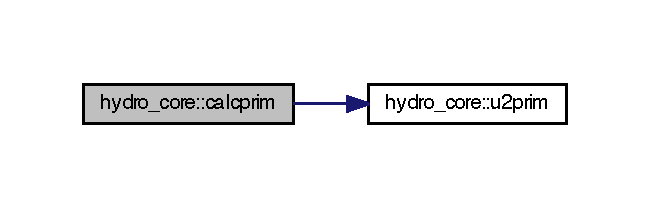
\includegraphics[width=328pt]{namespacehydro__core_a991a14316cc93864150071b30fd9c772_cgraph}
\end{center}
\end{figure}


\hypertarget{namespacehydro__core_ab2655b81626d4d95cb003112248e928a}{}\index{hydro\+\_\+core@{hydro\+\_\+core}!cfast@{cfast}}
\index{cfast@{cfast}!hydro\+\_\+core@{hydro\+\_\+core}}
\subsubsection[{cfast}]{\setlength{\rightskip}{0pt plus 5cm}subroutine hydro\+\_\+core\+::cfast (
\begin{DoxyParamCaption}
\item[{real, intent(in)}]{p, }
\item[{real, intent(in)}]{d, }
\item[{real, intent(in)}]{bx, }
\item[{real, intent(in)}]{by, }
\item[{real, intent(in)}]{bz, }
\item[{real, intent(out)}]{cfx, }
\item[{real, intent(out)}]{cfy, }
\item[{real, intent(out)}]{cfz}
\end{DoxyParamCaption}
)}\label{namespacehydro__core_ab2655b81626d4d95cb003112248e928a}
Computes the fast magnetosonic speeds in the 3 coordinates 
\begin{DoxyParams}{Parameters}
{\em real} & \mbox{[}in\mbox{]} p \+: value of pressure \\
\hline
{\em real} & \mbox{[}in\mbox{]} d \+: value of density \\
\hline
{\em real} & \mbox{[}in\mbox{]} Bx \+: value of the x component of the magnetic field \\
\hline
{\em real} & \mbox{[}in\mbox{]} By \+: value of the y component of the magnetic field \\
\hline
{\em real} & \mbox{[}in\mbox{]} Bz \+: value of the z component of the magnetic field \\
\hline
{\em real} & \mbox{[}out\mbox{]} csx \+: fast magnetisonic speed in x \\
\hline
{\em real} & \mbox{[}out\mbox{]} csy \+: fast magnetisonic speed in y \\
\hline
{\em real} & \mbox{[}out\mbox{]} csz \+: fast magnetisonic speed in z \\
\hline
\end{DoxyParams}


Definition at line 325 of file hydro\+\_\+core.\+f90.

\hypertarget{namespacehydro__core_abd089f71325e32997703c1420db62aa8}{}\index{hydro\+\_\+core@{hydro\+\_\+core}!cfastx@{cfastx}}
\index{cfastx@{cfastx}!hydro\+\_\+core@{hydro\+\_\+core}}
\subsubsection[{cfastx}]{\setlength{\rightskip}{0pt plus 5cm}subroutine hydro\+\_\+core\+::cfastx (
\begin{DoxyParamCaption}
\item[{real, dimension(neq), intent(in)}]{prim, }
\item[{real, intent(out)}]{cf\+X}
\end{DoxyParamCaption}
)}\label{namespacehydro__core_abd089f71325e32997703c1420db62aa8}
Computes the fast magnetosonic speed in the x direction 
\begin{DoxyParams}{Parameters}
{\em real} & \mbox{[}in\mbox{]} prim(neq) \+: vector with the primitives in one cell \\
\hline
\end{DoxyParams}


Definition at line 350 of file hydro\+\_\+core.\+f90.

\hypertarget{namespacehydro__core_a27cb7ddb40cc0226e0139bd9eba42dfa}{}\index{hydro\+\_\+core@{hydro\+\_\+core}!csound@{csound}}
\index{csound@{csound}!hydro\+\_\+core@{hydro\+\_\+core}}
\subsubsection[{csound}]{\setlength{\rightskip}{0pt plus 5cm}subroutine hydro\+\_\+core\+::csound (
\begin{DoxyParamCaption}
\item[{real, intent(in)}]{p, }
\item[{real, intent(in)}]{d, }
\item[{real, intent(out)}]{cs}
\end{DoxyParamCaption}
)}\label{namespacehydro__core_a27cb7ddb40cc0226e0139bd9eba42dfa}
Computes the sound speed 
\begin{DoxyParams}{Parameters}
{\em real} & \mbox{[}in\mbox{]} p \+: value of pressure \\
\hline
{\em real} & \mbox{[}in\mbox{]} d \+: value of density \\
\hline
{\em real} & \mbox{[}out\mbox{]} cs \+: sound speed \\
\hline
\end{DoxyParams}


Definition at line 299 of file hydro\+\_\+core.\+f90.

\hypertarget{namespacehydro__core_a0b0402ba5c94d738eb020f79783f8d53}{}\index{hydro\+\_\+core@{hydro\+\_\+core}!get\+\_\+timestep@{get\+\_\+timestep}}
\index{get\+\_\+timestep@{get\+\_\+timestep}!hydro\+\_\+core@{hydro\+\_\+core}}
\subsubsection[{get\+\_\+timestep}]{\setlength{\rightskip}{0pt plus 5cm}subroutine hydro\+\_\+core\+::get\+\_\+timestep (
\begin{DoxyParamCaption}
\item[{real, intent(out)}]{dt}
\end{DoxyParamCaption}
)}\label{namespacehydro__core_a0b0402ba5c94d738eb020f79783f8d53}
Otains the timestep allowed by the C\+F\+L condition in the entire domain using the global primitives 
\begin{DoxyParams}{Parameters}
{\em real} & \mbox{[}out\mbox{]} \+: $ \Delta t$ allowed by the C\+F\+L condition \\
\hline
\end{DoxyParams}


Definition at line 373 of file hydro\+\_\+core.\+f90.



Here is the call graph for this function\+:\nopagebreak
\begin{figure}[H]
\begin{center}
\leavevmode
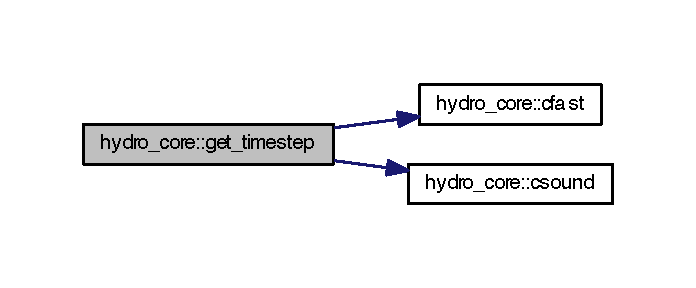
\includegraphics[width=349pt]{namespacehydro__core_a0b0402ba5c94d738eb020f79783f8d53_cgraph}
\end{center}
\end{figure}


\hypertarget{namespacehydro__core_ada63ca89d1a40cfd1a62db0ddfdbda80}{}\index{hydro\+\_\+core@{hydro\+\_\+core}!limiter@{limiter}}
\index{limiter@{limiter}!hydro\+\_\+core@{hydro\+\_\+core}}
\subsubsection[{limiter}]{\setlength{\rightskip}{0pt plus 5cm}subroutine hydro\+\_\+core\+::limiter (
\begin{DoxyParamCaption}
\item[{real, dimension(neq), intent(in)}]{P\+L\+L, }
\item[{real, dimension(neq), intent(inout)}]{P\+L, }
\item[{real, dimension(neq), intent(inout)}]{P\+R, }
\item[{real, dimension(neq), intent(in)}]{P\+R\+R, }
\item[{integer, intent(in)}]{neq}
\end{DoxyParamCaption}
)}\label{namespacehydro__core_ada63ca89d1a40cfd1a62db0ddfdbda80}
returns a linear reconstruction of the variables at the interface beteen the primitives P\+L\+L, P\+L, P\+R, P\+R\+R ~\newline
 The reconstruction is made with a slope limiter chosen at compilation time (i.\+e. set on the Makefile) 
\begin{DoxyParams}{Parameters}
{\em real} & \mbox{[}in\mbox{]} \+: primitives at the left of the left state \\
\hline
{\em real} & \mbox{[}inout\mbox{]} \+: primitives at the left state \\
\hline
{\em real} & \mbox{[}inout\mbox{]} \+: primitives at the right state \\
\hline
{\em real} & \mbox{[}in\mbox{]} \+: primitives at the right of the right state \\
\hline
{\em real} & \mbox{[}in\mbox{]} \+: number of equations \\
\hline
\end{DoxyParams}


Definition at line 437 of file hydro\+\_\+core.\+f90.

\hypertarget{namespacehydro__core_a725c2c598f080ea420f4043dbda3f996}{}\index{hydro\+\_\+core@{hydro\+\_\+core}!prim2f@{prim2f}}
\index{prim2f@{prim2f}!hydro\+\_\+core@{hydro\+\_\+core}}
\subsubsection[{prim2f}]{\setlength{\rightskip}{0pt plus 5cm}subroutine hydro\+\_\+core\+::prim2f (
\begin{DoxyParamCaption}
\item[{real, dimension(neq), intent(in)}]{prim, }
\item[{real, dimension(neq), intent(out)}]{ff}
\end{DoxyParamCaption}
)}\label{namespacehydro__core_a725c2c598f080ea420f4043dbda3f996}
Computes the Euler Fluxes in one cell, using the primitices ~\newline
 It returns the flux in the x direction (i.\+e. F), the y and z fluxes can be obtained swaping the respective entries (see swapy and swapz subroutines) 
\begin{DoxyParams}{Parameters}
{\em real} & \mbox{[}in\mbox{]} prim(neq) \+: primitives in one cell \\
\hline
{\em real} & \mbox{[}out\mbox{]} ff(neq) \+: Euler Fluxes (x direction) \\
\hline
\end{DoxyParams}


Definition at line 196 of file hydro\+\_\+core.\+f90.

\hypertarget{namespacehydro__core_a98cafc8f97d7a1b3f8050b8e442194c3}{}\index{hydro\+\_\+core@{hydro\+\_\+core}!prim2u@{prim2u}}
\index{prim2u@{prim2u}!hydro\+\_\+core@{hydro\+\_\+core}}
\subsubsection[{prim2u}]{\setlength{\rightskip}{0pt plus 5cm}subroutine hydro\+\_\+core\+::prim2u (
\begin{DoxyParamCaption}
\item[{real, dimension(neq), intent(in)}]{prim, }
\item[{real, dimension(neq), intent(out)}]{uu}
\end{DoxyParamCaption}
)}\label{namespacehydro__core_a98cafc8f97d7a1b3f8050b8e442194c3}
Computes the conserved conserved variables from the primitives in a single cell 
\begin{DoxyParams}{Parameters}
{\em real} & \mbox{[}in\mbox{]} prim(neq) \+: primitives in one cell \\
\hline
{\em real} & \mbox{[}out\mbox{]} uu(neq) \+: conserved varibles in one cell \\
\hline
\end{DoxyParams}


Definition at line 155 of file hydro\+\_\+core.\+f90.

\hypertarget{namespacehydro__core_a64856096f7a7b7f65be1154d31916c2d}{}\index{hydro\+\_\+core@{hydro\+\_\+core}!swapy@{swapy}}
\index{swapy@{swapy}!hydro\+\_\+core@{hydro\+\_\+core}}
\subsubsection[{swapy}]{\setlength{\rightskip}{0pt plus 5cm}subroutine hydro\+\_\+core\+::swapy (
\begin{DoxyParamCaption}
\item[{real, dimension(neq), intent(inout)}]{var, }
\item[{integer, intent(in)}]{neq}
\end{DoxyParamCaption}
)}\label{namespacehydro__core_a64856096f7a7b7f65be1154d31916c2d}
Swaps the x and y components in a cell. 
\begin{DoxyParams}{Parameters}
{\em real} & \mbox{[}inout\mbox{]} var(neq) \+: variable to be swapped \\
\hline
{\em real} & \mbox{[}in\mbox{]} neq \+: number of equations in the code \\
\hline
\end{DoxyParams}


Definition at line 247 of file hydro\+\_\+core.\+f90.

\hypertarget{namespacehydro__core_ae4216bc7908e7665f0565aa8c885c821}{}\index{hydro\+\_\+core@{hydro\+\_\+core}!swapz@{swapz}}
\index{swapz@{swapz}!hydro\+\_\+core@{hydro\+\_\+core}}
\subsubsection[{swapz}]{\setlength{\rightskip}{0pt plus 5cm}subroutine hydro\+\_\+core\+::swapz (
\begin{DoxyParamCaption}
\item[{real, dimension(neq), intent(inout)}]{var, }
\item[{integer, intent(in)}]{neq}
\end{DoxyParamCaption}
)}\label{namespacehydro__core_ae4216bc7908e7665f0565aa8c885c821}
Swaps the x and z components in a cell. 
\begin{DoxyParams}{Parameters}
{\em real} & \mbox{[}inout\mbox{]} var(neq) \+: variable to be swapped \\
\hline
{\em real} & \mbox{[}in\mbox{]} neq \+: number of equations in the code \\
\hline
\end{DoxyParams}


Definition at line 273 of file hydro\+\_\+core.\+f90.

\hypertarget{namespacehydro__core_a360e3d64343b30d94d270cfebc5b4eb3}{}\index{hydro\+\_\+core@{hydro\+\_\+core}!u2prim@{u2prim}}
\index{u2prim@{u2prim}!hydro\+\_\+core@{hydro\+\_\+core}}
\subsubsection[{u2prim}]{\setlength{\rightskip}{0pt plus 5cm}subroutine hydro\+\_\+core\+::u2prim (
\begin{DoxyParamCaption}
\item[{real, dimension(neq), intent(in)}]{uu, }
\item[{real, dimension(neq), intent(out)}]{prim, }
\item[{real, intent(out)}]{T}
\end{DoxyParamCaption}
)}\label{namespacehydro__core_a360e3d64343b30d94d270cfebc5b4eb3}
Computes the primitive variables and temperature from conserved variables on a single cell 
\begin{DoxyParams}{Parameters}
{\em real} & \mbox{[}in\mbox{]} uu(neq) \+: conserved variables in one cell \\
\hline
{\em real} & \mbox{[}out\mbox{]} prim(neq) \+: primitives in one cell \\
\hline
{\em real} & \mbox{[}out\mbox{]} T \+: Temperature \mbox{[}K\mbox{]} \\
\hline
\end{DoxyParams}


Definition at line 44 of file hydro\+\_\+core.\+f90.


\hypertarget{namespacehydro__solver}{}\section{hydro\+\_\+solver Module Reference}
\label{namespacehydro__solver}\index{hydro\+\_\+solver@{hydro\+\_\+solver}}


Advances the simulation one timestep.  


\subsection*{Functions/\+Subroutines}
\begin{DoxyCompactItemize}
\item 
subroutine \hyperlink{namespacehydro__solver_a88127baf969063d6d9a31845fa7c1835}{viscosity} ()
\begin{DoxyCompactList}\small\item\em Adds artificial viscosity to the conserved variables. \end{DoxyCompactList}\item 
subroutine \hyperlink{namespacehydro__solver_ac34a166e9ddd81f20f2b271138458a1a}{step} (dt)
\begin{DoxyCompactList}\small\item\em Upwind timestep. \end{DoxyCompactList}\item 
subroutine \hyperlink{namespacehydro__solver_aa95013d45fe4922819805e68527ab3b5}{tstep} ()
\begin{DoxyCompactList}\small\item\em High level wrapper to advancce the simulation. \end{DoxyCompactList}\end{DoxyCompactItemize}


\subsection{Detailed Description}
Advances the solution from $ t $ to $ t + \Delta t $ 

\subsection{Function/\+Subroutine Documentation}
\hypertarget{namespacehydro__solver_ac34a166e9ddd81f20f2b271138458a1a}{}\index{hydro\+\_\+solver@{hydro\+\_\+solver}!step@{step}}
\index{step@{step}!hydro\+\_\+solver@{hydro\+\_\+solver}}
\subsubsection[{step}]{\setlength{\rightskip}{0pt plus 5cm}subroutine hydro\+\_\+solver\+::step (
\begin{DoxyParamCaption}
\item[{real, intent(in)}]{dt}
\end{DoxyParamCaption}
)}\label{namespacehydro__solver_ac34a166e9ddd81f20f2b271138458a1a}
Performs the upwind timestep according to \[ U^{n+1}_i= U^n_i -\frac{\Delta t}{\Delta x} \left[F^{n+1/2}_{i+1/2}-F^{n+1/2}_{i-1/2} \right] \] (in 3\+D), it takes $ U^{n+1} $=up from the global variables and $ U^{n} $=u 
\begin{DoxyParams}{Parameters}
{\em real} & \mbox{[}in\mbox{]} dt \+: timestep \\
\hline
\end{DoxyParams}


Definition at line 84 of file hydro\+\_\+solver.\+f90.



Here is the call graph for this function\+:
% FIG 0


\hypertarget{namespacehydro__solver_aa95013d45fe4922819805e68527ab3b5}{}\index{hydro\+\_\+solver@{hydro\+\_\+solver}!tstep@{tstep}}
\index{tstep@{tstep}!hydro\+\_\+solver@{hydro\+\_\+solver}}
\subsubsection[{tstep}]{\setlength{\rightskip}{0pt plus 5cm}subroutine hydro\+\_\+solver\+::tstep (
\begin{DoxyParamCaption}
{}
\end{DoxyParamCaption}
)}\label{namespacehydro__solver_aa95013d45fe4922819805e68527ab3b5}
High level wrapper to advancce the simulation ~\newline
 The variables are taken from the globals module. 

Definition at line 126 of file hydro\+\_\+solver.\+f90.



Here is the call graph for this function\+:
% FIG 1


\hypertarget{namespacehydro__solver_a88127baf969063d6d9a31845fa7c1835}{}\index{hydro\+\_\+solver@{hydro\+\_\+solver}!viscosity@{viscosity}}
\index{viscosity@{viscosity}!hydro\+\_\+solver@{hydro\+\_\+solver}}
\subsubsection[{viscosity}]{\setlength{\rightskip}{0pt plus 5cm}subroutine hydro\+\_\+solver\+::viscosity (
\begin{DoxyParamCaption}
{}
\end{DoxyParamCaption}
)}\label{namespacehydro__solver_a88127baf969063d6d9a31845fa7c1835}
Adds artificial viscosity to the conserved variables ~\newline
 Takes the variables from the globals module and it assumes that the up are the stepped variables, while u are unstepped 

Definition at line 54 of file hydro\+\_\+solver.\+f90.


\hypertarget{namespaceinit}{}\section{init Module Reference}
\label{namespaceinit}\index{init@{init}}


Guacho-\/3\+D initialization.  


\subsection*{Functions/\+Subroutines}
\begin{DoxyCompactItemize}
\item 
subroutine \hyperlink{namespaceinit_a60b4d8ee577d59490c7d351b73253a99}{initmain} (tprint, itprint)
\begin{DoxyCompactList}\small\item\em Main initialization routine. \end{DoxyCompactList}\item 
subroutine \hyperlink{namespaceinit_ab5415b25da1a9e732d3f557f4d6008b9}{initflow} (itprint)
\begin{DoxyCompactList}\small\item\em Initializes the conserved variables, in the globals module. \end{DoxyCompactList}\end{DoxyCompactItemize}


\subsection{Detailed Description}
This module contains the routines needed to initializa the code, it also initiaizes all the modules set by the user. 

\subsection{Function/\+Subroutine Documentation}
\hypertarget{namespaceinit_ab5415b25da1a9e732d3f557f4d6008b9}{}\index{init@{init}!initflow@{initflow}}
\index{initflow@{initflow}!init@{init}}
\subsubsection[{initflow}]{\setlength{\rightskip}{0pt plus 5cm}subroutine init\+::initflow (
\begin{DoxyParamCaption}
\item[{integer, intent(inout)}]{itprint}
\end{DoxyParamCaption}
)}\label{namespaceinit_ab5415b25da1a9e732d3f557f4d6008b9}
Initializes the conserved variables, in the globals module 
\begin{DoxyParams}{Parameters}
{\em real} & \mbox{[}inout\mbox{]} itprint \+: number of current output \\
\hline
\end{DoxyParams}


Definition at line 435 of file init.\+f90.

\hypertarget{namespaceinit_a60b4d8ee577d59490c7d351b73253a99}{}\index{init@{init}!initmain@{initmain}}
\index{initmain@{initmain}!init@{init}}
\subsubsection[{initmain}]{\setlength{\rightskip}{0pt plus 5cm}subroutine init\+::initmain (
\begin{DoxyParamCaption}
\item[{real, intent(out)}]{tprint, }
\item[{integer, intent(out)}]{itprint}
\end{DoxyParamCaption}
)}\label{namespaceinit_a60b4d8ee577d59490c7d351b73253a99}
This subsroutine initializes all the variables in the globals module, M\+P\+I, cooling and user\+\_\+mod routines; and outputs to screen the main parameters used in the run 
\begin{DoxyParams}{Parameters}
{\em real} & \mbox{[}out\mbox{]} tprint \+: time of next output \\
\hline
{\em integer} & \mbox{[}out\mbox{]} itprint \+: number of next output \\
\hline
\end{DoxyParams}


Definition at line 41 of file init.\+f90.



Here is the call graph for this function\+:
% FIG 0



\hypertarget{namespacelinear__system}{}\section{linear\+\_\+system Module Reference}
\label{namespacelinear__system}\index{linear\+\_\+system@{linear\+\_\+system}}


linear system inversion module  


\subsection*{Functions/\+Subroutines}
\begin{DoxyCompactItemize}
\item 
subroutine \hyperlink{namespacelinear__system_ad77fb788295266bcc818f72d6677bf9d}{ludcmp} (a, n, indx, d)
\begin{DoxyCompactList}\small\item\em L\+U decomposition. \end{DoxyCompactList}\item 
subroutine \hyperlink{namespacelinear__system_acdd63cedefa6077e4100904703d6b82d}{lubksb} (a, n, indx, b)
\begin{DoxyCompactList}\small\item\em Solves a set of linear equations. \end{DoxyCompactList}\item 
subroutine \hyperlink{namespacelinear__system_a51e9428c30e00182fa86755204de7762}{linsys} (a, b, n)
\begin{DoxyCompactList}\small\item\em Driver to solves a set of linear equations. \end{DoxyCompactList}\end{DoxyCompactItemize}


\subsection{Detailed Description}
Inversion of a system of linear equations with an L\+U decomposition method (these routines are from Numerical Methods by Press et al.) 

\subsection{Function/\+Subroutine Documentation}
\hypertarget{namespacelinear__system_a51e9428c30e00182fa86755204de7762}{}\index{linear\+\_\+system@{linear\+\_\+system}!linsys@{linsys}}
\index{linsys@{linsys}!linear\+\_\+system@{linear\+\_\+system}}
\subsubsection[{linsys}]{\setlength{\rightskip}{0pt plus 5cm}subroutine linear\+\_\+system\+::linsys (
\begin{DoxyParamCaption}
\item[{real (kind=8), dimension(n,n)}]{a, }
\item[{real (kind=8), dimension(n)}]{b, }
\item[{integer, intent(in)}]{n}
\end{DoxyParamCaption}
)}\label{namespacelinear__system_a51e9428c30e00182fa86755204de7762}
Solves a linear set of equations 

Definition at line 178 of file linear\+\_\+system.\+f90.



Here is the call graph for this function\+:
% FIG 0


\hypertarget{namespacelinear__system_acdd63cedefa6077e4100904703d6b82d}{}\index{linear\+\_\+system@{linear\+\_\+system}!lubksb@{lubksb}}
\index{lubksb@{lubksb}!linear\+\_\+system@{linear\+\_\+system}}
\subsubsection[{lubksb}]{\setlength{\rightskip}{0pt plus 5cm}subroutine linear\+\_\+system\+::lubksb (
\begin{DoxyParamCaption}
\item[{real (kind=8), dimension(n,n), intent(in)}]{a, }
\item[{integer, intent(in)}]{n, }
\item[{integer, dimension(n), intent(in)}]{indx, }
\item[{real (kind=8), dimension(n), intent(inout)}]{b}
\end{DoxyParamCaption}
)}\label{namespacelinear__system_acdd63cedefa6077e4100904703d6b82d}
Solves a linear set of equations of the form 

Definition at line 129 of file linear\+\_\+system.\+f90.

\hypertarget{namespacelinear__system_ad77fb788295266bcc818f72d6677bf9d}{}\index{linear\+\_\+system@{linear\+\_\+system}!ludcmp@{ludcmp}}
\index{ludcmp@{ludcmp}!linear\+\_\+system@{linear\+\_\+system}}
\subsubsection[{ludcmp}]{\setlength{\rightskip}{0pt plus 5cm}subroutine linear\+\_\+system\+::ludcmp (
\begin{DoxyParamCaption}
\item[{real (kind=8), dimension(n,n), intent(inout)}]{a, }
\item[{integer, intent(in)}]{n, }
\item[{integer, dimension(n), intent(out)}]{indx, }
\item[{real (kind=8), intent(inout)}]{d}
\end{DoxyParamCaption}
)}\label{namespacelinear__system_ad77fb788295266bcc818f72d6677bf9d}
L\+U decomposition of a row-\/wise permutation 
\begin{DoxyParams}{Parameters}
{\em real} & \mbox{[}inout\mbox{]} a(n,n) \+: matrix to be decomposed result is done in place \\
\hline
{\em integer} & \mbox{[}in\mbox{]} n \+: size of the matrix \\
\hline
{\em real} & \mbox{[}out\mbox{]} index(n) \+: vector that contains the row permutation affected by the partial pivoting \\
\hline
{\em integer} & \mbox{[}inout\mbox{]} d \+: +/-\/ 1 depending if the row intergarches is even or odd \\
\hline
\end{DoxyParams}


Definition at line 46 of file linear\+\_\+system.\+f90.


\hypertarget{namespacelyman__alpha__utilities}{}\section{lyman\+\_\+alpha\+\_\+utilities Module Reference}
\label{namespacelyman__alpha__utilities}\index{lyman\+\_\+alpha\+\_\+utilities@{lyman\+\_\+alpha\+\_\+utilities}}


Lyman\+\_\+alpha\+\_\+utilities.  


\subsection*{Functions/\+Subroutines}
\begin{DoxyCompactItemize}
\item 
subroutine \hyperlink{namespacelyman__alpha__utilities_a5f97eeffb7ea030271481514d7072efb}{init\+\_\+la} ()
\begin{DoxyCompactList}\small\item\em Initializes data. \end{DoxyCompactList}\item 
subroutine \hyperlink{namespacelyman__alpha__utilities_a75d86f06c6da27d0754752c23c50b54a}{read\+\_\+data} (u, itprint, filepath)
\begin{DoxyCompactList}\small\item\em reads data from file \end{DoxyCompactList}\item 
subroutine \hyperlink{namespacelyman__alpha__utilities_abdefc59ee98b1526aa3116c0e8f21d98}{getxyz} (i, j, k, x, y, z)
\begin{DoxyCompactList}\small\item\em gets position of a cell \end{DoxyCompactList}\item 
subroutine \hyperlink{namespacelyman__alpha__utilities_afaddcbb27f079d4300ce631609bbb80d}{rotation\+\_\+x} (theta, x, y, z, xn, yn, zn)
\begin{DoxyCompactList}\small\item\em Rotation around the X axis. \end{DoxyCompactList}\item 
subroutine \hyperlink{namespacelyman__alpha__utilities_ae865cec09dd956ff966316caf8ac0c9a}{rotation\+\_\+y} (theta, x, y, z, xn, yn, zn)
\begin{DoxyCompactList}\small\item\em Rotation around the Y axis. \end{DoxyCompactList}\item 
subroutine \hyperlink{namespacelyman__alpha__utilities_a2c97c4405186edcb70d2e37bbe7306da}{rotation\+\_\+z} (theta, x, y, z, xn, yn, zn)
\begin{DoxyCompactList}\small\item\em Rotation around the Z axis. \end{DoxyCompactList}\item 
subroutine \hyperlink{namespacelyman__alpha__utilities_a7ca5810d29123f1c5c6fd3170f5f5bf3}{fill\+\_\+map} (nxmap, nymap, nvmap, vmin, vmax, u, map, dx\+T, dy\+T, theta\+\_\+x, theta\+\_\+y, theta\+\_\+z)
\begin{DoxyCompactList}\small\item\em Fill target map. \end{DoxyCompactList}\item 
subroutine \hyperlink{namespacelyman__alpha__utilities_afdab7ea06bb95956c43102154651cfd1}{write\+\_\+la} (itprint, filepath, nxmap, nymap, nvmap, map)
\begin{DoxyCompactList}\small\item\em Writes projection to file. \end{DoxyCompactList}\item 
subroutine \hyperlink{namespacelyman__alpha__utilities_a826e6fe44f66513e5a47f2b968e1d0b8}{phigauss} (T, vzn, vmin, vmax, nvmap, profile)
\begin{DoxyCompactList}\small\item\em This routine computes a gaussian line profile. \end{DoxyCompactList}\end{DoxyCompactItemize}


\subsection{Detailed Description}
Utilities to compute the Lyman-\/  

\subsection{Function/\+Subroutine Documentation}
\hypertarget{namespacelyman__alpha__utilities_a7ca5810d29123f1c5c6fd3170f5f5bf3}{}\index{lyman\+\_\+alpha\+\_\+utilities@{lyman\+\_\+alpha\+\_\+utilities}!fill\+\_\+map@{fill\+\_\+map}}
\index{fill\+\_\+map@{fill\+\_\+map}!lyman\+\_\+alpha\+\_\+utilities@{lyman\+\_\+alpha\+\_\+utilities}}
\subsubsection[{fill\+\_\+map}]{\setlength{\rightskip}{0pt plus 5cm}subroutine lyman\+\_\+alpha\+\_\+utilities\+::fill\+\_\+map (
\begin{DoxyParamCaption}
\item[{integer, intent(in)}]{nxmap, }
\item[{integer, intent(in)}]{nymap, }
\item[{integer, intent(in)}]{nvmap, }
\item[{real, intent(in)}]{vmin, }
\item[{real, intent(in)}]{vmax, }
\item[{real, dimension(neq,nxmin\+:nxmax,nymin\+:nymax, nzmin\+:nzmax), intent(in)}]{u, }
\item[{real, dimension(nxmap,nymap,nvmap), intent(out)}]{map, }
\item[{real, intent(in)}]{dx\+T, }
\item[{real, intent(in)}]{dy\+T, }
\item[{real, intent(in)}]{theta\+\_\+x, }
\item[{real, intent(in)}]{theta\+\_\+y, }
\item[{real, intent(in)}]{theta\+\_\+z}
\end{DoxyParamCaption}
)}\label{namespacelyman__alpha__utilities_a7ca5810d29123f1c5c6fd3170f5f5bf3}
Fills the target map of one M\+P\+I block 
\begin{DoxyParams}{Parameters}
{\em integer} & \mbox{[}in\mbox{]} nxmap \+: Number of X cells in target \\
\hline
{\em integer} & \mbox{[}in\mbox{]} nymap \+: Number of Y cells in target \\
\hline
{\em real} & \mbox{[}in\mbox{]} u(neq,nxmin\+:nxmax,nymin\+:nymax, nzmin\+:nzmax) \+: conserved variables \\
\hline
{\em real} & \mbox{[}out\mbox{]} map(nxmap,mymap) \+: Target map \\
\hline
{\em real} & \mbox{[}in\mbox{]} dx\+T \+: target pixel width \\
\hline
{\em real} & \mbox{[}in\mbox{]} dy\+T \+: target pixel height \\
\hline
{\em real} & \mbox{[}in\mbox{]} thetax \+: Rotation around X \\
\hline
{\em real} & \mbox{[}in\mbox{]} thetay \+: Rotation around Y \\
\hline
{\em real} & \mbox{[}in\mbox{]} thetaz \+: Rotation around Z \\
\hline
\end{DoxyParams}


Definition at line 285 of file lyman\+\_\+alpha\+\_\+tau.\+f90.



Here is the call graph for this function\+:\nopagebreak
\begin{figure}[H]
\begin{center}
\leavevmode
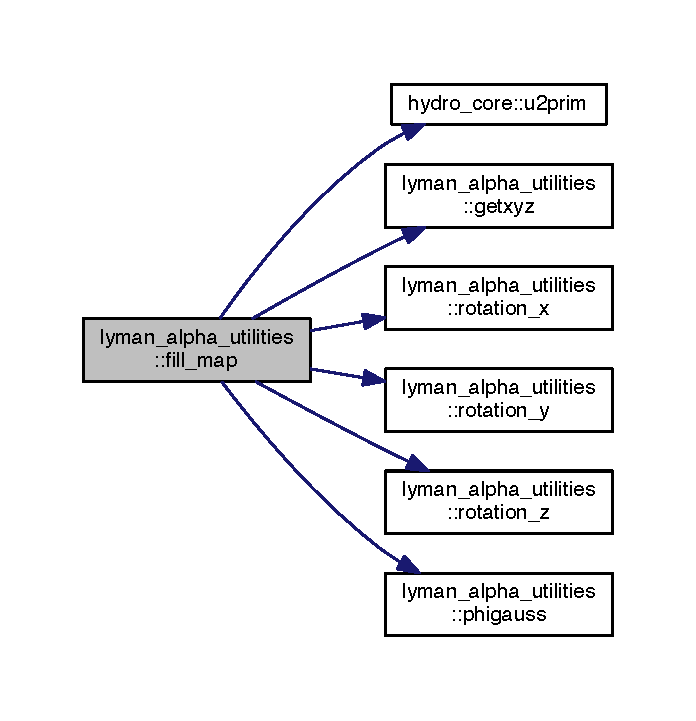
\includegraphics[width=324pt]{namespacelyman__alpha__utilities_a7ca5810d29123f1c5c6fd3170f5f5bf3_cgraph}
\end{center}
\end{figure}


\hypertarget{namespacelyman__alpha__utilities_abdefc59ee98b1526aa3116c0e8f21d98}{}\index{lyman\+\_\+alpha\+\_\+utilities@{lyman\+\_\+alpha\+\_\+utilities}!getxyz@{getxyz}}
\index{getxyz@{getxyz}!lyman\+\_\+alpha\+\_\+utilities@{lyman\+\_\+alpha\+\_\+utilities}}
\subsubsection[{getxyz}]{\setlength{\rightskip}{0pt plus 5cm}subroutine lyman\+\_\+alpha\+\_\+utilities\+::getxyz (
\begin{DoxyParamCaption}
\item[{integer, intent(in)}]{i, }
\item[{integer, intent(in)}]{j, }
\item[{integer, intent(in)}]{k, }
\item[{real, intent(out)}]{x, }
\item[{real, intent(out)}]{y, }
\item[{real, intent(out)}]{z}
\end{DoxyParamCaption}
)}\label{namespacelyman__alpha__utilities_abdefc59ee98b1526aa3116c0e8f21d98}
Returns the position and spherical radius calculated with respect to the center of the grid 
\begin{DoxyParams}{Parameters}
{\em integer} & \mbox{[}in\mbox{]} i \+: cell index in the x direction \\
\hline
{\em integer} & \mbox{[}in\mbox{]} j \+: cell index in the y direction \\
\hline
{\em integer} & \mbox{[}in\mbox{]} k \+: cell index in the z direction \\
\hline
{\em real} & \mbox{[}in\mbox{]} x \+: x position in the grid \\
\hline
{\em real} & \mbox{[}in\mbox{]} y \+: y position in the grid \\
\hline
{\em real} & \mbox{[}in\mbox{]} z \+: z position in the grid \\
\hline
\end{DoxyParams}


Definition at line 186 of file lyman\+\_\+alpha\+\_\+tau.\+f90.

\hypertarget{namespacelyman__alpha__utilities_a5f97eeffb7ea030271481514d7072efb}{}\index{lyman\+\_\+alpha\+\_\+utilities@{lyman\+\_\+alpha\+\_\+utilities}!init\+\_\+la@{init\+\_\+la}}
\index{init\+\_\+la@{init\+\_\+la}!lyman\+\_\+alpha\+\_\+utilities@{lyman\+\_\+alpha\+\_\+utilities}}
\subsubsection[{init\+\_\+la}]{\setlength{\rightskip}{0pt plus 5cm}subroutine lyman\+\_\+alpha\+\_\+utilities\+::init\+\_\+la (
\begin{DoxyParamCaption}
{}
\end{DoxyParamCaption}
)}\label{namespacelyman__alpha__utilities_a5f97eeffb7ea030271481514d7072efb}
Initializes data, M\+P\+I and other stuff 

Definition at line 36 of file lyman\+\_\+alpha\+\_\+tau.\+f90.

\hypertarget{namespacelyman__alpha__utilities_a826e6fe44f66513e5a47f2b968e1d0b8}{}\index{lyman\+\_\+alpha\+\_\+utilities@{lyman\+\_\+alpha\+\_\+utilities}!phigauss@{phigauss}}
\index{phigauss@{phigauss}!lyman\+\_\+alpha\+\_\+utilities@{lyman\+\_\+alpha\+\_\+utilities}}
\subsubsection[{phigauss}]{\setlength{\rightskip}{0pt plus 5cm}subroutine lyman\+\_\+alpha\+\_\+utilities\+::phigauss (
\begin{DoxyParamCaption}
\item[{real, intent(in)}]{T, }
\item[{real, intent(in)}]{vzn, }
\item[{real, intent(in)}]{vmin, }
\item[{real, intent(in)}]{vmax, }
\item[{integer, intent(in)}]{nvmap, }
\item[{real, dimension(nvmap), intent(out)}]{profile}
\end{DoxyParamCaption}
)}\label{namespacelyman__alpha__utilities_a826e6fe44f66513e5a47f2b968e1d0b8}
This routine computes a gaussian line profile 

Definition at line 386 of file lyman\+\_\+alpha\+\_\+tau.\+f90.

\hypertarget{namespacelyman__alpha__utilities_a75d86f06c6da27d0754752c23c50b54a}{}\index{lyman\+\_\+alpha\+\_\+utilities@{lyman\+\_\+alpha\+\_\+utilities}!read\+\_\+data@{read\+\_\+data}}
\index{read\+\_\+data@{read\+\_\+data}!lyman\+\_\+alpha\+\_\+utilities@{lyman\+\_\+alpha\+\_\+utilities}}
\subsubsection[{read\+\_\+data}]{\setlength{\rightskip}{0pt plus 5cm}subroutine lyman\+\_\+alpha\+\_\+utilities\+::read\+\_\+data (
\begin{DoxyParamCaption}
\item[{real, dimension(neq,nxmin\+:nxmax,nymin\+:nymax,nzmin\+:nzmax), intent(out)}]{u, }
\item[{integer, intent(in)}]{itprint, }
\item[{character (len=128), intent(in)}]{filepath}
\end{DoxyParamCaption}
)}\label{namespacelyman__alpha__utilities_a75d86f06c6da27d0754752c23c50b54a}
reads data from file 
\begin{DoxyParams}{Parameters}
{\em real} & \mbox{[}out\mbox{]} u(neq,nxmin\+:nxmax,nymin\+:nymax,nzmin\+:nzmax) \+: conserved variables \\
\hline
{\em integer} & \mbox{[}in\mbox{]} itprint \+: number of output \\
\hline
{\em string} & \mbox{[}in\mbox{]} filepath \+: path where the output is \\
\hline
\end{DoxyParams}


Definition at line 136 of file lyman\+\_\+alpha\+\_\+tau.\+f90.

\hypertarget{namespacelyman__alpha__utilities_afaddcbb27f079d4300ce631609bbb80d}{}\index{lyman\+\_\+alpha\+\_\+utilities@{lyman\+\_\+alpha\+\_\+utilities}!rotation\+\_\+x@{rotation\+\_\+x}}
\index{rotation\+\_\+x@{rotation\+\_\+x}!lyman\+\_\+alpha\+\_\+utilities@{lyman\+\_\+alpha\+\_\+utilities}}
\subsubsection[{rotation\+\_\+x}]{\setlength{\rightskip}{0pt plus 5cm}subroutine lyman\+\_\+alpha\+\_\+utilities\+::rotation\+\_\+x (
\begin{DoxyParamCaption}
\item[{real, intent(in)}]{theta, }
\item[{real, intent(in)}]{x, }
\item[{real, intent(in)}]{y, }
\item[{real, intent(in)}]{z, }
\item[{real, intent(out)}]{xn, }
\item[{real, intent(out)}]{yn, }
\item[{real, intent(out)}]{zn}
\end{DoxyParamCaption}
)}\label{namespacelyman__alpha__utilities_afaddcbb27f079d4300ce631609bbb80d}
Does a rotation around the x axis 
\begin{DoxyParams}{Parameters}
{\em real} & \mbox{[}in\mbox{]}, theta \+: Angle of rotation (in radians) \\
\hline
{\em real} & \mbox{[}in\mbox{]}, x \+: original x position in the grid \\
\hline
{\em real} & \mbox{[}in\mbox{]}, y \+: original y position in the grid \\
\hline
{\em real} & \mbox{[}in\mbox{]}, x \+: original z position in the grid \\
\hline
{\em real} & \mbox{[}out\mbox{]}, x \+: final x position in the grid \\
\hline
{\em real} & \mbox{[}out\mbox{]}, y \+: final y position in the grid \\
\hline
{\em real} & \mbox{[}out\mbox{]}, x \+: final z position in the grid \\
\hline
\end{DoxyParams}


Definition at line 212 of file lyman\+\_\+alpha\+\_\+tau.\+f90.

\hypertarget{namespacelyman__alpha__utilities_ae865cec09dd956ff966316caf8ac0c9a}{}\index{lyman\+\_\+alpha\+\_\+utilities@{lyman\+\_\+alpha\+\_\+utilities}!rotation\+\_\+y@{rotation\+\_\+y}}
\index{rotation\+\_\+y@{rotation\+\_\+y}!lyman\+\_\+alpha\+\_\+utilities@{lyman\+\_\+alpha\+\_\+utilities}}
\subsubsection[{rotation\+\_\+y}]{\setlength{\rightskip}{0pt plus 5cm}subroutine lyman\+\_\+alpha\+\_\+utilities\+::rotation\+\_\+y (
\begin{DoxyParamCaption}
\item[{real, intent(in)}]{theta, }
\item[{real, intent(in)}]{x, }
\item[{real, intent(in)}]{y, }
\item[{real, intent(in)}]{z, }
\item[{real, intent(out)}]{xn, }
\item[{real, intent(out)}]{yn, }
\item[{real, intent(out)}]{zn}
\end{DoxyParamCaption}
)}\label{namespacelyman__alpha__utilities_ae865cec09dd956ff966316caf8ac0c9a}
Does a rotation around the x axis 
\begin{DoxyParams}{Parameters}
{\em real} & \mbox{[}in\mbox{]}, theta \+: Angle of rotation (in radians) \\
\hline
{\em real} & \mbox{[}in\mbox{]}, x \+: original x position in the grid \\
\hline
{\em real} & \mbox{[}in\mbox{]}, y \+: original y position in the grid \\
\hline
{\em real} & \mbox{[}in\mbox{]}, x \+: original z position in the grid \\
\hline
{\em real} & \mbox{[}out\mbox{]}, x \+: final x position in the grid \\
\hline
{\em real} & \mbox{[}out\mbox{]}, y \+: final y position in the grid \\
\hline
{\em real} & \mbox{[}out\mbox{]}, x \+: final z position in the grid \\
\hline
\end{DoxyParams}


Definition at line 236 of file lyman\+\_\+alpha\+\_\+tau.\+f90.

\hypertarget{namespacelyman__alpha__utilities_a2c97c4405186edcb70d2e37bbe7306da}{}\index{lyman\+\_\+alpha\+\_\+utilities@{lyman\+\_\+alpha\+\_\+utilities}!rotation\+\_\+z@{rotation\+\_\+z}}
\index{rotation\+\_\+z@{rotation\+\_\+z}!lyman\+\_\+alpha\+\_\+utilities@{lyman\+\_\+alpha\+\_\+utilities}}
\subsubsection[{rotation\+\_\+z}]{\setlength{\rightskip}{0pt plus 5cm}subroutine lyman\+\_\+alpha\+\_\+utilities\+::rotation\+\_\+z (
\begin{DoxyParamCaption}
\item[{real, intent(in)}]{theta, }
\item[{real, intent(in)}]{x, }
\item[{real, intent(in)}]{y, }
\item[{real, intent(in)}]{z, }
\item[{real, intent(out)}]{xn, }
\item[{real, intent(out)}]{yn, }
\item[{real, intent(out)}]{zn}
\end{DoxyParamCaption}
)}\label{namespacelyman__alpha__utilities_a2c97c4405186edcb70d2e37bbe7306da}
Does a rotation around the x axis 
\begin{DoxyParams}{Parameters}
{\em real} & \mbox{[}in\mbox{]}, theta \+: Angle of rotation (in radians) \\
\hline
{\em real} & \mbox{[}in\mbox{]}, x \+: original x position in the grid \\
\hline
{\em real} & \mbox{[}in\mbox{]}, y \+: original y position in the grid \\
\hline
{\em real} & \mbox{[}in\mbox{]}, x \+: original z position in the grid \\
\hline
{\em real} & \mbox{[}out\mbox{]}, x \+: final x position in the grid \\
\hline
{\em real} & \mbox{[}out\mbox{]}, y \+: final y position in the grid \\
\hline
{\em real} & \mbox{[}out\mbox{]}, x \+: final z position in the grid \\
\hline
\end{DoxyParams}


Definition at line 258 of file lyman\+\_\+alpha\+\_\+tau.\+f90.

\hypertarget{namespacelyman__alpha__utilities_afdab7ea06bb95956c43102154651cfd1}{}\index{lyman\+\_\+alpha\+\_\+utilities@{lyman\+\_\+alpha\+\_\+utilities}!write\+\_\+la@{write\+\_\+la}}
\index{write\+\_\+la@{write\+\_\+la}!lyman\+\_\+alpha\+\_\+utilities@{lyman\+\_\+alpha\+\_\+utilities}}
\subsubsection[{write\+\_\+la}]{\setlength{\rightskip}{0pt plus 5cm}subroutine lyman\+\_\+alpha\+\_\+utilities\+::write\+\_\+la (
\begin{DoxyParamCaption}
\item[{integer, intent(in)}]{itprint, }
\item[{character (len=128), intent(in)}]{filepath, }
\item[{integer, intent(in)}]{nxmap, }
\item[{integer, intent(in)}]{nymap, }
\item[{integer, intent(in)}]{nvmap, }
\item[{real, dimension(nxmap,nymap,nvmap), intent(in)}]{map}
\end{DoxyParamCaption}
)}\label{namespacelyman__alpha__utilities_afdab7ea06bb95956c43102154651cfd1}
Writes projection to file 
\begin{DoxyParams}{Parameters}
{\em integer} & \mbox{[}in\mbox{]} itprint \+: number of output \\
\hline
{\em string} & \mbox{[}in\mbox{]} filepath \+: path where to write \\
\hline
{\em integer} & \mbox{[}in\mbox{]} nxmap \+: Number of X cells in target \\
\hline
{\em integer} & \mbox{[}in\mbox{]} nymap \+: Number of Y cells in target \\
\hline
{\em integer} & \mbox{[}in\mbox{]} nvmap \+: Number of velocity channels \\
\hline
{\em real} & \mbox{[}in\mbox{]} map(nxmap,mymap) \+: Target map \\
\hline
\end{DoxyParams}


Definition at line 361 of file lyman\+\_\+alpha\+\_\+tau.\+f90.


\hypertarget{namespaceout__bin__module}{}\section{out\+\_\+bin\+\_\+module Module Reference}
\label{namespaceout__bin__module}\index{out\+\_\+bin\+\_\+module@{out\+\_\+bin\+\_\+module}}


Output in B\+I\+N format.  


\subsection*{Functions/\+Subroutines}
\begin{DoxyCompactItemize}
\item 
subroutine \hyperlink{namespaceout__bin__module_a6e5fb4bb1cc6f0a15ce591a3b1014d8d}{write\+\_\+header} (unit, neq\+\_\+out, nghost\+\_\+out)
\begin{DoxyCompactList}\small\item\em Writes header. \end{DoxyCompactList}\item 
subroutine \hyperlink{namespaceout__bin__module_ac5772f05ffdd0227d2fc17e27beb0f59}{write\+\_\+bin} (itprint)
\begin{DoxyCompactList}\small\item\em Writes Data, one file per processor. \end{DoxyCompactList}\end{DoxyCompactItemize}


\subsection{Detailed Description}
This module writes the ouput in B\+I\+N format 

\subsection{Function/\+Subroutine Documentation}
\hypertarget{namespaceout__bin__module_ac5772f05ffdd0227d2fc17e27beb0f59}{}\index{out\+\_\+bin\+\_\+module@{out\+\_\+bin\+\_\+module}!write\+\_\+bin@{write\+\_\+bin}}
\index{write\+\_\+bin@{write\+\_\+bin}!out\+\_\+bin\+\_\+module@{out\+\_\+bin\+\_\+module}}
\subsubsection[{write\+\_\+bin}]{\setlength{\rightskip}{0pt plus 5cm}subroutine out\+\_\+bin\+\_\+module\+::write\+\_\+bin (
\begin{DoxyParamCaption}
\item[{integer, intent(in)}]{itprint}
\end{DoxyParamCaption}
)}\label{namespaceout__bin__module_ac5772f05ffdd0227d2fc17e27beb0f59}
Writes Data in B\+I\+N format one file per processor 
\begin{DoxyParams}{Parameters}
{\em integer} & \mbox{[}in\mbox{]} itprint \+: number of output \\
\hline
\end{DoxyParams}


Definition at line 111 of file Out\+\_\+\+B\+I\+N\+\_\+\+Module.\+f90.



Here is the call graph for this function\+:\nopagebreak
\begin{figure}[H]
\begin{center}
\leavevmode
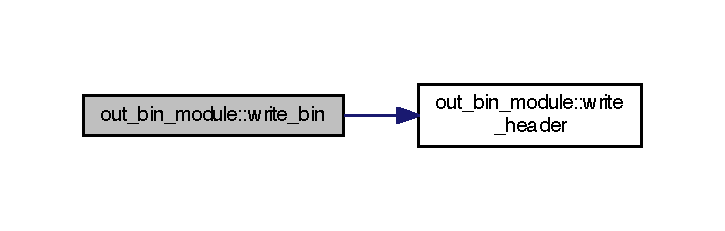
\includegraphics[width=348pt]{namespaceout__bin__module_ac5772f05ffdd0227d2fc17e27beb0f59_cgraph}
\end{center}
\end{figure}


\hypertarget{namespaceout__bin__module_a6e5fb4bb1cc6f0a15ce591a3b1014d8d}{}\index{out\+\_\+bin\+\_\+module@{out\+\_\+bin\+\_\+module}!write\+\_\+header@{write\+\_\+header}}
\index{write\+\_\+header@{write\+\_\+header}!out\+\_\+bin\+\_\+module@{out\+\_\+bin\+\_\+module}}
\subsubsection[{write\+\_\+header}]{\setlength{\rightskip}{0pt plus 5cm}subroutine out\+\_\+bin\+\_\+module\+::write\+\_\+header (
\begin{DoxyParamCaption}
\item[{integer, intent(in)}]{unit, }
\item[{integer, intent(in)}]{neq\+\_\+out, }
\item[{integer, intent(in)}]{nghost\+\_\+out}
\end{DoxyParamCaption}
)}\label{namespaceout__bin__module_a6e5fb4bb1cc6f0a15ce591a3b1014d8d}
Writes header for binary input 
\begin{DoxyParams}{Parameters}
{\em integer} & \mbox{[}in\mbox{]} unit \+: number of logical unit \\
\hline
\end{DoxyParams}


Definition at line 43 of file Out\+\_\+\+B\+I\+N\+\_\+\+Module.\+f90.


\hypertarget{namespaceout__silo__module}{}\section{out\+\_\+silo\+\_\+module Module Reference}
\label{namespaceout__silo__module}\index{out\+\_\+silo\+\_\+module@{out\+\_\+silo\+\_\+module}}


Output in Silo (+\+H\+D\+F5) Format.  


\subsection*{Functions/\+Subroutines}
\begin{DoxyCompactItemize}
\item 
subroutine \hyperlink{namespaceout__silo__module_acfa5a749647a6a7c95e48e3ad58e4139}{writeblocks} (itprint)
\begin{DoxyCompactList}\small\item\em Writes Data, one file per processor. \end{DoxyCompactList}\item 
subroutine \hyperlink{namespaceout__silo__module_aa984d6044bf34559a87a9020c4a07c3a}{writemaster} (itprint)
\begin{DoxyCompactList}\small\item\em Writes the Master File. \end{DoxyCompactList}\item 
subroutine \hyperlink{namespaceout__silo__module_a65763f848b9b5da2a20d8b55f53f8515}{outputsilo} (itprint)
\begin{DoxyCompactList}\small\item\em Upper level wrapper. \end{DoxyCompactList}\end{DoxyCompactItemize}


\subsection{Detailed Description}
This module writes the ouput in S\+I\+L\+O (H\+D\+F5) format 

\subsection{Function/\+Subroutine Documentation}
\hypertarget{namespaceout__silo__module_a65763f848b9b5da2a20d8b55f53f8515}{}\index{out\+\_\+silo\+\_\+module@{out\+\_\+silo\+\_\+module}!outputsilo@{outputsilo}}
\index{outputsilo@{outputsilo}!out\+\_\+silo\+\_\+module@{out\+\_\+silo\+\_\+module}}
\subsubsection[{outputsilo}]{\setlength{\rightskip}{0pt plus 5cm}subroutine out\+\_\+silo\+\_\+module\+::outputsilo (
\begin{DoxyParamCaption}
\item[{integer, intent(in)}]{itprint}
\end{DoxyParamCaption}
)}\label{namespaceout__silo__module_a65763f848b9b5da2a20d8b55f53f8515}
Upper level wrapper for the S\+I\+L\+O output 
\begin{DoxyParams}{Parameters}
{\em integer} & \mbox{[}in\mbox{]} itprint \+: number of output \\
\hline
\end{DoxyParams}


Definition at line 347 of file Out\+\_\+\+Silo\+\_\+\+Module.\+f90.



Here is the call graph for this function\+:\nopagebreak
\begin{figure}[H]
\begin{center}
\leavevmode
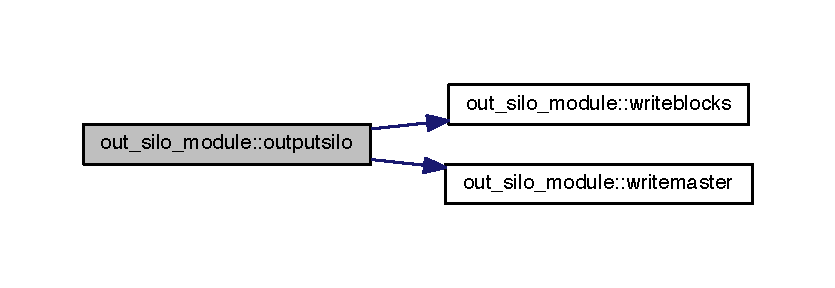
\includegraphics[width=350pt]{namespaceout__silo__module_a65763f848b9b5da2a20d8b55f53f8515_cgraph}
\end{center}
\end{figure}


\hypertarget{namespaceout__silo__module_acfa5a749647a6a7c95e48e3ad58e4139}{}\index{out\+\_\+silo\+\_\+module@{out\+\_\+silo\+\_\+module}!writeblocks@{writeblocks}}
\index{writeblocks@{writeblocks}!out\+\_\+silo\+\_\+module@{out\+\_\+silo\+\_\+module}}
\subsubsection[{writeblocks}]{\setlength{\rightskip}{0pt plus 5cm}subroutine out\+\_\+silo\+\_\+module\+::writeblocks (
\begin{DoxyParamCaption}
\item[{integer, intent(in)}]{itprint}
\end{DoxyParamCaption}
)}\label{namespaceout__silo__module_acfa5a749647a6a7c95e48e3ad58e4139}
Writes Data in silo format one file per processor 
\begin{DoxyParams}{Parameters}
{\em integer} & \mbox{[}in\mbox{]} itprint \+: number of output \\
\hline
\end{DoxyParams}


Definition at line 44 of file Out\+\_\+\+Silo\+\_\+\+Module.\+f90.

\hypertarget{namespaceout__silo__module_aa984d6044bf34559a87a9020c4a07c3a}{}\index{out\+\_\+silo\+\_\+module@{out\+\_\+silo\+\_\+module}!writemaster@{writemaster}}
\index{writemaster@{writemaster}!out\+\_\+silo\+\_\+module@{out\+\_\+silo\+\_\+module}}
\subsubsection[{writemaster}]{\setlength{\rightskip}{0pt plus 5cm}subroutine out\+\_\+silo\+\_\+module\+::writemaster (
\begin{DoxyParamCaption}
\item[{integer, intent(in)}]{itprint}
\end{DoxyParamCaption}
)}\label{namespaceout__silo__module_aa984d6044bf34559a87a9020c4a07c3a}
Writes the master file with the metadata and multivars 
\begin{DoxyParams}{Parameters}
{\em integer} & \mbox{[}in\mbox{]} itprint \+: number of output \\
\hline
\end{DoxyParams}


Definition at line 198 of file Out\+\_\+\+Silo\+\_\+\+Module.\+f90.


\hypertarget{namespaceout__vtk__module}{}\section{out\+\_\+vtk\+\_\+module Module Reference}
\label{namespaceout__vtk__module}\index{out\+\_\+vtk\+\_\+module@{out\+\_\+vtk\+\_\+module}}


Output in V\+T\+K format.  


\subsection*{Functions/\+Subroutines}
\begin{DoxyCompactItemize}
\item 
subroutine \hyperlink{namespaceout__vtk__module_ac34f91e1b74dd533461d7ead905bf937}{write\+\_\+vtk} (itprint)
\begin{DoxyCompactList}\small\item\em Writes Data, one file per processor. \end{DoxyCompactList}\end{DoxyCompactItemize}


\subsection{Detailed Description}
This module writes the ouput in V\+T\+K format 

\subsection{Function/\+Subroutine Documentation}
\hypertarget{namespaceout__vtk__module_ac34f91e1b74dd533461d7ead905bf937}{}\index{out\+\_\+vtk\+\_\+module@{out\+\_\+vtk\+\_\+module}!write\+\_\+vtk@{write\+\_\+vtk}}
\index{write\+\_\+vtk@{write\+\_\+vtk}!out\+\_\+vtk\+\_\+module@{out\+\_\+vtk\+\_\+module}}
\subsubsection[{write\+\_\+vtk}]{\setlength{\rightskip}{0pt plus 5cm}subroutine out\+\_\+vtk\+\_\+module\+::write\+\_\+vtk (
\begin{DoxyParamCaption}
\item[{integer, intent(in)}]{itprint}
\end{DoxyParamCaption}
)}\label{namespaceout__vtk__module_ac34f91e1b74dd533461d7ead905bf937}
Writes Data in V\+T\+K format one file per processor 
\begin{DoxyParams}{Parameters}
{\em integer} & \mbox{[}in\mbox{]} itprint \+: number of output \\
\hline
\end{DoxyParams}


Definition at line 43 of file Out\+\_\+\+V\+T\+K\+\_\+\+Module.\+f90.



Here is the call graph for this function\+:\nopagebreak
\begin{figure}[H]
\begin{center}
\leavevmode
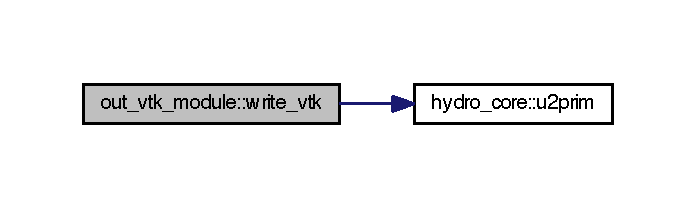
\includegraphics[width=334pt]{namespaceout__vtk__module_ac34f91e1b74dd533461d7ead905bf937_cgraph}
\end{center}
\end{figure}



\hypertarget{namespaceoutput}{}\section{output Module Reference}
\label{namespaceoutput}\index{output@{output}}


Writes output.  


\subsection*{Functions/\+Subroutines}
\begin{DoxyCompactItemize}
\item 
subroutine \hyperlink{namespaceoutput_a9a6f65196f6b514f504929c9e1f7582f}{write\+\_\+output} (itprint)
\begin{DoxyCompactList}\small\item\em Writes output. \end{DoxyCompactList}\end{DoxyCompactItemize}


\subsection{Detailed Description}
This module writes the ouput in the formats specified in the makefile 

\subsection{Function/\+Subroutine Documentation}
\hypertarget{namespaceoutput_a9a6f65196f6b514f504929c9e1f7582f}{}\index{output@{output}!write\+\_\+output@{write\+\_\+output}}
\index{write\+\_\+output@{write\+\_\+output}!output@{output}}
\subsubsection[{write\+\_\+output}]{\setlength{\rightskip}{0pt plus 5cm}subroutine output\+::write\+\_\+output (
\begin{DoxyParamCaption}
\item[{integer, intent(in)}]{itprint}
\end{DoxyParamCaption}
)}\label{namespaceoutput_a9a6f65196f6b514f504929c9e1f7582f}
Writes output, the format is chosen in makefile ~\newline
 Supported formats are $\ast$.bin and V\+T\+K (both B\+I\+N\+A\+R\+Y), Silo (+hdf5) 
\begin{DoxyParams}{Parameters}
{\em integer} & \mbox{[}in\mbox{]} itprint \+: number of output \\
\hline
\end{DoxyParams}


Definition at line 42 of file output.\+f90.



Here is the call graph for this function\+:\nopagebreak
\begin{figure}[H]
\begin{center}
\leavevmode
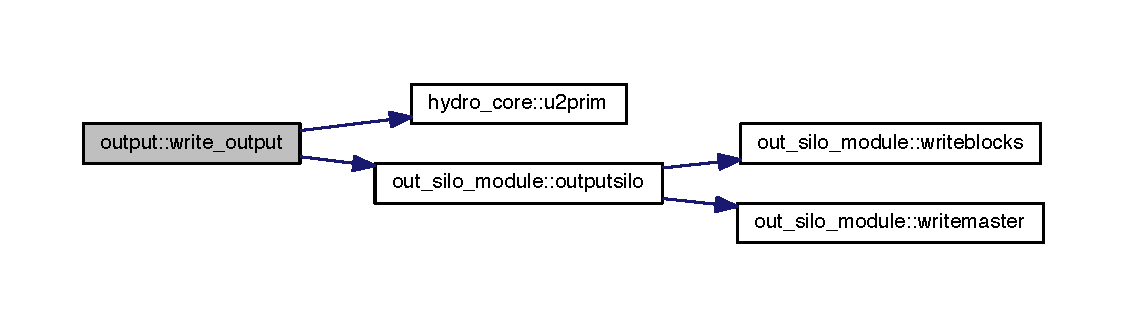
\includegraphics[width=350pt]{namespaceoutput_a9a6f65196f6b514f504929c9e1f7582f_cgraph}
\end{center}
\end{figure}



\hypertarget{namespacesources}{}\section{sources Module Reference}
\label{namespacesources}\index{sources@{sources}}


Adds source terms.  


\subsection*{Functions/\+Subroutines}
\begin{DoxyCompactItemize}
\item 
subroutine \hyperlink{namespacesources_a378a8116ae16db2efa853343f88156d3}{getpos} (i, j, k, x, y, z, r)
\begin{DoxyCompactList}\small\item\em Gets position in the grid. \end{DoxyCompactList}\item 
subroutine \hyperlink{namespacesources_aef9f6ca4bc770f0e768dbbba91b67415}{grav\+\_\+source} (xc, yc, zc, pp, s)
\begin{DoxyCompactList}\small\item\em Gravity due to point sources. \end{DoxyCompactList}\item 
subroutine \hyperlink{namespacesources_a36b548c9c578b74c5f439ffaec7d3a9a}{radpress\+\_\+source} (i, j, k, xc, yc, zc, rc, pp, s)
\begin{DoxyCompactList}\small\item\em Radiation pressure force. \end{DoxyCompactList}\item 
subroutine \hyperlink{namespacesources_a0478795277b4f25ec62d8e3e1f06611e}{divergence\+\_\+b} (i, j, k, d)
\begin{DoxyCompactList}\small\item\em Computes div(\+B) \end{DoxyCompactList}\item 
subroutine \hyperlink{namespacesources_a9c2d37de3b878eff7693a25d3dc3fe91}{divbcorr\+\_\+source} (i, j, k, pp, s)
\begin{DoxyCompactList}\small\item\em 8 Wave source terms for div(\+B) correction \end{DoxyCompactList}\item 
subroutine \hyperlink{namespacesources_a6a66dd1f8baf424ff64a30112f39c632}{source} (i, j, k, prim, s)
\begin{DoxyCompactList}\small\item\em Upper level wrapper for sources. \end{DoxyCompactList}\end{DoxyCompactItemize}


\subsection{Detailed Description}
This module adds the source terms from gravity, radiation pressure (not fully tested), and div(\+B) cleaning if the 8 wave scheme is used 

\subsection{Function/\+Subroutine Documentation}
\hypertarget{namespacesources_a9c2d37de3b878eff7693a25d3dc3fe91}{}\index{sources@{sources}!divbcorr\+\_\+source@{divbcorr\+\_\+source}}
\index{divbcorr\+\_\+source@{divbcorr\+\_\+source}!sources@{sources}}
\subsubsection[{divbcorr\+\_\+source}]{\setlength{\rightskip}{0pt plus 5cm}subroutine sources\+::divbcorr\+\_\+source (
\begin{DoxyParamCaption}
\item[{integer, intent(in)}]{i, }
\item[{integer, intent(in)}]{j, }
\item[{integer, intent(in)}]{k, }
\item[{real, dimension(neq), intent(in)}]{pp, }
\item[{real, dimension(neq), intent(inout)}]{s}
\end{DoxyParamCaption}
)}\label{namespacesources_a9c2d37de3b878eff7693a25d3dc3fe91}
Adds terms proportional to div B in Faraday\textquotesingle{}s Law, momentum equationand energy equation as propoes in Powell et al. 1999 
\begin{DoxyParams}{Parameters}
{\em integer} & \mbox{[}in\mbox{]} i \+: cell index in the X direction \\
\hline
{\em integer} & \mbox{[}in\mbox{]} j \+: cell index in the Y direction \\
\hline
{\em integer} & \mbox{[}in\mbox{]} k \+: cell index in the Z direction \\
\hline
{\em real} & \mbox{[}in\mbox{]} pp(neq) \+: vector of primitive variables \\
\hline
{\em real} & \mbox{[}out\mbox{]} s(neq) \+: vector with source terms \\
\hline
\end{DoxyParams}


Definition at line 201 of file sources.\+f90.



Here is the call graph for this function\+:
% FIG 0


\hypertarget{namespacesources_a0478795277b4f25ec62d8e3e1f06611e}{}\index{sources@{sources}!divergence\+\_\+b@{divergence\+\_\+b}}
\index{divergence\+\_\+b@{divergence\+\_\+b}!sources@{sources}}
\subsubsection[{divergence\+\_\+b}]{\setlength{\rightskip}{0pt plus 5cm}subroutine sources\+::divergence\+\_\+b (
\begin{DoxyParamCaption}
\item[{integer, intent(in)}]{i, }
\item[{integer, intent(in)}]{j, }
\item[{integer, intent(in)}]{k, }
\item[{real, intent(out)}]{d}
\end{DoxyParamCaption}
)}\label{namespacesources_a0478795277b4f25ec62d8e3e1f06611e}
Computes div(\+B) 
\begin{DoxyParams}{Parameters}
{\em integer} & \mbox{[}in\mbox{]} i \+: cell index in the X direction \\
\hline
{\em integer} & \mbox{[}in\mbox{]} j \+: cell index in the Y direction \\
\hline
{\em integer} & \mbox{[}in\mbox{]} k \+: cell index in the Z direction \\
\hline
{\em real} & \mbox{[}out\mbox{]} d \+:\+: div(\+B) \\
\hline
\end{DoxyParams}


Definition at line 178 of file sources.\+f90.

\hypertarget{namespacesources_a378a8116ae16db2efa853343f88156d3}{}\index{sources@{sources}!getpos@{getpos}}
\index{getpos@{getpos}!sources@{sources}}
\subsubsection[{getpos}]{\setlength{\rightskip}{0pt plus 5cm}subroutine sources\+::getpos (
\begin{DoxyParamCaption}
\item[{integer, intent(in)}]{i, }
\item[{integer, intent(in)}]{j, }
\item[{integer, intent(in)}]{k, }
\item[{real, intent(out)}]{x, }
\item[{real, intent(out)}]{y, }
\item[{real, intent(out)}]{z, }
\item[{real, intent(out)}]{r}
\end{DoxyParamCaption}
)}\label{namespacesources_a378a8116ae16db2efa853343f88156d3}
Gets the position and spherical radius calculated with respect to the center of the grid 
\begin{DoxyParams}{Parameters}
{\em integer} & \mbox{[}in\mbox{]} i \+: index in the X direction \\
\hline
{\em integer} & \mbox{[}in\mbox{]} j \+: index in the Y direction \\
\hline
{\em integer} & \mbox{[}in\mbox{]} k \+: index in the Z direction \\
\hline
{\em real} & \mbox{[}out\mbox{]} x \+: X position form the center of the grid (code units) \\
\hline
{\em real} & \mbox{[}out\mbox{]} y \+: Y position form the center of the grid (code units) \\
\hline
{\em real} & \mbox{[}out\mbox{]} z \+: Z position form the center of the grid (code units) \\
\hline
{\em real} & \mbox{[}out\mbox{]} r \+: Spherical radius form the center of the grid (code units) \\
\hline
\end{DoxyParams}


Definition at line 55 of file sources.\+f90.

\hypertarget{namespacesources_aef9f6ca4bc770f0e768dbbba91b67415}{}\index{sources@{sources}!grav\+\_\+source@{grav\+\_\+source}}
\index{grav\+\_\+source@{grav\+\_\+source}!sources@{sources}}
\subsubsection[{grav\+\_\+source}]{\setlength{\rightskip}{0pt plus 5cm}subroutine sources\+::grav\+\_\+source (
\begin{DoxyParamCaption}
\item[{real, intent(in)}]{xc, }
\item[{real, intent(in)}]{yc, }
\item[{real, intent(in)}]{zc, }
\item[{real, dimension(neq), intent(in)}]{pp, }
\item[{real, dimension(neq), intent(inout)}]{s}
\end{DoxyParamCaption}
)}\label{namespacesources_aef9f6ca4bc770f0e768dbbba91b67415}
Adds the gravitational force due to point particles, at this moment is fixed to two point sources (exoplanet) 
\begin{DoxyParams}{Parameters}
{\em real} & \mbox{[}in\mbox{]} xc \+: X position of the cell \\
\hline
{\em real} & \mbox{[}in\mbox{]} yc \+: Y position of the cell \\
\hline
{\em real} & \mbox{[}in\mbox{]} zc \+: Z position of the cell \\
\hline
{\em real} & \mbox{[}in\mbox{]} pp(neq) \+: vector of primitive variables \\
\hline
{\em real} & \mbox{[}out\mbox{]} s(neq) \+: vector with source terms \\
\hline
\end{DoxyParams}


Definition at line 82 of file sources.\+f90.

\hypertarget{namespacesources_a36b548c9c578b74c5f439ffaec7d3a9a}{}\index{sources@{sources}!radpress\+\_\+source@{radpress\+\_\+source}}
\index{radpress\+\_\+source@{radpress\+\_\+source}!sources@{sources}}
\subsubsection[{radpress\+\_\+source}]{\setlength{\rightskip}{0pt plus 5cm}subroutine sources\+::radpress\+\_\+source (
\begin{DoxyParamCaption}
\item[{integer, intent(in)}]{i, }
\item[{integer, intent(in)}]{j, }
\item[{integer, intent(in)}]{k, }
\item[{real, intent(in)}]{xc, }
\item[{real, intent(in)}]{yc, }
\item[{real, intent(in)}]{zc, }
\item[{real, intent(in)}]{rc, }
\item[{real, dimension(neq), intent(in)}]{pp, }
\item[{real, dimension(neq), intent(inout)}]{s}
\end{DoxyParamCaption}
)}\label{namespacesources_a36b548c9c578b74c5f439ffaec7d3a9a}
Adds the radiaiton pressure force due to photo-\/ionization 
\begin{DoxyParams}{Parameters}
{\em integer} & \mbox{[}in\mbox{]} i \+: cell index in the X direction \\
\hline
{\em integer} & \mbox{[}in\mbox{]} j \+: cell index in the Y direction \\
\hline
{\em integer} & \mbox{[}in\mbox{]} k \+: cell index in the Z direction \\
\hline
{\em real} & \mbox{[}in\mbox{]} xc \+: X position of the cell \\
\hline
{\em real} & \mbox{[}in\mbox{]} yc \+: Y position of the cell \\
\hline
{\em real} & \mbox{[}in\mbox{]} zc \+: Z position of the cell \\
\hline
{\em reak} & \mbox{[}in\mbox{]} rc \+: $ \sqrt{x^2+y^2+z^2} $ \\
\hline
{\em real} & \mbox{[}in\mbox{]} pp(neq) \+: vector of primitive variables \\
\hline
{\em real} & \mbox{[}out\mbox{]} s(neq) \+: vector with source terms \\
\hline
\end{DoxyParams}


Definition at line 140 of file sources.\+f90.

\hypertarget{namespacesources_a6a66dd1f8baf424ff64a30112f39c632}{}\index{sources@{sources}!source@{source}}
\index{source@{source}!sources@{sources}}
\subsubsection[{source}]{\setlength{\rightskip}{0pt plus 5cm}subroutine sources\+::source (
\begin{DoxyParamCaption}
\item[{integer, intent(in)}]{i, }
\item[{integer, intent(in)}]{j, }
\item[{integer, intent(in)}]{k, }
\item[{real, dimension(neq), intent(in)}]{prim, }
\item[{real, dimension(neq), intent(out)}]{s}
\end{DoxyParamCaption}
)}\label{namespacesources_a6a66dd1f8baf424ff64a30112f39c632}
Upper level wrapper for sources ~\newline
 Main driver, this is called from the upwind stepping 
\begin{DoxyParams}{Parameters}
{\em integer} & \mbox{[}in\mbox{]} i \+: cell index in the X direction \\
\hline
{\em integer} & \mbox{[}in\mbox{]} j \+: cell index in the Y direction \\
\hline
{\em integer} & \mbox{[}in\mbox{]} k \+: cell index in the Z direction \\
\hline
{\em real} & \mbox{[}in\mbox{]} prim(neq) \+: vector of primitive variables \\
\hline
{\em real} & \mbox{[}out\mbox{]} s(neq) \+: vector with source terms\textquotesingle{} \\
\hline
\end{DoxyParams}


Definition at line 240 of file sources.\+f90.



Here is the call graph for this function\+:
% FIG 1



\hypertarget{namespacethermal__cond}{}\section{thermal\+\_\+cond Module Reference}
\label{namespacethermal__cond}\index{thermal\+\_\+cond@{thermal\+\_\+cond}}


Adds thermal conducion.  


\subsection*{Functions/\+Subroutines}
\begin{DoxyCompactItemize}
\item 
subroutine \hyperlink{namespacethermal__cond_ac611766519a4602033c83e3ed5ae3c00}{init\+\_\+thermal\+\_\+cond} ()
\begin{DoxyCompactList}\small\item\em Intializes Temperature array. \end{DoxyCompactList}\item 
subroutine \hyperlink{namespacethermal__cond_a074d4829b3477fa8003983819e77523d}{get\+\_\+dt\+\_\+cond} (dt)
\begin{DoxyCompactList}\small\item\em computes conduction timescale \end{DoxyCompactList}\item 
subroutine \hyperlink{namespacethermal__cond_a5283f7a2b8b4a4226ce624fb49445f43}{progress} (j, tot)
\begin{DoxyCompactList}\small\item\em Progress bar. \end{DoxyCompactList}\item 
real function \hyperlink{namespacethermal__cond_ab3978fb62e485cf71d7c83e779e92615}{ksp} (T)
\begin{DoxyCompactList}\small\item\em Spitzer conductivity. \end{DoxyCompactList}\item 
real function \hyperlink{namespacethermal__cond_a8205274631d6cb4d36ffc0937aa88a74}{ksp\+\_\+parl} (xtemp)
\begin{DoxyCompactList}\small\item\em Spitzer parallel conductivity. \end{DoxyCompactList}\item 
real function \hyperlink{namespacethermal__cond_adfd8867a0fc7fe02a35a41000e36f9bf}{ksp\+\_\+perp} (xtemp, xdens, B2)
\begin{DoxyCompactList}\small\item\em Spitzer perpendicular conductivity. \end{DoxyCompactList}\item 
subroutine \hyperlink{namespacethermal__cond_abc5c4fc622aea2f85fc5a0c2fee333bc}{heatfluxes} ()
\begin{DoxyCompactList}\small\item\em Returns Heat Fluxes. \end{DoxyCompactList}\item 
subroutine \hyperlink{namespacethermal__cond_aab43551b6a0d4b5894c07b510e4571d7}{mhd\+\_\+heatfluxes} ()
\begin{DoxyCompactList}\small\item\em Returns Heat Fluxes with anisotropic thermal conduction. \end{DoxyCompactList}\item 
subroutine \hyperlink{namespacethermal__cond_a55e65df0c700580f8af0a090063d2e32}{thermal\+\_\+bounds} ()
\begin{DoxyCompactList}\small\item\em Exchanges ghost cells for energy only. \end{DoxyCompactList}\item 
real function \hyperlink{namespacethermal__cond_a535cc1746914d413d4978aeda7b8fc06}{superstep} (N, \hyperlink{namespacethermal__cond_a53b14d15ce11990f6453a335c81d1728}{snu})
\begin{DoxyCompactList}\small\item\em Length of superstep. \end{DoxyCompactList}\item 
real function \hyperlink{namespacethermal__cond_a782aaba01217281f2aa57dcc955fd294}{substep} (j, N, \hyperlink{namespacethermal__cond_a38896e6bbd3b053ca066e407e4b3817f}{nu})
\begin{DoxyCompactList}\small\item\em Size of substep j. \end{DoxyCompactList}\item 
subroutine \hyperlink{namespacethermal__cond_a4c74dc0fd6a165d0fea419b560943701}{st\+\_\+steps} (fs, Ns, fstep)
\begin{DoxyCompactList}\small\item\em Returns the number of Supersteps. \end{DoxyCompactList}\item 
subroutine \hyperlink{namespacethermal__cond_a4b579df47b3bf4622a3ab51f57aa436b}{thermal\+\_\+conduction} ()
\begin{DoxyCompactList}\small\item\em Upper level wrapper for thermal conduction. \end{DoxyCompactList}\end{DoxyCompactItemize}
\subsection*{Variables}
\begin{DoxyCompactItemize}
\item 
\hypertarget{namespacethermal__cond_a37c3e000231baaaa4668f7c05f021ce0}{}real, parameter \hyperlink{namespacethermal__cond_a37c3e000231baaaa4668f7c05f021ce0}{ph} =0.\+4\label{namespacethermal__cond_a37c3e000231baaaa4668f7c05f021ce0}

\begin{DoxyCompactList}\small\item\em Parameter for the sturated regime in Mc\+Kee. \end{DoxyCompactList}\item 
\hypertarget{namespacethermal__cond_a38896e6bbd3b053ca066e407e4b3817f}{}real, parameter \hyperlink{namespacethermal__cond_a38896e6bbd3b053ca066e407e4b3817f}{nu} =0.\+01\label{namespacethermal__cond_a38896e6bbd3b053ca066e407e4b3817f}

\begin{DoxyCompactList}\small\item\em Super-\/stepping da\+M\+P\+I\+\_\+\+N\+Bg factor. \end{DoxyCompactList}\item 
\hypertarget{namespacethermal__cond_a53b14d15ce11990f6453a335c81d1728}{}real, parameter \hyperlink{namespacethermal__cond_a53b14d15ce11990f6453a335c81d1728}{snu} =sqrt(\hyperlink{namespacethermal__cond_a38896e6bbd3b053ca066e407e4b3817f}{nu})\label{namespacethermal__cond_a53b14d15ce11990f6453a335c81d1728}

\begin{DoxyCompactList}\small\item\em Sqrt of damping factor. \end{DoxyCompactList}\item 
\hypertarget{namespacethermal__cond_a5420f28be46174eb6852f14281ec7ace}{}integer, parameter \hyperlink{namespacethermal__cond_a5420f28be46174eb6852f14281ec7ace}{max\+\_\+iter} = 100\label{namespacethermal__cond_a5420f28be46174eb6852f14281ec7ace}

\begin{DoxyCompactList}\small\item\em Maximum number of iterations. \end{DoxyCompactList}\item 
\hypertarget{namespacethermal__cond_ae13a8d994e65b9e57ebb80e892c72aac}{}real, parameter \hyperlink{namespacethermal__cond_ae13a8d994e65b9e57ebb80e892c72aac}{tstep\+\_\+red\+\_\+factor} =0.\+25\label{namespacethermal__cond_ae13a8d994e65b9e57ebb80e892c72aac}

\begin{DoxyCompactList}\small\item\em timestep reduction factor for the conduction \end{DoxyCompactList}\item 
\hypertarget{namespacethermal__cond_a0d692500ab9d6becafcf89d733d3f76f}{}real \hyperlink{namespacethermal__cond_a0d692500ab9d6becafcf89d733d3f76f}{dt\+\_\+cond}\label{namespacethermal__cond_a0d692500ab9d6becafcf89d733d3f76f}

\begin{DoxyCompactList}\small\item\em conduction timestep \end{DoxyCompactList}\item 
\hypertarget{namespacethermal__cond_a03140c73c7461f1882cd286b3e378abc}{}integer \hyperlink{namespacethermal__cond_a03140c73c7461f1882cd286b3e378abc}{tc\+\_\+log}\label{namespacethermal__cond_a03140c73c7461f1882cd286b3e378abc}

\begin{DoxyCompactList}\small\item\em loical unit to write T\+C log \end{DoxyCompactList}\end{DoxyCompactItemize}


\subsection{Detailed Description}
Adds a thermal conduction term, affects both the primitive and conserved variables 

\subsection{Function/\+Subroutine Documentation}
\hypertarget{namespacethermal__cond_a074d4829b3477fa8003983819e77523d}{}\index{thermal\+\_\+cond@{thermal\+\_\+cond}!get\+\_\+dt\+\_\+cond@{get\+\_\+dt\+\_\+cond}}
\index{get\+\_\+dt\+\_\+cond@{get\+\_\+dt\+\_\+cond}!thermal\+\_\+cond@{thermal\+\_\+cond}}
\subsubsection[{get\+\_\+dt\+\_\+cond}]{\setlength{\rightskip}{0pt plus 5cm}subroutine thermal\+\_\+cond\+::get\+\_\+dt\+\_\+cond (
\begin{DoxyParamCaption}
\item[{real, intent(out)}]{dt}
\end{DoxyParamCaption}
)}\label{namespacethermal__cond_a074d4829b3477fa8003983819e77523d}
computes conduction timescale (in seconds) 
\begin{DoxyParams}{Parameters}
{\em real} & \mbox{[}out\mbox{]} dt \+:\+: conduction timescale \\
\hline
\end{DoxyParams}


Definition at line 83 of file thermal\+\_\+cond.\+f90.



Here is the call graph for this function\+:\nopagebreak
\begin{figure}[H]
\begin{center}
\leavevmode
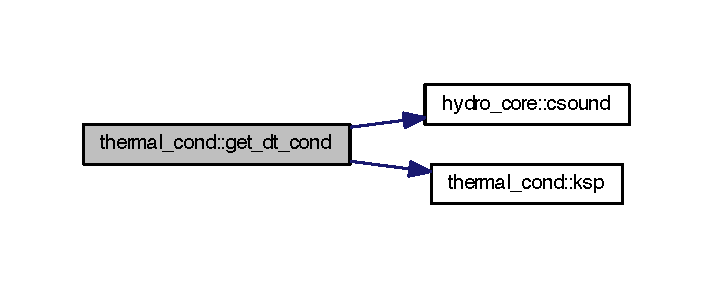
\includegraphics[width=342pt]{namespacethermal__cond_a074d4829b3477fa8003983819e77523d_cgraph}
\end{center}
\end{figure}


\hypertarget{namespacethermal__cond_abc5c4fc622aea2f85fc5a0c2fee333bc}{}\index{thermal\+\_\+cond@{thermal\+\_\+cond}!heatfluxes@{heatfluxes}}
\index{heatfluxes@{heatfluxes}!thermal\+\_\+cond@{thermal\+\_\+cond}}
\subsubsection[{heatfluxes}]{\setlength{\rightskip}{0pt plus 5cm}subroutine thermal\+\_\+cond\+::heatfluxes (
\begin{DoxyParamCaption}
{}
\end{DoxyParamCaption}
)}\label{namespacethermal__cond_abc5c4fc622aea2f85fc5a0c2fee333bc}
Heat flux, if saturation enabled it takes minimum of the Spitzer and the saturated value ~\newline
 The result is stored in the 5th component of global the F,G,H fluxes (in cgs, conversion is done in dt product) 

Definition at line 194 of file thermal\+\_\+cond.\+f90.



Here is the call graph for this function\+:\nopagebreak
\begin{figure}[H]
\begin{center}
\leavevmode
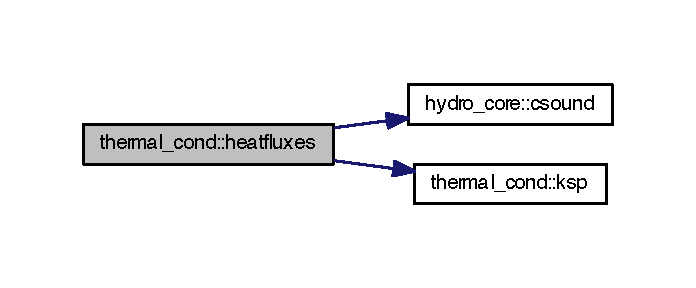
\includegraphics[width=334pt]{namespacethermal__cond_abc5c4fc622aea2f85fc5a0c2fee333bc_cgraph}
\end{center}
\end{figure}


\hypertarget{namespacethermal__cond_ac611766519a4602033c83e3ed5ae3c00}{}\index{thermal\+\_\+cond@{thermal\+\_\+cond}!init\+\_\+thermal\+\_\+cond@{init\+\_\+thermal\+\_\+cond}}
\index{init\+\_\+thermal\+\_\+cond@{init\+\_\+thermal\+\_\+cond}!thermal\+\_\+cond@{thermal\+\_\+cond}}
\subsubsection[{init\+\_\+thermal\+\_\+cond}]{\setlength{\rightskip}{0pt plus 5cm}subroutine thermal\+\_\+cond\+::init\+\_\+thermal\+\_\+cond (
\begin{DoxyParamCaption}
{}
\end{DoxyParamCaption}
)}\label{namespacethermal__cond_ac611766519a4602033c83e3ed5ae3c00}
Intializes Temperature array (to resolve dependencies it was moved to the globals module) 

Definition at line 55 of file thermal\+\_\+cond.\+f90.

\hypertarget{namespacethermal__cond_ab3978fb62e485cf71d7c83e779e92615}{}\index{thermal\+\_\+cond@{thermal\+\_\+cond}!ksp@{ksp}}
\index{ksp@{ksp}!thermal\+\_\+cond@{thermal\+\_\+cond}}
\subsubsection[{ksp}]{\setlength{\rightskip}{0pt plus 5cm}real function thermal\+\_\+cond\+::ksp (
\begin{DoxyParamCaption}
\item[{real, intent(in)}]{T}
\end{DoxyParamCaption}
)}\label{namespacethermal__cond_ab3978fb62e485cf71d7c83e779e92615}
Computes the Spitzer conductivity 
\begin{DoxyParams}{Parameters}
{\em real} & \mbox{[}in\mbox{]} T \+: temperature \mbox{[}K\mbox{]} \\
\hline
\end{DoxyParams}


Definition at line 147 of file thermal\+\_\+cond.\+f90.

\hypertarget{namespacethermal__cond_a8205274631d6cb4d36ffc0937aa88a74}{}\index{thermal\+\_\+cond@{thermal\+\_\+cond}!ksp\+\_\+parl@{ksp\+\_\+parl}}
\index{ksp\+\_\+parl@{ksp\+\_\+parl}!thermal\+\_\+cond@{thermal\+\_\+cond}}
\subsubsection[{ksp\+\_\+parl}]{\setlength{\rightskip}{0pt plus 5cm}real function thermal\+\_\+cond\+::ksp\+\_\+parl (
\begin{DoxyParamCaption}
\item[{real, intent(in)}]{xtemp}
\end{DoxyParamCaption}
)}\label{namespacethermal__cond_a8205274631d6cb4d36ffc0937aa88a74}
Computes the Spitzer conductivity parallel to B 
\begin{DoxyParams}{Parameters}
{\em real} & \mbox{[}in\mbox{]} T \+: temperature \mbox{[}K\mbox{]} \\
\hline
\end{DoxyParams}


Definition at line 162 of file thermal\+\_\+cond.\+f90.

\hypertarget{namespacethermal__cond_adfd8867a0fc7fe02a35a41000e36f9bf}{}\index{thermal\+\_\+cond@{thermal\+\_\+cond}!ksp\+\_\+perp@{ksp\+\_\+perp}}
\index{ksp\+\_\+perp@{ksp\+\_\+perp}!thermal\+\_\+cond@{thermal\+\_\+cond}}
\subsubsection[{ksp\+\_\+perp}]{\setlength{\rightskip}{0pt plus 5cm}real function thermal\+\_\+cond\+::ksp\+\_\+perp (
\begin{DoxyParamCaption}
\item[{real, intent(in)}]{xtemp, }
\item[{real, intent(in)}]{xdens, }
\item[{real, intent(in)}]{B2}
\end{DoxyParamCaption}
)}\label{namespacethermal__cond_adfd8867a0fc7fe02a35a41000e36f9bf}
Computes the Spitzer conductivity perpendicular to B 
\begin{DoxyParams}{Parameters}
{\em real} & \mbox{[}in\mbox{]} T \+: temperature \mbox{[}K\mbox{]} \\
\hline
\end{DoxyParams}


Definition at line 177 of file thermal\+\_\+cond.\+f90.

\hypertarget{namespacethermal__cond_aab43551b6a0d4b5894c07b510e4571d7}{}\index{thermal\+\_\+cond@{thermal\+\_\+cond}!mhd\+\_\+heatfluxes@{mhd\+\_\+heatfluxes}}
\index{mhd\+\_\+heatfluxes@{mhd\+\_\+heatfluxes}!thermal\+\_\+cond@{thermal\+\_\+cond}}
\subsubsection[{mhd\+\_\+heatfluxes}]{\setlength{\rightskip}{0pt plus 5cm}subroutine thermal\+\_\+cond\+::mhd\+\_\+heatfluxes (
\begin{DoxyParamCaption}
{}
\end{DoxyParamCaption}
)}\label{namespacethermal__cond_aab43551b6a0d4b5894c07b510e4571d7}
Heat flux, if sturation enabled takes minimum of the Spitzer and the saturated value ~\newline
 The result is stored in the 5th component of global the F,G,H fluxes (in cgs, conversion is done in dt product) 

Definition at line 285 of file thermal\+\_\+cond.\+f90.



Here is the call graph for this function\+:
% FIG 0


\hypertarget{namespacethermal__cond_a5283f7a2b8b4a4226ce624fb49445f43}{}\index{thermal\+\_\+cond@{thermal\+\_\+cond}!progress@{progress}}
\index{progress@{progress}!thermal\+\_\+cond@{thermal\+\_\+cond}}
\subsubsection[{progress}]{\setlength{\rightskip}{0pt plus 5cm}subroutine thermal\+\_\+cond\+::progress (
\begin{DoxyParamCaption}
\item[{integer(kind=4)}]{j, }
\item[{integer(kind=4), intent(in)}]{tot}
\end{DoxyParamCaption}
)}\label{namespacethermal__cond_a5283f7a2b8b4a4226ce624fb49445f43}
Progress bar (only tested with intel Fortran conmpiler) takes a number between 1 and tot 
\begin{DoxyParams}{Parameters}
{\em integer} & \mbox{[}in\mbox{]} j \+: current iteration \\
\hline
{\em integer} & \mbox{[}in\mbox{]} tot \+: total number of iterartions \\
\hline
\end{DoxyParams}


Definition at line 125 of file thermal\+\_\+cond.\+f90.

\hypertarget{namespacethermal__cond_a4c74dc0fd6a165d0fea419b560943701}{}\index{thermal\+\_\+cond@{thermal\+\_\+cond}!st\+\_\+steps@{st\+\_\+steps}}
\index{st\+\_\+steps@{st\+\_\+steps}!thermal\+\_\+cond@{thermal\+\_\+cond}}
\subsubsection[{st\+\_\+steps}]{\setlength{\rightskip}{0pt plus 5cm}subroutine thermal\+\_\+cond\+::st\+\_\+steps (
\begin{DoxyParamCaption}
\item[{real, intent(in)}]{fs, }
\item[{integer, intent(out)}]{Ns, }
\item[{real, intent(out)}]{fstep}
\end{DoxyParamCaption}
)}\label{namespacethermal__cond_a4c74dc0fd6a165d0fea419b560943701}
Returns the number of Supersteps 
\begin{DoxyParams}{Parameters}
{\em real} & fs \+: ratio of dtcond/dthydro \\
\hline
{\em integer} & Ns \+: Number of Supersteps \\
\hline
{\em real} & fstep \+: Number of supersteps (float) \\
\hline
\end{DoxyParams}


Definition at line 674 of file thermal\+\_\+cond.\+f90.



Here is the call graph for this function\+:\nopagebreak
\begin{figure}[H]
\begin{center}
\leavevmode
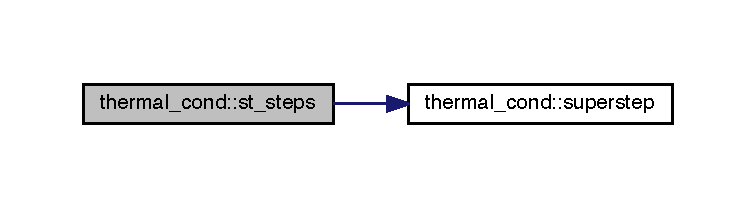
\includegraphics[width=348pt]{namespacethermal__cond_a4c74dc0fd6a165d0fea419b560943701_cgraph}
\end{center}
\end{figure}


\hypertarget{namespacethermal__cond_a782aaba01217281f2aa57dcc955fd294}{}\index{thermal\+\_\+cond@{thermal\+\_\+cond}!substep@{substep}}
\index{substep@{substep}!thermal\+\_\+cond@{thermal\+\_\+cond}}
\subsubsection[{substep}]{\setlength{\rightskip}{0pt plus 5cm}real function thermal\+\_\+cond\+::substep (
\begin{DoxyParamCaption}
\item[{integer, intent(in)}]{j, }
\item[{integer, intent(in)}]{N, }
\item[{real, intent(in)}]{nu}
\end{DoxyParamCaption}
)}\label{namespacethermal__cond_a782aaba01217281f2aa57dcc955fd294}
Returns the size of substep j of N 
\begin{DoxyParams}{Parameters}
{\em integer} & \mbox{[}in\mbox{]} j \+: index of current step \\
\hline
{\em integer} & \mbox{[}in\mbox{]} N \+: Total number of substeps \\
\hline
{\em real} & \mbox{[}in\mbox{]} nu \+: da\+M\+P\+I\+\_\+\+N\+Bg factor \\
\hline
\end{DoxyParams}


Definition at line 656 of file thermal\+\_\+cond.\+f90.

\hypertarget{namespacethermal__cond_a535cc1746914d413d4978aeda7b8fc06}{}\index{thermal\+\_\+cond@{thermal\+\_\+cond}!superstep@{superstep}}
\index{superstep@{superstep}!thermal\+\_\+cond@{thermal\+\_\+cond}}
\subsubsection[{superstep}]{\setlength{\rightskip}{0pt plus 5cm}real function thermal\+\_\+cond\+::superstep (
\begin{DoxyParamCaption}
\item[{integer}]{N, }
\item[{real, intent(in)}]{snu}
\end{DoxyParamCaption}
)}\label{namespacethermal__cond_a535cc1746914d413d4978aeda7b8fc06}
Returns the length of the superstep with N inner substeps 
\begin{DoxyParams}{Parameters}
{\em integer} & \mbox{[}in\mbox{]} N \+: Nunber of inner substeps \\
\hline
{\em real} & \mbox{[}in\mbox{]} snu \+: sqrt of da\+M\+P\+I\+\_\+\+N\+Bg factor \\
\hline
\end{DoxyParams}


Definition at line 635 of file thermal\+\_\+cond.\+f90.

\hypertarget{namespacethermal__cond_a55e65df0c700580f8af0a090063d2e32}{}\index{thermal\+\_\+cond@{thermal\+\_\+cond}!thermal\+\_\+bounds@{thermal\+\_\+bounds}}
\index{thermal\+\_\+bounds@{thermal\+\_\+bounds}!thermal\+\_\+cond@{thermal\+\_\+cond}}
\subsubsection[{thermal\+\_\+bounds}]{\setlength{\rightskip}{0pt plus 5cm}subroutine thermal\+\_\+cond\+::thermal\+\_\+bounds (
\begin{DoxyParamCaption}
{}
\end{DoxyParamCaption}
)}\label{namespacethermal__cond_a55e65df0c700580f8af0a090063d2e32}
Exchanges one layer of boundaries, only the equation that corresponds to the energy 

Definition at line 508 of file thermal\+\_\+cond.\+f90.

\hypertarget{namespacethermal__cond_a4b579df47b3bf4622a3ab51f57aa436b}{}\index{thermal\+\_\+cond@{thermal\+\_\+cond}!thermal\+\_\+conduction@{thermal\+\_\+conduction}}
\index{thermal\+\_\+conduction@{thermal\+\_\+conduction}!thermal\+\_\+cond@{thermal\+\_\+cond}}
\subsubsection[{thermal\+\_\+conduction}]{\setlength{\rightskip}{0pt plus 5cm}subroutine thermal\+\_\+cond\+::thermal\+\_\+conduction (
\begin{DoxyParamCaption}
{}
\end{DoxyParamCaption}
)}\label{namespacethermal__cond_a4b579df47b3bf4622a3ab51f57aa436b}
This routine adds the heat conduction, receives the hydro timestep in seconds, and assumes the primitives and Temp(i,j,k) arrays are updated 

Definition at line 700 of file thermal\+\_\+cond.\+f90.



Here is the call graph for this function\+:
% FIG 1



\chapter{File Documentation}
\hypertarget{mainpage_8h}{}\section{doc/mainpage.h File Reference}
\label{mainpage_8h}\index{doc/mainpage.\+h@{doc/mainpage.\+h}}


Webpage frontend.  



\hypertarget{boundaries_8f90}{}\section{/\+Users/esquivel/\+Desktop/\+Guacho-\/\+Working/src/boundaries.f90 File Reference}
\label{boundaries_8f90}\index{/\+Users/esquivel/\+Desktop/\+Guacho-\/\+Working/src/boundaries.\+f90@{/\+Users/esquivel/\+Desktop/\+Guacho-\/\+Working/src/boundaries.\+f90}}


Boundary conditions.  


\subsection*{Modules}
\begin{DoxyCompactItemize}
\item 
module \hyperlink{namespaceboundaries}{boundaries}
\begin{DoxyCompactList}\small\item\em Boundary conditions. \end{DoxyCompactList}\end{DoxyCompactItemize}
\subsection*{Functions/\+Subroutines}
\begin{DoxyCompactItemize}
\item 
subroutine \hyperlink{namespaceboundaries_a6292ba1e627b19087dc005cdc415213d}{boundaries\+::boundaryi} ()
\begin{DoxyCompactList}\small\item\em Boundary conditions for 1st order half timestep. \end{DoxyCompactList}\item 
subroutine \hyperlink{namespaceboundaries_acca5de134bd57d541d58574471fd8419}{boundaries\+::boundaryii} ()
\begin{DoxyCompactList}\small\item\em Boundary conditions for 2nd order half timestep. \end{DoxyCompactList}\end{DoxyCompactItemize}


\subsection{Detailed Description}
\begin{DoxyAuthor}{Author}
Alejandro Esquivel 
\end{DoxyAuthor}
\begin{DoxyDate}{Date}
2/\+Nov/2014 
\end{DoxyDate}

\hypertarget{chemistry_8f90}{}\section{/\+Users/esquivel/\+Desktop/\+Guacho-\/\+Working/src/chemistry.f90 File Reference}
\label{chemistry_8f90}\index{/\+Users/esquivel/\+Desktop/\+Guacho-\/\+Working/src/chemistry.\+f90@{/\+Users/esquivel/\+Desktop/\+Guacho-\/\+Working/src/chemistry.\+f90}}


chemistry module  


\subsection*{Modules}
\begin{DoxyCompactItemize}
\item 
module \hyperlink{namespacechemistry}{chemistry}
\begin{DoxyCompactList}\small\item\em chenistry module \end{DoxyCompactList}\end{DoxyCompactItemize}
\subsection*{Functions/\+Subroutines}
\begin{DoxyCompactItemize}
\item 
subroutine \hyperlink{namespacechemistry_a33dc05889bfc2d0361a4a3f95086f68c}{chemistry\+::update\+\_\+chem} ()
\begin{DoxyCompactList}\small\item\em Advances the chemistry network. \end{DoxyCompactList}\item 
subroutine \hyperlink{namespacechemistry_ab808252fa02b3bfb1ac29ed7b2f5122e}{chemistry\+::chemstep} (y, y0, T, deltt)
\begin{DoxyCompactList}\small\item\em Advances the chemistry network in one cell. \end{DoxyCompactList}\end{DoxyCompactItemize}


\subsection{Detailed Description}
\begin{DoxyAuthor}{Author}
A. Castellanos, A. Rodriguez, A. Raga and A. Esquivel 
\end{DoxyAuthor}
\begin{DoxyDate}{Date}
10/\+Mar/2016 
\end{DoxyDate}

\hypertarget{coldens_8f90}{}\section{src/coldens.f90 File Reference}
\label{coldens_8f90}\index{src/coldens.\+f90@{src/coldens.\+f90}}


Column density projection.  


\subsection*{Modules}
\begin{DoxyCompactItemize}
\item 
module \hyperlink{namespacecoldens__utilities}{coldens\+\_\+utilities}
\begin{DoxyCompactList}\small\item\em Column densirt projection. \end{DoxyCompactList}\end{DoxyCompactItemize}
\subsection*{Functions/\+Subroutines}
\begin{DoxyCompactItemize}
\item 
subroutine \hyperlink{namespacecoldens__utilities_a9fa20a511c2b17a33fdb8fc1b3bf55a2}{coldens\+\_\+utilities\+::init\+\_\+coldens} ()
\begin{DoxyCompactList}\small\item\em Initializes data. \end{DoxyCompactList}\item 
subroutine \hyperlink{namespacecoldens__utilities_a2dafe54f1edb888f313949f4f801e2d6}{coldens\+\_\+utilities\+::read\+\_\+data} (u, itprint, filepath)
\begin{DoxyCompactList}\small\item\em reads data from file \end{DoxyCompactList}\item 
subroutine \hyperlink{namespacecoldens__utilities_a7df7ce1cf8187ca5393dc35effa22020}{coldens\+\_\+utilities\+::getxyz} (i, j, k, x, y, z)
\begin{DoxyCompactList}\small\item\em gets position of a cell \end{DoxyCompactList}\item 
subroutine \hyperlink{namespacecoldens__utilities_af7f94bfb5ffee491708d3f221915abcf}{coldens\+\_\+utilities\+::rotation\+\_\+x} (theta, x, y, z, xn, yn, zn)
\begin{DoxyCompactList}\small\item\em Rotation around the X axis. \end{DoxyCompactList}\item 
subroutine \hyperlink{namespacecoldens__utilities_a989fb82adc69b6b1c00a2d2400c9854a}{coldens\+\_\+utilities\+::rotation\+\_\+y} (theta, x, y, z, xn, yn, zn)
\begin{DoxyCompactList}\small\item\em Rotation around the Y axis. \end{DoxyCompactList}\item 
subroutine \hyperlink{namespacecoldens__utilities_a062761acebb4d5a76b3706256a491687}{coldens\+\_\+utilities\+::rotation\+\_\+z} (theta, x, y, z, xn, yn, zn)
\begin{DoxyCompactList}\small\item\em Rotation around the Z axis. \end{DoxyCompactList}\item 
subroutine \hyperlink{namespacecoldens__utilities_af035b829538114f8b62f54365269bdab}{coldens\+\_\+utilities\+::fill\+\_\+map} (nxmap, nymap, u, map, dx\+T, dy\+T, theta\+\_\+x, theta\+\_\+y, theta\+\_\+z)
\begin{DoxyCompactList}\small\item\em Fill target map. \end{DoxyCompactList}\item 
subroutine \hyperlink{namespacecoldens__utilities_a78891c0c5736f8d50bf07d19757e7237}{coldens\+\_\+utilities\+::write\+\_\+map} (fileout, nxmap, nymap, map)
\begin{DoxyCompactList}\small\item\em Writes projection to file. \end{DoxyCompactList}\item 
program \hyperlink{coldens_8f90_afefbded5281bf1a352bcda7a729b23a6}{coldens}
\begin{DoxyCompactList}\small\item\em Computes the H-\/alpha emission. \end{DoxyCompactList}\end{DoxyCompactItemize}


\subsection{Detailed Description}
\begin{DoxyAuthor}{Author}
Alejandro Esquivel 
\end{DoxyAuthor}
\begin{DoxyDate}{Date}
2/\+Nov/2014 
\end{DoxyDate}


\subsection{Function/\+Subroutine Documentation}
\hypertarget{coldens_8f90_afefbded5281bf1a352bcda7a729b23a6}{}\index{coldens.\+f90@{coldens.\+f90}!coldens@{coldens}}
\index{coldens@{coldens}!coldens.\+f90@{coldens.\+f90}}
\subsubsection[{coldens}]{\setlength{\rightskip}{0pt plus 5cm}program coldens (
\begin{DoxyParamCaption}
{}
\end{DoxyParamCaption}
)}\label{coldens_8f90_afefbded5281bf1a352bcda7a729b23a6}
Computes the H-\/alpha apbsorption ~\newline
 It rotates the data along each of the coordinates axis by an amount $ \theta_x, \theta_y, \theta_z $, and projectcs the map along the the L\+O\+S, which is taken to be the Z axis 

Definition at line 370 of file coldens.\+f90.



Here is the call graph for this function\+:\nopagebreak
\begin{figure}[H]
\begin{center}
\leavevmode
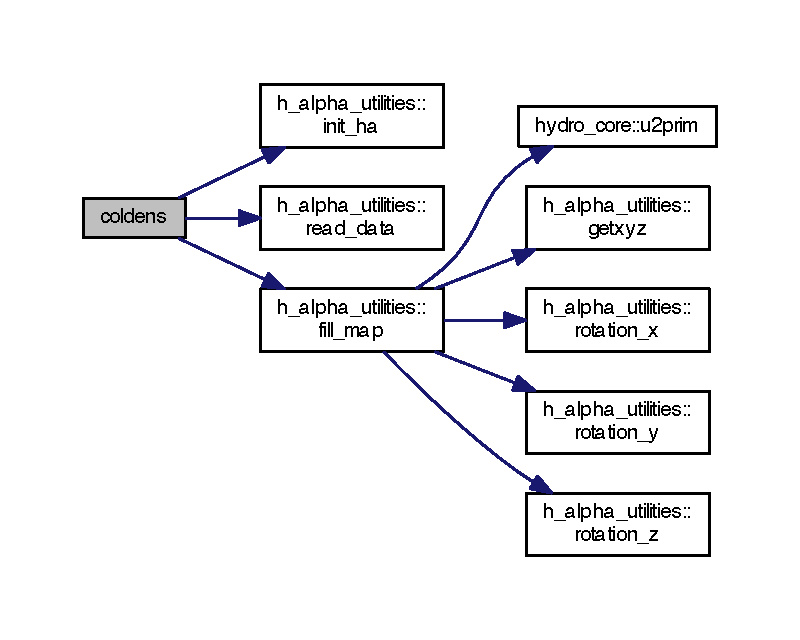
\includegraphics[width=350pt]{coldens_8f90_afefbded5281bf1a352bcda7a729b23a6_cgraph}
\end{center}
\end{figure}



\hypertarget{constants_8f90}{}\section{/\+Users/esquivel/\+Desktop/\+Guacho-\/\+Working/src/constants.f90 File Reference}
\label{constants_8f90}\index{/\+Users/esquivel/\+Desktop/\+Guacho-\/\+Working/src/constants.\+f90@{/\+Users/esquivel/\+Desktop/\+Guacho-\/\+Working/src/constants.\+f90}}


Constants module.  


\subsection*{Modules}
\begin{DoxyCompactItemize}
\item 
module \hyperlink{namespaceconstants}{constants}
\begin{DoxyCompactList}\small\item\em Module containing physical and asronomical constants. \end{DoxyCompactList}\end{DoxyCompactItemize}
\subsection*{Variables}
\begin{DoxyCompactItemize}
\item 
\hypertarget{namespaceconstants_a815ad954ef712211ed1b1fdb8be42487}{}real, parameter \hyperlink{namespaceconstants_a815ad954ef712211ed1b1fdb8be42487}{constants\+::pi} =acos(-\/1.)\label{namespaceconstants_a815ad954ef712211ed1b1fdb8be42487}

\begin{DoxyCompactList}\small\item\em $ \pi $ \end{DoxyCompactList}\item 
\hypertarget{namespaceconstants_aac258d92ad409a5ad7f8748101e932b0}{}real, parameter \hyperlink{namespaceconstants_aac258d92ad409a5ad7f8748101e932b0}{constants\+::amh} =1.\+66e-\/24\label{namespaceconstants_aac258d92ad409a5ad7f8748101e932b0}

\begin{DoxyCompactList}\small\item\em hydrogen mass \end{DoxyCompactList}\item 
\hypertarget{namespaceconstants_afc7b29a52df069e705256c11de562808}{}real, parameter \hyperlink{namespaceconstants_afc7b29a52df069e705256c11de562808}{constants\+::kb} =1.\+38e-\/16\label{namespaceconstants_afc7b29a52df069e705256c11de562808}

\begin{DoxyCompactList}\small\item\em Boltzmann constant (cgs) \end{DoxyCompactList}\item 
\hypertarget{namespaceconstants_aab4c0a2b0e8b8cda79e9d683b3e650f6}{}real, parameter \hyperlink{namespaceconstants_aab4c0a2b0e8b8cda79e9d683b3e650f6}{constants\+::rg} =8.\+3145e7\label{namespaceconstants_aab4c0a2b0e8b8cda79e9d683b3e650f6}

\begin{DoxyCompactList}\small\item\em Gas constant (cgs) \end{DoxyCompactList}\item 
\hypertarget{namespaceconstants_a1e2651b5b314d8b869a9a48b1063f126}{}real, parameter \hyperlink{namespaceconstants_a1e2651b5b314d8b869a9a48b1063f126}{constants\+::ggrav} =6.\+67259e-\/8\label{namespaceconstants_a1e2651b5b314d8b869a9a48b1063f126}

\begin{DoxyCompactList}\small\item\em Gravitational constant (cgs) \end{DoxyCompactList}\item 
\hypertarget{namespaceconstants_ac15de49d1114e2e8d78a3e77e2c0ebd0}{}real, parameter \hyperlink{namespaceconstants_ac15de49d1114e2e8d78a3e77e2c0ebd0}{constants\+::clight} =2.\+99\+E10\label{namespaceconstants_ac15de49d1114e2e8d78a3e77e2c0ebd0}

\begin{DoxyCompactList}\small\item\em speed of light in vacuum (cgs) \end{DoxyCompactList}\item 
\hypertarget{namespaceconstants_a47dcdcdf147127ab93252565436ce046}{}real, parameter \hyperlink{namespaceconstants_a47dcdcdf147127ab93252565436ce046}{constants\+::msun} =1.\+99\+E33\label{namespaceconstants_a47dcdcdf147127ab93252565436ce046}

\begin{DoxyCompactList}\small\item\em solar radius (cgs) \end{DoxyCompactList}\item 
\hypertarget{namespaceconstants_a86e80095a8a44315466905ab42ec2814}{}real, parameter \hyperlink{namespaceconstants_a86e80095a8a44315466905ab42ec2814}{constants\+::rsun} =6.\+955e10\label{namespaceconstants_a86e80095a8a44315466905ab42ec2814}

\begin{DoxyCompactList}\small\item\em solar mass (cgs) \end{DoxyCompactList}\item 
\hypertarget{namespaceconstants_a399e5e2bceae23d80dfe33489603dfa5}{}real, parameter \hyperlink{namespaceconstants_a399e5e2bceae23d80dfe33489603dfa5}{constants\+::mjup} =1.\+898\+E30\label{namespaceconstants_a399e5e2bceae23d80dfe33489603dfa5}

\begin{DoxyCompactList}\small\item\em Jupiter mass (cgs) \end{DoxyCompactList}\item 
\hypertarget{namespaceconstants_a4cbd85fb12d8faa8be8463982fa6fd29}{}real, parameter \hyperlink{namespaceconstants_a4cbd85fb12d8faa8be8463982fa6fd29}{constants\+::rjup} =7.\+1492\+E9\label{namespaceconstants_a4cbd85fb12d8faa8be8463982fa6fd29}

\begin{DoxyCompactList}\small\item\em Jupiter radius (cgs) \end{DoxyCompactList}\item 
\hypertarget{namespaceconstants_aba9a695c84a59f13c2d528a170a43b65}{}real, parameter \hyperlink{namespaceconstants_aba9a695c84a59f13c2d528a170a43b65}{constants\+::au} =1.\+496e13\label{namespaceconstants_aba9a695c84a59f13c2d528a170a43b65}

\begin{DoxyCompactList}\small\item\em 1\+A\+U in cm \end{DoxyCompactList}\item 
\hypertarget{namespaceconstants_aa5d9aea15e53a1abbc29e5f419b38601}{}real, parameter \hyperlink{namespaceconstants_aa5d9aea15e53a1abbc29e5f419b38601}{constants\+::pc} =3.\+0857\+E18\label{namespaceconstants_aa5d9aea15e53a1abbc29e5f419b38601}

\begin{DoxyCompactList}\small\item\em 1pc in cm \end{DoxyCompactList}\item 
\hypertarget{namespaceconstants_aee24dfdb51a8ed33a59bb80e98938718}{}real, parameter \hyperlink{namespaceconstants_aee24dfdb51a8ed33a59bb80e98938718}{constants\+::kpc} =3.\+0857\+E21\label{namespaceconstants_aee24dfdb51a8ed33a59bb80e98938718}

\begin{DoxyCompactList}\small\item\em 1\+Kpc in cm \end{DoxyCompactList}\item 
\hypertarget{namespaceconstants_a1c0cbdbdc4f321db2055f6cd61cdd3f4}{}real, parameter \hyperlink{namespaceconstants_a1c0cbdbdc4f321db2055f6cd61cdd3f4}{constants\+::hr} =3600.\label{namespaceconstants_a1c0cbdbdc4f321db2055f6cd61cdd3f4}

\begin{DoxyCompactList}\small\item\em 1hr in seconds \end{DoxyCompactList}\item 
\hypertarget{namespaceconstants_a9578082af66e4af5e4101e39b4abde29}{}real, parameter \hyperlink{namespaceconstants_a9578082af66e4af5e4101e39b4abde29}{constants\+::day} =86400.\label{namespaceconstants_a9578082af66e4af5e4101e39b4abde29}

\begin{DoxyCompactList}\small\item\em 1day in seconds \end{DoxyCompactList}\item 
\hypertarget{namespaceconstants_a1fd58880de7afc0479eb60d136bac8b2}{}real, parameter \hyperlink{namespaceconstants_a1fd58880de7afc0479eb60d136bac8b2}{constants\+::yr} =3.\+1536\+E7\label{namespaceconstants_a1fd58880de7afc0479eb60d136bac8b2}

\begin{DoxyCompactList}\small\item\em 1yr in seconds \end{DoxyCompactList}\item 
\hypertarget{namespaceconstants_af554c9cfbc1f3c74a8176265ea5370dd}{}real, parameter \hyperlink{namespaceconstants_af554c9cfbc1f3c74a8176265ea5370dd}{constants\+::myr} =3.\+1536\+E13\label{namespaceconstants_af554c9cfbc1f3c74a8176265ea5370dd}

\begin{DoxyCompactList}\small\item\em 1\+Myr in seconds \end{DoxyCompactList}\end{DoxyCompactItemize}


\subsection{Detailed Description}
\begin{DoxyAuthor}{Author}
Alejandro Esquivel 
\end{DoxyAuthor}
\begin{DoxyDate}{Date}
2/\+Nov/2014 
\end{DoxyDate}

\hypertarget{cooling__chi_8f90}{}\section{src/cooling\+\_\+chi.f90 File Reference}
\label{cooling__chi_8f90}\index{src/cooling\+\_\+chi.\+f90@{src/cooling\+\_\+chi.\+f90}}


Cooling module with C\+H\+I\+A\+N\+T\+I generated cooling curves.  


\subsection*{Modules}
\begin{DoxyCompactItemize}
\item 
module \hyperlink{namespacecooling__chi}{cooling\+\_\+chi}
\begin{DoxyCompactList}\small\item\em Cooling module with C\+H\+I\+A\+N\+T\+I generated cooling curves. \end{DoxyCompactList}\end{DoxyCompactItemize}
\subsection*{Functions/\+Subroutines}
\begin{DoxyCompactItemize}
\item 
subroutine \hyperlink{namespacecooling__chi_acdcfaea636dd68b666577d8daf434d35}{cooling\+\_\+chi\+::read\+\_\+table} ()
\begin{DoxyCompactList}\small\item\em Reads the cooling curve table. \end{DoxyCompactList}\item 
real(kind=8) function \hyperlink{namespacecooling__chi_a20c87eb43e4f324fa7d83fe9174fd767}{cooling\+\_\+chi\+::coolchi} (T)
\begin{DoxyCompactList}\small\item\em Returns the cooling coefficient interpolating the table. \end{DoxyCompactList}\item 
subroutine \hyperlink{namespacecooling__chi_a16ac452561e4a332a960a3ea7304f103}{cooling\+\_\+chi\+::coolingchi} (dt)
\begin{DoxyCompactList}\small\item\em High level wrapper to apply cooling with C\+H\+I\+A\+N\+T\+I tables. \end{DoxyCompactList}\end{DoxyCompactItemize}
\subsection*{Variables}
\begin{DoxyCompactItemize}
\item 
\hypertarget{namespacecooling__chi_a37baf8c1757edb98fcaa8b62587d7b2f}{}real(kind=8), dimension(2, 41) {\bfseries cooling\+\_\+chi\+::cooltab}\label{namespacecooling__chi_a37baf8c1757edb98fcaa8b62587d7b2f}

\end{DoxyCompactItemize}


\subsection{Detailed Description}
\begin{DoxyAuthor}{Author}
Alejandro Esquivel 
\end{DoxyAuthor}
\begin{DoxyDate}{Date}
2/\+Nov/2014 
\end{DoxyDate}

\hypertarget{cooling__dmc_8f90}{}\section{/\+Users/esquivel/\+Desktop/\+Guacho-\/\+Working/src/cooling\+\_\+dmc.f90 File Reference}
\label{cooling__dmc_8f90}\index{/\+Users/esquivel/\+Desktop/\+Guacho-\/\+Working/src/cooling\+\_\+dmc.\+f90@{/\+Users/esquivel/\+Desktop/\+Guacho-\/\+Working/src/cooling\+\_\+dmc.\+f90}}


Cooling module with Dlgarno Mac Cray coronal cooling curve.  


\subsection*{Modules}
\begin{DoxyCompactItemize}
\item 
module \hyperlink{namespacecooling__dmc}{cooling\+\_\+dmc}
\begin{DoxyCompactList}\small\item\em Cooling module with Dalgarno Mc\+Cray coronal cooling curve. \end{DoxyCompactList}\end{DoxyCompactItemize}
\subsection*{Functions/\+Subroutines}
\begin{DoxyCompactItemize}
\item 
subroutine \hyperlink{namespacecooling__dmc_a7874b4f8a76399e87e0a22aecd088cf8}{cooling\+\_\+dmc\+::read\+\_\+table} ()
\begin{DoxyCompactList}\small\item\em Reads the cooling curve table. \end{DoxyCompactList}\item 
real(kind=8) function \hyperlink{namespacecooling__dmc_af987bbf144f596d57b154427bbb82ae5}{cooling\+\_\+dmc\+::cooldmc} (T)
\begin{DoxyCompactList}\small\item\em Returns the cooling coefficient interpolating the table. \end{DoxyCompactList}\item 
subroutine \hyperlink{namespacecooling__dmc_a7af28062f0cd20c4bb0d86c895f4a8d6}{cooling\+\_\+dmc\+::coolingdmc} ()
\begin{DoxyCompactList}\small\item\em High level wrapper to apply cooling with D\+M\+C table. \end{DoxyCompactList}\end{DoxyCompactItemize}
\subsection*{Variables}
\begin{DoxyCompactItemize}
\item 
\hypertarget{namespacecooling__dmc_aa692bc7125c6e889f3cf993f9f48f9d3}{}real(kind=8), dimension(2, 41) {\bfseries cooling\+\_\+dmc\+::cooltab}\label{namespacecooling__dmc_aa692bc7125c6e889f3cf993f9f48f9d3}

\end{DoxyCompactItemize}


\subsection{Detailed Description}
\begin{DoxyAuthor}{Author}
Alejandro Esquivel 
\end{DoxyAuthor}
\begin{DoxyDate}{Date}
2/\+Nov/2014 
\end{DoxyDate}

\hypertarget{cooling__h_8f90}{}\section{/\+Users/esquivel/\+Desktop/\+Guacho-\/\+Working/src/cooling\+\_\+h.f90 File Reference}
\label{cooling__h_8f90}\index{/\+Users/esquivel/\+Desktop/\+Guacho-\/\+Working/src/cooling\+\_\+h.\+f90@{/\+Users/esquivel/\+Desktop/\+Guacho-\/\+Working/src/cooling\+\_\+h.\+f90}}


Cooling with hydrogen rate parametrized cooling.  


\subsection*{Modules}
\begin{DoxyCompactItemize}
\item 
module \hyperlink{namespacecooling__h}{cooling\+\_\+h}
\begin{DoxyCompactList}\small\item\em Cooling with parametrized cooling and H rate equation. \end{DoxyCompactList}\end{DoxyCompactItemize}
\subsection*{Functions/\+Subroutines}
\begin{DoxyCompactItemize}
\item 
subroutine \hyperlink{namespacecooling__h_aee85faa3b36e05a8efb05c1588f34ef2}{cooling\+\_\+h\+::coolingh} ()
\begin{DoxyCompactList}\small\item\em High level wrapper to apply cooling. \end{DoxyCompactList}\item 
real(kind=8) function \hyperlink{namespacecooling__h_a09de30645cebf531a647b5f53ae143b2}{cooling\+\_\+h\+::alpha} (T)
\begin{DoxyCompactList}\small\item\em calculates the recombination rate (case B) \end{DoxyCompactList}\item 
real(kind=8) function \hyperlink{namespacecooling__h_a5454f21ef468add797c58753a1e0c773}{cooling\+\_\+h\+::alpha1} (T)
\begin{DoxyCompactList}\small\item\em calculates the recombination rate to level 1 \end{DoxyCompactList}\item 
real(kind=8) function \hyperlink{namespacecooling__h_ad5f1352f8925ccb1b352d6e749465a92}{cooling\+\_\+h\+::colf} (T)
\begin{DoxyCompactList}\small\item\em calculates the collisional ionization rate \end{DoxyCompactList}\item 
real(kind=8) function \hyperlink{namespacecooling__h_a2a2de25572bd515eae9441391e0ed0f8}{cooling\+\_\+h\+::betah} (T)
\begin{DoxyCompactList}\small\item\em beta\+H(\+T) \end{DoxyCompactList}\item 
real(kind=8) function \hyperlink{namespacecooling__h_a92cfd14c9b02e853eb33d22857fabeed}{cooling\+\_\+h\+::aloss} (X1, X2, D\+T, D\+E\+N, D\+H0, T\+E0)
\begin{DoxyCompactList}\small\item\em Non equilibrium cooling. \end{DoxyCompactList}\item 
subroutine \hyperlink{namespacecooling__h_aef95dbca5e7aef78d66a225cc217c982}{cooling\+\_\+h\+::atomic} (dt, uu, tau, radphi)
\begin{DoxyCompactList}\small\item\em Updates the ionization fraction and applpies cooling. \end{DoxyCompactList}\end{DoxyCompactItemize}


\subsection{Detailed Description}
\begin{DoxyAuthor}{Author}
Alejandro Esquivel 
\end{DoxyAuthor}
\begin{DoxyDate}{Date}
2/\+Nov/2014 
\end{DoxyDate}

\hypertarget{difrad_8f90}{}\section{/\+Users/esquivel/\+Desktop/\+Guacho-\/\+Working/src/difrad.f90 File Reference}
\label{difrad_8f90}\index{/\+Users/esquivel/\+Desktop/\+Guacho-\/\+Working/src/difrad.\+f90@{/\+Users/esquivel/\+Desktop/\+Guacho-\/\+Working/src/difrad.\+f90}}


Diffuse radiation module.  


\subsection*{Modules}
\begin{DoxyCompactItemize}
\item 
module \hyperlink{namespacedifrad}{difrad}
\begin{DoxyCompactList}\small\item\em Ray tracing Radiative Trasnport. \end{DoxyCompactList}\end{DoxyCompactItemize}
\subsection*{Functions/\+Subroutines}
\begin{DoxyCompactItemize}
\item 
subroutine \hyperlink{namespacedifrad_a9bce19025195159710828548c95282dc}{difrad\+::init\+\_\+rand} ()
\begin{DoxyCompactList}\small\item\em initializes random number generation \end{DoxyCompactList}\item 
subroutine \hyperlink{namespacedifrad_a1ccb144621689571d836f2f76c5fabae}{difrad\+::emdiff} (emax)
\begin{DoxyCompactList}\small\item\em calculates the diffuse fotoionization emissivity \end{DoxyCompactList}\item 
subroutine \hyperlink{namespacedifrad_ac7efbacd89420f5c298f7fb666ba14f9}{difrad\+::random\+\_\+versor} (xd, yd, zd)
\begin{DoxyCompactList}\small\item\em returns the 3 components of a random versor \end{DoxyCompactList}\item 
subroutine \hyperlink{namespacedifrad_a180fbbe2c9b0639cc33dd6ef57a61ec4}{difrad\+::starsource} (srad, x0, y0, z0, x, y, z, xd, yd, zd)
\begin{DoxyCompactList}\small\item\em Place photon packets at a \char`\"{}star\char`\"{} surface. \end{DoxyCompactList}\item 
subroutine \hyperlink{namespacedifrad_a39291c8aa2927c69ef6ca60f78c9b103}{difrad\+::photons} (xl0, yl0, zl0, xd, yd, zd, f)
\begin{DoxyCompactList}\small\item\em Photon trajectories. \end{DoxyCompactList}\item 
subroutine \hyperlink{namespacedifrad_afe6e9d2182e755ae483aeaa2c91f2710}{difrad\+::radbounds} ()
\begin{DoxyCompactList}\small\item\em follows the rays across M\+P\+I boundaries \end{DoxyCompactList}\item 
subroutine \hyperlink{namespacedifrad_a17151a5334db41fd14315d454e883b8e}{difrad\+::progress} (j, tot)
\begin{DoxyCompactList}\small\item\em Progress bar. \end{DoxyCompactList}\item 
subroutine \hyperlink{namespacedifrad_aeec1cd3dae50e6946aadb42abef934ec}{difrad\+::diffuse\+\_\+rad} ()
\begin{DoxyCompactList}\small\item\em Diffuse radiation driver. \end{DoxyCompactList}\end{DoxyCompactItemize}
\subsection*{Variables}
\begin{DoxyCompactItemize}
\item 
\hypertarget{namespacedifrad_a0062472e34b740c2c1cb5084d3284056}{}real, parameter \hyperlink{namespacedifrad_a0062472e34b740c2c1cb5084d3284056}{difrad\+::a0} =6.\+3e-\/18\label{namespacedifrad_a0062472e34b740c2c1cb5084d3284056}

\begin{DoxyCompactList}\small\item\em Fotoionization cross section. \end{DoxyCompactList}\item 
\hypertarget{namespacedifrad_aac6943b42d4dede95a3296bdc29c629a}{}integer, parameter \hyperlink{namespacedifrad_aac6943b42d4dede95a3296bdc29c629a}{difrad\+::nrays} =1000000\label{namespacedifrad_aac6943b42d4dede95a3296bdc29c629a}

\begin{DoxyCompactList}\small\item\em Number of rays. \end{DoxyCompactList}\item 
\hypertarget{namespacedifrad_ab532f1879434284f63aa97c79c305236}{}real, dimension(\+:,\+:,\+:), allocatable \hyperlink{namespacedifrad_ab532f1879434284f63aa97c79c305236}{difrad\+::ph}\label{namespacedifrad_ab532f1879434284f63aa97c79c305236}

\begin{DoxyCompactList}\small\item\em Photoionizing rate. \end{DoxyCompactList}\item 
\hypertarget{namespacedifrad_a7d908916fd1e050b9c5ba48771186d5b}{}real, dimension(\+:,\+:,\+:), allocatable \hyperlink{namespacedifrad_a7d908916fd1e050b9c5ba48771186d5b}{difrad\+::em}\label{namespacedifrad_a7d908916fd1e050b9c5ba48771186d5b}

\begin{DoxyCompactList}\small\item\em Photoionizing emissivity. \end{DoxyCompactList}\item 
\hypertarget{namespacedifrad_a3d6a043ec876c626f11238b6260a036a}{}real, dimension(\+:,\+:,\+:), allocatable \hyperlink{namespacedifrad_a3d6a043ec876c626f11238b6260a036a}{difrad\+::photl}\label{namespacedifrad_a3d6a043ec876c626f11238b6260a036a}

\begin{DoxyCompactList}\small\item\em Auxiliary buffer for M\+P\+I. \end{DoxyCompactList}\item 
\hypertarget{namespacedifrad_adf49e979d01582a3c0032f9bde3c4555}{}real, dimension(\+:,\+:,\+:), allocatable \hyperlink{namespacedifrad_adf49e979d01582a3c0032f9bde3c4555}{difrad\+::photr}\label{namespacedifrad_adf49e979d01582a3c0032f9bde3c4555}

\begin{DoxyCompactList}\small\item\em Auxiliary buffer for M\+P\+I. \end{DoxyCompactList}\item 
\hypertarget{namespacedifrad_a65e54816218f7e0acae4ffeaaf9523f6}{}real, dimension(\+:,\+:,\+:), allocatable \hyperlink{namespacedifrad_a65e54816218f7e0acae4ffeaaf9523f6}{difrad\+::photb}\label{namespacedifrad_a65e54816218f7e0acae4ffeaaf9523f6}

\begin{DoxyCompactList}\small\item\em Auxiliary buffer for M\+P\+I. \end{DoxyCompactList}\item 
\hypertarget{namespacedifrad_a28892e6d6f67cbcb8b65e79132cf959b}{}real, dimension(\+:,\+:,\+:), allocatable \hyperlink{namespacedifrad_a28892e6d6f67cbcb8b65e79132cf959b}{difrad\+::phott}\label{namespacedifrad_a28892e6d6f67cbcb8b65e79132cf959b}

\begin{DoxyCompactList}\small\item\em Auxiliary buffer for M\+P\+I. \end{DoxyCompactList}\item 
\hypertarget{namespacedifrad_a73a81002fda23212ff6d9d8b6d161f32}{}real, dimension(\+:,\+:,\+:), allocatable \hyperlink{namespacedifrad_a73a81002fda23212ff6d9d8b6d161f32}{difrad\+::photo}\label{namespacedifrad_a73a81002fda23212ff6d9d8b6d161f32}

\begin{DoxyCompactList}\small\item\em Auxiliary buffer for M\+P\+I. \end{DoxyCompactList}\item 
\hypertarget{namespacedifrad_afa84bdf37b43d72b3e3e3b3c6291807e}{}real, dimension(\+:,\+:,\+:), allocatable \hyperlink{namespacedifrad_afa84bdf37b43d72b3e3e3b3c6291807e}{difrad\+::photi}\label{namespacedifrad_afa84bdf37b43d72b3e3e3b3c6291807e}

\begin{DoxyCompactList}\small\item\em Auxiliary buffer for M\+P\+I. \end{DoxyCompactList}\item 
\hypertarget{namespacedifrad_a1d5243b742ea3504f1b6b09132417333}{}integer, dimension(6) \hyperlink{namespacedifrad_a1d5243b742ea3504f1b6b09132417333}{difrad\+::buffersize}\label{namespacedifrad_a1d5243b742ea3504f1b6b09132417333}

\begin{DoxyCompactList}\small\item\em Auxiliary buffer for M\+P\+I. \end{DoxyCompactList}\end{DoxyCompactItemize}


\subsection{Detailed Description}
\begin{DoxyAuthor}{Author}
Alejandro Esquivel 
\end{DoxyAuthor}
\begin{DoxyDate}{Date}
2/\+Nov/2014 
\end{DoxyDate}

\hypertarget{globals_8f90}{}\section{/\+Users/esquivel/\+Desktop/\+Guacho-\/\+Working/src/globals.f90 File Reference}
\label{globals_8f90}\index{/\+Users/esquivel/\+Desktop/\+Guacho-\/\+Working/src/globals.\+f90@{/\+Users/esquivel/\+Desktop/\+Guacho-\/\+Working/src/globals.\+f90}}


Global variables.  


\subsection*{Modules}
\begin{DoxyCompactItemize}
\item 
module \hyperlink{namespaceglobals}{globals}
\begin{DoxyCompactList}\small\item\em Module containing global variables. \end{DoxyCompactList}\end{DoxyCompactItemize}
\subsection*{Variables}
\begin{DoxyCompactItemize}
\item 
\hypertarget{namespaceglobals_ae6519b751f8ef608c2074e27024335b7}{}real, dimension(\+:,\+:,\+:,\+:), allocatable \hyperlink{namespaceglobals_ae6519b751f8ef608c2074e27024335b7}{globals\+::u}\label{namespaceglobals_ae6519b751f8ef608c2074e27024335b7}

\begin{DoxyCompactList}\small\item\em conserved varibles \end{DoxyCompactList}\item 
\hypertarget{namespaceglobals_a127abb71c460a346ae47d10d86c22cc9}{}real, dimension(\+:,\+:,\+:,\+:), allocatable \hyperlink{namespaceglobals_a127abb71c460a346ae47d10d86c22cc9}{globals\+::up}\label{namespaceglobals_a127abb71c460a346ae47d10d86c22cc9}

\begin{DoxyCompactList}\small\item\em conserved varibles after 1/2 timestep \end{DoxyCompactList}\item 
\hypertarget{namespaceglobals_a149bece4e7407071629f69a8c7deb03a}{}real, dimension(\+:,\+:,\+:,\+:), allocatable \hyperlink{namespaceglobals_a149bece4e7407071629f69a8c7deb03a}{globals\+::primit}\label{namespaceglobals_a149bece4e7407071629f69a8c7deb03a}

\begin{DoxyCompactList}\small\item\em primitive varibles \end{DoxyCompactList}\item 
\hypertarget{namespaceglobals_a5fb85172ca54e822fdb8c522da890717}{}real, dimension(\+:,\+:,\+:,\+:), allocatable \hyperlink{namespaceglobals_a5fb85172ca54e822fdb8c522da890717}{globals\+::f}\label{namespaceglobals_a5fb85172ca54e822fdb8c522da890717}

\begin{DoxyCompactList}\small\item\em X fluxes. \end{DoxyCompactList}\item 
\hypertarget{namespaceglobals_a0124c44fda4a3092edd2789f79dec648}{}real, dimension(\+:,\+:,\+:,\+:), allocatable \hyperlink{namespaceglobals_a0124c44fda4a3092edd2789f79dec648}{globals\+::g}\label{namespaceglobals_a0124c44fda4a3092edd2789f79dec648}

\begin{DoxyCompactList}\small\item\em Y fluxes. \end{DoxyCompactList}\item 
\hypertarget{namespaceglobals_af6262d058b86075848725c846e7cc9cc}{}real, dimension(\+:,\+:,\+:,\+:), allocatable \hyperlink{namespaceglobals_af6262d058b86075848725c846e7cc9cc}{globals\+::h}\label{namespaceglobals_af6262d058b86075848725c846e7cc9cc}

\begin{DoxyCompactList}\small\item\em Z fluxes. \end{DoxyCompactList}\item 
\hypertarget{namespaceglobals_aafee650389fdf595e41e37cb340155ae}{}real \hyperlink{namespaceglobals_aafee650389fdf595e41e37cb340155ae}{globals\+::dx}\label{namespaceglobals_aafee650389fdf595e41e37cb340155ae}

\begin{DoxyCompactList}\small\item\em grid spacing in X \end{DoxyCompactList}\item 
\hypertarget{namespaceglobals_a9b12323045a0672fe06f9b7091cd3e7a}{}real \hyperlink{namespaceglobals_a9b12323045a0672fe06f9b7091cd3e7a}{globals\+::dy}\label{namespaceglobals_a9b12323045a0672fe06f9b7091cd3e7a}

\begin{DoxyCompactList}\small\item\em grid spacing in Y \end{DoxyCompactList}\item 
\hypertarget{namespaceglobals_a81293f145f1af171eb88b6feced78c95}{}real \hyperlink{namespaceglobals_a81293f145f1af171eb88b6feced78c95}{globals\+::dz}\label{namespaceglobals_a81293f145f1af171eb88b6feced78c95}

\begin{DoxyCompactList}\small\item\em grid spacing in Z \end{DoxyCompactList}\item 
\hypertarget{namespaceglobals_a8d38eca539ad2b24a66616e42b79ac4c}{}integer, dimension(0\+:2) \hyperlink{namespaceglobals_a8d38eca539ad2b24a66616e42b79ac4c}{globals\+::coords}\label{namespaceglobals_a8d38eca539ad2b24a66616e42b79ac4c}

\begin{DoxyCompactList}\small\item\em position of neighboring M\+P\+I blocks \end{DoxyCompactList}\item 
\hypertarget{namespaceglobals_aba9a16c1b0ed3e52dce83157476d099c}{}integer \hyperlink{namespaceglobals_aba9a16c1b0ed3e52dce83157476d099c}{globals\+::left}\label{namespaceglobals_aba9a16c1b0ed3e52dce83157476d099c}

\begin{DoxyCompactList}\small\item\em M\+P\+I neighbor in the -\/x direction. \end{DoxyCompactList}\item 
\hypertarget{namespaceglobals_a0b27e5c90473860434fc5dd58a255111}{}integer \hyperlink{namespaceglobals_a0b27e5c90473860434fc5dd58a255111}{globals\+::right}\label{namespaceglobals_a0b27e5c90473860434fc5dd58a255111}

\begin{DoxyCompactList}\small\item\em M\+P\+I neighbor in the +x direction. \end{DoxyCompactList}\item 
\hypertarget{namespaceglobals_add36bccef8d272ff40330a62d0307580}{}integer \hyperlink{namespaceglobals_add36bccef8d272ff40330a62d0307580}{globals\+::top}\label{namespaceglobals_add36bccef8d272ff40330a62d0307580}

\begin{DoxyCompactList}\small\item\em M\+P\+I neighbor in the -\/y direction. \end{DoxyCompactList}\item 
\hypertarget{namespaceglobals_a3188a89193263f9f063099801321d525}{}integer \hyperlink{namespaceglobals_a3188a89193263f9f063099801321d525}{globals\+::bottom}\label{namespaceglobals_a3188a89193263f9f063099801321d525}

\begin{DoxyCompactList}\small\item\em M\+P\+I neighbor in the +y direction. \end{DoxyCompactList}\item 
\hypertarget{namespaceglobals_ac3375149d8b96b3b5470274034850ecc}{}integer \hyperlink{namespaceglobals_ac3375149d8b96b3b5470274034850ecc}{globals\+::out}\label{namespaceglobals_ac3375149d8b96b3b5470274034850ecc}

\begin{DoxyCompactList}\small\item\em M\+P\+I neighbor in the -\/z direction. \end{DoxyCompactList}\item 
\hypertarget{namespaceglobals_a6a2cc973507c2f9ea75f44a9f976d659}{}integer \hyperlink{namespaceglobals_a6a2cc973507c2f9ea75f44a9f976d659}{globals\+::in}\label{namespaceglobals_a6a2cc973507c2f9ea75f44a9f976d659}

\begin{DoxyCompactList}\small\item\em M\+P\+I neighbor in the +z direction. \end{DoxyCompactList}\item 
\hypertarget{namespaceglobals_a93f283242b146b3ef8b53fd1b1ad7bac}{}integer \hyperlink{namespaceglobals_a93f283242b146b3ef8b53fd1b1ad7bac}{globals\+::rank}\label{namespaceglobals_a93f283242b146b3ef8b53fd1b1ad7bac}

\begin{DoxyCompactList}\small\item\em M\+P\+I rank. \end{DoxyCompactList}\item 
\hypertarget{namespaceglobals_a4bc8f1b5670efd802d57dce2c385b6d9}{}integer \hyperlink{namespaceglobals_a4bc8f1b5670efd802d57dce2c385b6d9}{globals\+::comm3d}\label{namespaceglobals_a4bc8f1b5670efd802d57dce2c385b6d9}

\begin{DoxyCompactList}\small\item\em Cartessian M\+P\+I comunicator. \end{DoxyCompactList}\item 
\hypertarget{namespaceglobals_acc5c9a03b08561f9eeb530eb65221dbb}{}real \hyperlink{namespaceglobals_acc5c9a03b08561f9eeb530eb65221dbb}{globals\+::time}\label{namespaceglobals_acc5c9a03b08561f9eeb530eb65221dbb}

\begin{DoxyCompactList}\small\item\em Current time. \end{DoxyCompactList}\item 
\hypertarget{namespaceglobals_a1599fd11dcd5dfa9104003de3a2d03e5}{}real \hyperlink{namespaceglobals_a1599fd11dcd5dfa9104003de3a2d03e5}{globals\+::dt\+\_\+cfl}\label{namespaceglobals_a1599fd11dcd5dfa9104003de3a2d03e5}

\begin{DoxyCompactList}\small\item\em Current C\+F\+L \$ t\$. \end{DoxyCompactList}\item 
\hypertarget{namespaceglobals_a6966cf52ad4f442a7fe69efa6d5c0bee}{}integer \hyperlink{namespaceglobals_a6966cf52ad4f442a7fe69efa6d5c0bee}{globals\+::currentiteration}\label{namespaceglobals_a6966cf52ad4f442a7fe69efa6d5c0bee}

\begin{DoxyCompactList}\small\item\em Current iteration. \end{DoxyCompactList}\item 
\hypertarget{namespaceglobals_a6942102ba8bd15a3350901de0b99bafa}{}real, dimension(\+:,\+:,\+:), allocatable \hyperlink{namespaceglobals_a6942102ba8bd15a3350901de0b99bafa}{globals\+::temp}\label{namespaceglobals_a6942102ba8bd15a3350901de0b99bafa}

\begin{DoxyCompactList}\small\item\em Temperature array \mbox{[}K\mbox{]}. \end{DoxyCompactList}\end{DoxyCompactItemize}


\subsection{Detailed Description}
\begin{DoxyAuthor}{Author}
Alejandro Esquivel 
\end{DoxyAuthor}
\begin{DoxyDate}{Date}
2/\+Nov/2014 
\end{DoxyDate}

\hypertarget{h__alpha__proj_8f90}{}\section{src/h\+\_\+alpha\+\_\+proj.f90 File Reference}
\label{h__alpha__proj_8f90}\index{src/h\+\_\+alpha\+\_\+proj.\+f90@{src/h\+\_\+alpha\+\_\+proj.\+f90}}


H alpha projection.  


\subsection*{Modules}
\begin{DoxyCompactItemize}
\item 
module \hyperlink{namespaceh__alpha__utilities}{h\+\_\+alpha\+\_\+utilities}
\begin{DoxyCompactList}\small\item\em H alpha projection. \end{DoxyCompactList}\end{DoxyCompactItemize}
\subsection*{Functions/\+Subroutines}
\begin{DoxyCompactItemize}
\item 
subroutine \hyperlink{namespaceh__alpha__utilities_a8bb4ef22ad133f8d3f75cf1a26e14035}{h\+\_\+alpha\+\_\+utilities\+::init\+\_\+ha} ()
\begin{DoxyCompactList}\small\item\em Initializes data. \end{DoxyCompactList}\item 
subroutine \hyperlink{namespaceh__alpha__utilities_a5549bf9fd812d02d9189d27f380c01c0}{h\+\_\+alpha\+\_\+utilities\+::read\+\_\+data} (u, itprint, filepath)
\begin{DoxyCompactList}\small\item\em reads data from file \end{DoxyCompactList}\item 
subroutine \hyperlink{namespaceh__alpha__utilities_af48cd3c223c292170bc1f90da256f537}{h\+\_\+alpha\+\_\+utilities\+::getxyz} (i, j, k, x, y, z)
\begin{DoxyCompactList}\small\item\em gets position of a cell \end{DoxyCompactList}\item 
subroutine \hyperlink{namespaceh__alpha__utilities_a65ad5d15c1265e31f4d191ebf771e669}{h\+\_\+alpha\+\_\+utilities\+::rotation\+\_\+x} (theta, x, y, z, xn, yn, zn)
\begin{DoxyCompactList}\small\item\em Rotation around the X axis. \end{DoxyCompactList}\item 
subroutine \hyperlink{namespaceh__alpha__utilities_ab643f1bac838912c58b25923b5de40ca}{h\+\_\+alpha\+\_\+utilities\+::rotation\+\_\+y} (theta, x, y, z, xn, yn, zn)
\begin{DoxyCompactList}\small\item\em Rotation around the Y axis. \end{DoxyCompactList}\item 
subroutine \hyperlink{namespaceh__alpha__utilities_acaf25f2c0ad80c5d7e2f451f58522a49}{h\+\_\+alpha\+\_\+utilities\+::rotation\+\_\+z} (theta, x, y, z, xn, yn, zn)
\begin{DoxyCompactList}\small\item\em Rotation around the Z axis. \end{DoxyCompactList}\item 
subroutine \hyperlink{namespaceh__alpha__utilities_aafc5cae88b562d0bd2d039cae21ed35a}{h\+\_\+alpha\+\_\+utilities\+::fill\+\_\+map} (nxmap, nymap, u, map, dx\+T, dy\+T, theta\+\_\+x, theta\+\_\+y, theta\+\_\+z)
\begin{DoxyCompactList}\small\item\em Fill target map. \end{DoxyCompactList}\item 
subroutine \hyperlink{namespaceh__alpha__utilities_aa2b2b3783ef4b30d178412ea44671047}{h\+\_\+alpha\+\_\+utilities\+::write\+\_\+ha} (fileout, nxmap, nymap, map)
\begin{DoxyCompactList}\small\item\em Writes projection to file. \end{DoxyCompactList}\item 
subroutine \hyperlink{namespaceh__alpha__utilities_a1cf6b2b4be1a68c792b3cb07b5629af6}{h\+\_\+alpha\+\_\+utilities\+::write\+\_\+rg} (fileout, nxmap, nymap, map)
\begin{DoxyCompactList}\small\item\em Writes projection to file in rg format. \end{DoxyCompactList}\item 
program \hyperlink{h__alpha__proj_8f90_ae4326230e4f19e2e66573778f131e5c3}{h\+\_\+alpha\+\_\+proj}
\begin{DoxyCompactList}\small\item\em Computes the H-\/alpha emission. \end{DoxyCompactList}\end{DoxyCompactItemize}


\subsection{Detailed Description}
\begin{DoxyAuthor}{Author}
Alejandro Esquivel 
\end{DoxyAuthor}
\begin{DoxyDate}{Date}
2/\+Nov/2014 
\end{DoxyDate}


\subsection{Function/\+Subroutine Documentation}
\hypertarget{h__alpha__proj_8f90_ae4326230e4f19e2e66573778f131e5c3}{}\index{h\+\_\+alpha\+\_\+proj.\+f90@{h\+\_\+alpha\+\_\+proj.\+f90}!h\+\_\+alpha\+\_\+proj@{h\+\_\+alpha\+\_\+proj}}
\index{h\+\_\+alpha\+\_\+proj@{h\+\_\+alpha\+\_\+proj}!h\+\_\+alpha\+\_\+proj.\+f90@{h\+\_\+alpha\+\_\+proj.\+f90}}
\subsubsection[{h\+\_\+alpha\+\_\+proj}]{\setlength{\rightskip}{0pt plus 5cm}program h\+\_\+alpha\+\_\+proj (
\begin{DoxyParamCaption}
{}
\end{DoxyParamCaption}
)}\label{h__alpha__proj_8f90_ae4326230e4f19e2e66573778f131e5c3}
Computes the H-\/alpha apbsorption ~\newline
 It rotates the data along each of the coordinates axis by an amount $ \theta_x, \theta_y, \theta_z $, and projectcs the map along the the L\+O\+S, which is taken to be the Z axis 

Definition at line 428 of file h\+\_\+alpha\+\_\+proj.\+f90.



Here is the call graph for this function\+:\nopagebreak
\begin{figure}[H]
\begin{center}
\leavevmode
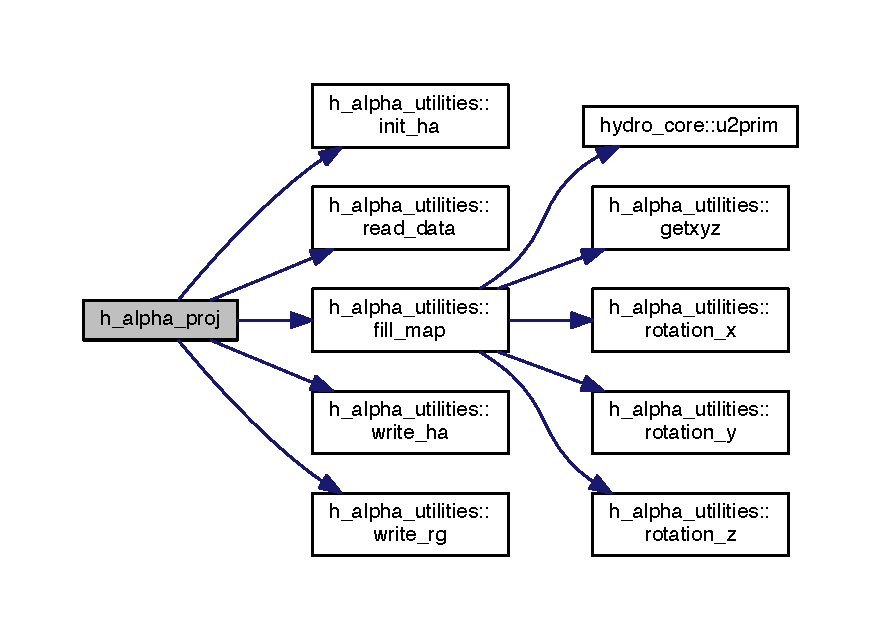
\includegraphics[width=350pt]{h__alpha__proj_8f90_ae4326230e4f19e2e66573778f131e5c3_cgraph}
\end{center}
\end{figure}



\hypertarget{hll_8f90}{}\section{/\+Users/esquivel/\+Desktop/\+Guacho-\/\+Working/src/hll.f90 File Reference}
\label{hll_8f90}\index{/\+Users/esquivel/\+Desktop/\+Guacho-\/\+Working/src/hll.\+f90@{/\+Users/esquivel/\+Desktop/\+Guacho-\/\+Working/src/hll.\+f90}}


H\+L\+L approximate Riemann solver module.  


\subsection*{Modules}
\begin{DoxyCompactItemize}
\item 
module \hyperlink{namespacehll}{hll}
\begin{DoxyCompactList}\small\item\em H\+L\+L approximate Riemann solver module. \end{DoxyCompactList}\end{DoxyCompactItemize}
\subsection*{Functions/\+Subroutines}
\begin{DoxyCompactItemize}
\item 
subroutine \hyperlink{namespacehll_aa67c7db7e17f7dedf7286320baeda1dd}{hll\+::prim2fhll} (priml, primr, ff)
\begin{DoxyCompactList}\small\item\em Solves the Riemann problem at the interface P\+L,P\+R using the H\+L\+L solver. \end{DoxyCompactList}\item 
subroutine \hyperlink{namespacehll_a27386fb5bcf705be5e8c2650484966c6}{hll\+::hllfluxes} (choice)
\begin{DoxyCompactList}\small\item\em Calculates H\+L\+L fluxes from the primitive variables on all the domain. \end{DoxyCompactList}\end{DoxyCompactItemize}


\subsection{Detailed Description}
\begin{DoxyAuthor}{Author}
Alejandro Esquivel 
\end{DoxyAuthor}
\begin{DoxyDate}{Date}
2/\+Nov/2014 
\end{DoxyDate}

\hypertarget{hllc_8f90}{}\section{src/hllc.f90 File Reference}
\label{hllc_8f90}\index{src/hllc.\+f90@{src/hllc.\+f90}}


H\+L\+L\+C approximate Riemann solver module.  


\subsection*{Modules}
\begin{DoxyCompactItemize}
\item 
module \hyperlink{namespacehllc}{hllc}
\begin{DoxyCompactList}\small\item\em H\+L\+L\+C approximate Riemann solver module. \end{DoxyCompactList}\end{DoxyCompactItemize}
\subsection*{Functions/\+Subroutines}
\begin{DoxyCompactItemize}
\item 
subroutine \hyperlink{namespacehllc_a25f1f218ed55fbda8b6311baa3ff6f80}{hllc\+::prim2fhllc} (priml, primr, ff)
\begin{DoxyCompactList}\small\item\em Solves the Riemann problem at the interface P\+L,P\+R using the H\+L\+L\+C solver. \end{DoxyCompactList}\item 
subroutine \hyperlink{namespacehllc_a702fd4ba2d419a6ac6d21a9bc25ba230}{hllc\+::hllcfluxes} (choice)
\begin{DoxyCompactList}\small\item\em Calculates H\+L\+L\+C fluxes from the primitive variables on all the domain. \end{DoxyCompactList}\end{DoxyCompactItemize}


\subsection{Detailed Description}
\begin{DoxyAuthor}{Author}
Alejandro Esquivel 
\end{DoxyAuthor}
\begin{DoxyDate}{Date}
2/\+Nov/2014 
\end{DoxyDate}

\hypertarget{hlld_8f90}{}\section{src/hlld.f90 File Reference}
\label{hlld_8f90}\index{src/hlld.\+f90@{src/hlld.\+f90}}


H\+L\+L\+D approximate Riemann solver module.  


\subsection*{Modules}
\begin{DoxyCompactItemize}
\item 
module \hyperlink{namespacehlld}{hlld}
\begin{DoxyCompactList}\small\item\em H\+L\+L\+D approximate Riemann solver module. \end{DoxyCompactList}\end{DoxyCompactItemize}
\subsection*{Functions/\+Subroutines}
\begin{DoxyCompactItemize}
\item 
subroutine \hyperlink{namespacehlld_adb0dbc5abe3e062f2ee4e333c6794bc8}{hlld\+::prim2fhlld} (priml, primr, ff)
\begin{DoxyCompactList}\small\item\em Solves the Riemann problem at the interface P\+L,P\+R using the H\+L\+L\+D solver. \end{DoxyCompactList}\item 
subroutine \hyperlink{namespacehlld_a2640822e1b56d5b174f6293c26d75e22}{hlld\+::hlldfluxes} (choice)
\begin{DoxyCompactList}\small\item\em Calculates H\+L\+L\+D fluxes from the primitive variables on all the domain. \end{DoxyCompactList}\end{DoxyCompactItemize}


\subsection{Detailed Description}
\begin{DoxyAuthor}{Author}
C. Villarreal D\textquotesingle{}Angelo, A. Esquivel, M. Schneiter 
\end{DoxyAuthor}
\begin{DoxyDate}{Date}
2/\+Nov/2014 
\end{DoxyDate}

\hypertarget{hlle_8f90}{}\section{/\+Users/esquivel/\+Desktop/\+Guacho-\/\+Working/src/hlle.f90 File Reference}
\label{hlle_8f90}\index{/\+Users/esquivel/\+Desktop/\+Guacho-\/\+Working/src/hlle.\+f90@{/\+Users/esquivel/\+Desktop/\+Guacho-\/\+Working/src/hlle.\+f90}}


H\+L\+L\+E approximate Riemann solver module.  


\subsection*{Modules}
\begin{DoxyCompactItemize}
\item 
module \hyperlink{namespacehlle}{hlle}
\begin{DoxyCompactList}\small\item\em H\+L\+L\+E approximate Riemann solver module. \end{DoxyCompactList}\end{DoxyCompactItemize}
\subsection*{Functions/\+Subroutines}
\begin{DoxyCompactItemize}
\item 
subroutine \hyperlink{namespacehlle_a5646b0259c574b5e8dd3754a493d358d}{hlle\+::prim2fhlle} (priml, primr, ff)
\begin{DoxyCompactList}\small\item\em Solves the Riemann problem at the interface P\+L,P\+R using the H\+L\+L\+E solver. \end{DoxyCompactList}\item 
subroutine \hyperlink{namespacehlle_a03540214994c25ce07877114dd37b641}{hlle\+::hllefluxes} (choice)
\begin{DoxyCompactList}\small\item\em Calculates H\+L\+L\+E fluxes from the primitive variables on all the domain. \end{DoxyCompactList}\end{DoxyCompactItemize}


\subsection{Detailed Description}
\begin{DoxyAuthor}{Author}
C. Villarreal D\textquotesingle{}Angelo, A. Esquivel, M. Schneiter 
\end{DoxyAuthor}
\begin{DoxyDate}{Date}
2/\+Nov/2014 
\end{DoxyDate}

\hypertarget{hydro__core_8f90}{}\section{src/hydro\+\_\+core.f90 File Reference}
\label{hydro__core_8f90}\index{src/hydro\+\_\+core.\+f90@{src/hydro\+\_\+core.\+f90}}


Hydrodynamical and Magnetohidrodynamocal bacic module.  


\subsection*{Modules}
\begin{DoxyCompactItemize}
\item 
module \hyperlink{namespacehydro__core}{hydro\+\_\+core}
\begin{DoxyCompactList}\small\item\em Basic hydro (and M\+H\+D) subroutines utilities. \end{DoxyCompactList}\end{DoxyCompactItemize}
\subsection*{Functions/\+Subroutines}
\begin{DoxyCompactItemize}
\item 
subroutine \hyperlink{namespacehydro__core_a360e3d64343b30d94d270cfebc5b4eb3}{hydro\+\_\+core\+::u2prim} (uu, prim, T)
\begin{DoxyCompactList}\small\item\em Computes the primitive variables and temperature from conserved variables on a single cell. \end{DoxyCompactList}\item 
subroutine \hyperlink{namespacehydro__core_a991a14316cc93864150071b30fd9c772}{hydro\+\_\+core\+::calcprim} (u, primit)
\begin{DoxyCompactList}\small\item\em Updated the primitives, using the conserved variables in the entire domain. \end{DoxyCompactList}\item 
subroutine \hyperlink{namespacehydro__core_a98cafc8f97d7a1b3f8050b8e442194c3}{hydro\+\_\+core\+::prim2u} (prim, uu)
\begin{DoxyCompactList}\small\item\em Computes the conserved conserved variables from the primitives in a single cell. \end{DoxyCompactList}\item 
subroutine \hyperlink{namespacehydro__core_a725c2c598f080ea420f4043dbda3f996}{hydro\+\_\+core\+::prim2f} (prim, ff)
\begin{DoxyCompactList}\small\item\em Computes the Euler Fluxes in one cell. \end{DoxyCompactList}\item 
subroutine \hyperlink{namespacehydro__core_a64856096f7a7b7f65be1154d31916c2d}{hydro\+\_\+core\+::swapy} (var, neq)
\begin{DoxyCompactList}\small\item\em Swaps the x and y components in a cell. \end{DoxyCompactList}\item 
subroutine \hyperlink{namespacehydro__core_ae4216bc7908e7665f0565aa8c885c821}{hydro\+\_\+core\+::swapz} (var, neq)
\begin{DoxyCompactList}\small\item\em Swaps the x and z components in a cell. \end{DoxyCompactList}\item 
subroutine \hyperlink{namespacehydro__core_a27cb7ddb40cc0226e0139bd9eba42dfa}{hydro\+\_\+core\+::csound} (p, d, cs)
\begin{DoxyCompactList}\small\item\em Computes the sound speed. \end{DoxyCompactList}\item 
subroutine \hyperlink{namespacehydro__core_ab2655b81626d4d95cb003112248e928a}{hydro\+\_\+core\+::cfast} (p, d, bx, by, bz, cfx, cfy, cfz)
\begin{DoxyCompactList}\small\item\em Computes the fast magnetosonic speeds in the 3 coordinates. \end{DoxyCompactList}\item 
subroutine \hyperlink{namespacehydro__core_abd089f71325e32997703c1420db62aa8}{hydro\+\_\+core\+::cfastx} (prim, cf\+X)
\begin{DoxyCompactList}\small\item\em Computes the fast magnetosonic speed in the x direction. \end{DoxyCompactList}\item 
subroutine \hyperlink{namespacehydro__core_a0b0402ba5c94d738eb020f79783f8d53}{hydro\+\_\+core\+::get\+\_\+timestep} (dt)
\begin{DoxyCompactList}\small\item\em Otains the timestep allowed by the C\+F\+L condition in the entire. \end{DoxyCompactList}\item 
subroutine \hyperlink{namespacehydro__core_ada63ca89d1a40cfd1a62db0ddfdbda80}{hydro\+\_\+core\+::limiter} (P\+L\+L, P\+L, P\+R, P\+R\+R, neq)
\begin{DoxyCompactList}\small\item\em Performs a linear reconstruction of the primitive variables. \end{DoxyCompactList}\item 
\hypertarget{hydro__core_8f90_a6d27fe4138b4de2f5bb7448e9eafc4ee}{}real function {\bfseries average} (a, b)\label{hydro__core_8f90_a6d27fe4138b4de2f5bb7448e9eafc4ee}

\end{DoxyCompactItemize}


\subsection{Detailed Description}
\begin{DoxyAuthor}{Author}
Alejandro Esquivel 
\end{DoxyAuthor}
\begin{DoxyDate}{Date}
2/\+Nov/2014 
\end{DoxyDate}

\hypertarget{hydro__solver_8f90}{}\section{src/hydro\+\_\+solver.f90 File Reference}
\label{hydro__solver_8f90}\index{src/hydro\+\_\+solver.\+f90@{src/hydro\+\_\+solver.\+f90}}


Hydrodynamical and Magnetohidrodynamocal solver module.  


\subsection*{Modules}
\begin{DoxyCompactItemize}
\item 
module \hyperlink{namespacehydro__solver}{hydro\+\_\+solver}
\begin{DoxyCompactList}\small\item\em Advances the simulation one timestep. \end{DoxyCompactList}\end{DoxyCompactItemize}
\subsection*{Functions/\+Subroutines}
\begin{DoxyCompactItemize}
\item 
subroutine \hyperlink{namespacehydro__solver_a88127baf969063d6d9a31845fa7c1835}{hydro\+\_\+solver\+::viscosity} ()
\begin{DoxyCompactList}\small\item\em Adds artificial viscosity to the conserved variables. \end{DoxyCompactList}\item 
subroutine \hyperlink{namespacehydro__solver_ac34a166e9ddd81f20f2b271138458a1a}{hydro\+\_\+solver\+::step} (dt)
\begin{DoxyCompactList}\small\item\em Upwind timestep. \end{DoxyCompactList}\item 
subroutine \hyperlink{namespacehydro__solver_aca1a384e66d388e79ca981c0c84680a0}{hydro\+\_\+solver\+::tstep} (time, dt)
\begin{DoxyCompactList}\small\item\em High level wrapper to advancce the simulation. \end{DoxyCompactList}\end{DoxyCompactItemize}


\subsection{Detailed Description}
\begin{DoxyAuthor}{Author}
Alejandro Esquivel 
\end{DoxyAuthor}
\begin{DoxyDate}{Date}
2/\+Nov/2014 
\end{DoxyDate}

\hypertarget{init_8f90}{}\section{/\+Users/esquivel/\+Desktop/\+Guacho-\/\+Working/src/init.f90 File Reference}
\label{init_8f90}\index{/\+Users/esquivel/\+Desktop/\+Guacho-\/\+Working/src/init.\+f90@{/\+Users/esquivel/\+Desktop/\+Guacho-\/\+Working/src/init.\+f90}}


Guacho-\/3\+D initialization module.  


\subsection*{Modules}
\begin{DoxyCompactItemize}
\item 
module \hyperlink{namespaceinit}{init}
\begin{DoxyCompactList}\small\item\em Guacho-\/3\+D initialization. \end{DoxyCompactList}\end{DoxyCompactItemize}
\subsection*{Functions/\+Subroutines}
\begin{DoxyCompactItemize}
\item 
subroutine \hyperlink{namespaceinit_a60b4d8ee577d59490c7d351b73253a99}{init\+::initmain} (tprint, itprint)
\begin{DoxyCompactList}\small\item\em Main initialization routine. \end{DoxyCompactList}\item 
subroutine \hyperlink{namespaceinit_ab5415b25da1a9e732d3f557f4d6008b9}{init\+::initflow} (itprint)
\begin{DoxyCompactList}\small\item\em Initializes the conserved variables, in the globals module. \end{DoxyCompactList}\end{DoxyCompactItemize}


\subsection{Detailed Description}
\begin{DoxyAuthor}{Author}
Alejandro Esquivel 
\end{DoxyAuthor}
\begin{DoxyDate}{Date}
2/\+Nov/2014 
\end{DoxyDate}

\hypertarget{linear__system_8f90}{}\section{/\+Users/esquivel/\+Desktop/\+Guacho-\/\+Working/src/linear\+\_\+system.f90 File Reference}
\label{linear__system_8f90}\index{/\+Users/esquivel/\+Desktop/\+Guacho-\/\+Working/src/linear\+\_\+system.\+f90@{/\+Users/esquivel/\+Desktop/\+Guacho-\/\+Working/src/linear\+\_\+system.\+f90}}


linear system inversion module  


\subsection*{Modules}
\begin{DoxyCompactItemize}
\item 
module \hyperlink{namespacelinear__system}{linear\+\_\+system}
\begin{DoxyCompactList}\small\item\em linear system inversion module \end{DoxyCompactList}\end{DoxyCompactItemize}
\subsection*{Functions/\+Subroutines}
\begin{DoxyCompactItemize}
\item 
subroutine \hyperlink{namespacelinear__system_ad77fb788295266bcc818f72d6677bf9d}{linear\+\_\+system\+::ludcmp} (a, n, indx, d)
\begin{DoxyCompactList}\small\item\em L\+U decomposition. \end{DoxyCompactList}\item 
subroutine \hyperlink{namespacelinear__system_acdd63cedefa6077e4100904703d6b82d}{linear\+\_\+system\+::lubksb} (a, n, indx, b)
\begin{DoxyCompactList}\small\item\em Solves a set of linear equations. \end{DoxyCompactList}\item 
subroutine \hyperlink{namespacelinear__system_a51e9428c30e00182fa86755204de7762}{linear\+\_\+system\+::linsys} (a, b, n)
\begin{DoxyCompactList}\small\item\em Driver to solves a set of linear equations. \end{DoxyCompactList}\end{DoxyCompactItemize}


\subsection{Detailed Description}
\begin{DoxyAuthor}{Author}
A. Castellanos, A. Rodriguez, A. Raga and A. Esquivel 
\end{DoxyAuthor}
\begin{DoxyDate}{Date}
10/\+Mar/2016 
\end{DoxyDate}

\hypertarget{lyman__alpha__tau_8f90}{}\section{/\+Users/esquivel/\+Desktop/\+Guacho-\/\+Working/src/lyman\+\_\+alpha\+\_\+tau.f90 File Reference}
\label{lyman__alpha__tau_8f90}\index{/\+Users/esquivel/\+Desktop/\+Guacho-\/\+Working/src/lyman\+\_\+alpha\+\_\+tau.\+f90@{/\+Users/esquivel/\+Desktop/\+Guacho-\/\+Working/src/lyman\+\_\+alpha\+\_\+tau.\+f90}}


Lyman\+\_\+alpha\+\_\+utilities.  


\subsection*{Modules}
\begin{DoxyCompactItemize}
\item 
module \hyperlink{namespacelyman__alpha__utilities}{lyman\+\_\+alpha\+\_\+utilities}
\begin{DoxyCompactList}\small\item\em Lyman\+\_\+alpha\+\_\+utilities. \end{DoxyCompactList}\end{DoxyCompactItemize}
\subsection*{Functions/\+Subroutines}
\begin{DoxyCompactItemize}
\item 
subroutine \hyperlink{namespacelyman__alpha__utilities_a5f97eeffb7ea030271481514d7072efb}{lyman\+\_\+alpha\+\_\+utilities\+::init\+\_\+la} ()
\begin{DoxyCompactList}\small\item\em Initializes data. \end{DoxyCompactList}\item 
subroutine \hyperlink{namespacelyman__alpha__utilities_a75d86f06c6da27d0754752c23c50b54a}{lyman\+\_\+alpha\+\_\+utilities\+::read\+\_\+data} (u, itprint, filepath)
\begin{DoxyCompactList}\small\item\em reads data from file \end{DoxyCompactList}\item 
subroutine \hyperlink{namespacelyman__alpha__utilities_abdefc59ee98b1526aa3116c0e8f21d98}{lyman\+\_\+alpha\+\_\+utilities\+::getxyz} (i, j, k, x, y, z)
\begin{DoxyCompactList}\small\item\em gets position of a cell \end{DoxyCompactList}\item 
subroutine \hyperlink{namespacelyman__alpha__utilities_afaddcbb27f079d4300ce631609bbb80d}{lyman\+\_\+alpha\+\_\+utilities\+::rotation\+\_\+x} (theta, x, y, z, xn, yn, zn)
\begin{DoxyCompactList}\small\item\em Rotation around the X axis. \end{DoxyCompactList}\item 
subroutine \hyperlink{namespacelyman__alpha__utilities_ae865cec09dd956ff966316caf8ac0c9a}{lyman\+\_\+alpha\+\_\+utilities\+::rotation\+\_\+y} (theta, x, y, z, xn, yn, zn)
\begin{DoxyCompactList}\small\item\em Rotation around the Y axis. \end{DoxyCompactList}\item 
subroutine \hyperlink{namespacelyman__alpha__utilities_a2c97c4405186edcb70d2e37bbe7306da}{lyman\+\_\+alpha\+\_\+utilities\+::rotation\+\_\+z} (theta, x, y, z, xn, yn, zn)
\begin{DoxyCompactList}\small\item\em Rotation around the Z axis. \end{DoxyCompactList}\item 
subroutine \hyperlink{namespacelyman__alpha__utilities_a7ca5810d29123f1c5c6fd3170f5f5bf3}{lyman\+\_\+alpha\+\_\+utilities\+::fill\+\_\+map} (nxmap, nymap, nvmap, vmin, vmax, u, map, dx\+T, dy\+T, theta\+\_\+x, theta\+\_\+y, theta\+\_\+z)
\begin{DoxyCompactList}\small\item\em Fill target map. \end{DoxyCompactList}\item 
subroutine \hyperlink{namespacelyman__alpha__utilities_afdab7ea06bb95956c43102154651cfd1}{lyman\+\_\+alpha\+\_\+utilities\+::write\+\_\+la} (itprint, filepath, nxmap, nymap, nvmap, map)
\begin{DoxyCompactList}\small\item\em Writes projection to file. \end{DoxyCompactList}\item 
subroutine \hyperlink{namespacelyman__alpha__utilities_a826e6fe44f66513e5a47f2b968e1d0b8}{lyman\+\_\+alpha\+\_\+utilities\+::phigauss} (T, vzn, vmin, vmax, nvmap, profile)
\begin{DoxyCompactList}\small\item\em This routine computes a gaussian line profile. \end{DoxyCompactList}\item 
program \hyperlink{lyman__alpha__tau_8f90_ac17b5fa88f45d76c5707da8a09262fe7}{lyman\+\_\+alpha\+\_\+tau}
\begin{DoxyCompactList}\small\item\em Computes the Ly-\/alpha apbsorption. \end{DoxyCompactList}\end{DoxyCompactItemize}


\subsection{Detailed Description}
\begin{DoxyAuthor}{Author}
Alejandro Esquivel 
\end{DoxyAuthor}
\begin{DoxyDate}{Date}
2/\+Nov/2014 
\end{DoxyDate}


\subsection{Function/\+Subroutine Documentation}
\hypertarget{lyman__alpha__tau_8f90_ac17b5fa88f45d76c5707da8a09262fe7}{}\index{lyman\+\_\+alpha\+\_\+tau.\+f90@{lyman\+\_\+alpha\+\_\+tau.\+f90}!lyman\+\_\+alpha\+\_\+tau@{lyman\+\_\+alpha\+\_\+tau}}
\index{lyman\+\_\+alpha\+\_\+tau@{lyman\+\_\+alpha\+\_\+tau}!lyman\+\_\+alpha\+\_\+tau.\+f90@{lyman\+\_\+alpha\+\_\+tau.\+f90}}
\subsubsection[{lyman\+\_\+alpha\+\_\+tau}]{\setlength{\rightskip}{0pt plus 5cm}program lyman\+\_\+alpha\+\_\+tau (
\begin{DoxyParamCaption}
{}
\end{DoxyParamCaption}
)}\label{lyman__alpha__tau_8f90_ac17b5fa88f45d76c5707da8a09262fe7}
Computes the Ly-\/alpha apbsorption ~\newline
 It rotates the data along each of the coordinates axis by an amount $ \theta_x, \theta_y, \theta_z $, and the L\+O\+S is along the Z axis 

Definition at line 419 of file lyman\+\_\+alpha\+\_\+tau.\+f90.



Here is the call graph for this function\+:
% FIG 0



\hypertarget{main_8f90}{}\section{/\+Users/esquivel/\+Desktop/\+Guacho-\/\+Working/src/main.f90 File Reference}
\label{main_8f90}\index{/\+Users/esquivel/\+Desktop/\+Guacho-\/\+Working/src/main.\+f90@{/\+Users/esquivel/\+Desktop/\+Guacho-\/\+Working/src/main.\+f90}}


Guacho-\/3\+D main program.  


\subsection*{Functions/\+Subroutines}
\begin{DoxyCompactItemize}
\item 
\hypertarget{main_8f90_a685bddead5d9dcd4492c9cf9c60614a5}{}program \hyperlink{main_8f90_a685bddead5d9dcd4492c9cf9c60614a5}{guacho}\label{main_8f90_a685bddead5d9dcd4492c9cf9c60614a5}

\begin{DoxyCompactList}\small\item\em Guacho-\/3\+D Main Program This is the main program unit of the Guacho-\/3\+D code. ~\newline
 The code itegrates Euler equations in three dimensions, the choice of the integration method is set in the makefile. ~\newline
 The flow (conserved) variables are taken to be\+: ~\newline
 ieq= ~\newline
 1 \+: rho (total) ~\newline
 2 \+: rho u ~\newline
 3 \+: rho v ~\newline
 4 \+: rho w ~\newline
 5 \+: Internal energy (thermal+kinetic) ~\newline
 6 \+: bx (optional, if M\+H\+D or P\+M\+H\+D) ~\newline
 7 \+: by (optional, if M\+H\+D or P\+M\+H\+D) ~\newline
 8 \+: bz (optional, if M\+H\+D or P\+M\+H\+D) ~\newline
 additional variables advected into the flow, e.\+g.\+: ~\newline
 9 (6)\+: n\+\_\+\+H\+I ~\newline
 10 (7)\+: n\+\_\+\+H\+I\+I ~\newline
 11 (8)\+: n\+\_\+\+He\+I ~\newline
 12 (9)\+: n\+\_\+\+He\+I\+I ~\newline
 13 (10)\+: n\+\_\+\+He\+I\+I\+I ~\newline
 14 (11)\+: rho$\ast$zbar ~\newline
 15 (12)\+: ne ~\newline
 This can be changed bu the user according to cooling function for instance. \end{DoxyCompactList}\end{DoxyCompactItemize}


\subsection{Detailed Description}
\begin{DoxyAuthor}{Author}
Alejandro Esquivel 
\end{DoxyAuthor}
\begin{DoxyDate}{Date}
2/\+Nov/2014 
\end{DoxyDate}

\hypertarget{_out___b_i_n___module_8f90}{}\section{/\+Users/esquivel/\+Desktop/\+Guacho-\/\+Working/src/\+Out\+\_\+\+B\+I\+N\+\_\+\+Module.f90 File Reference}
\label{_out___b_i_n___module_8f90}\index{/\+Users/esquivel/\+Desktop/\+Guacho-\/\+Working/src/\+Out\+\_\+\+B\+I\+N\+\_\+\+Module.\+f90@{/\+Users/esquivel/\+Desktop/\+Guacho-\/\+Working/src/\+Out\+\_\+\+B\+I\+N\+\_\+\+Module.\+f90}}


Output in B\+I\+N Format.  


\subsection*{Modules}
\begin{DoxyCompactItemize}
\item 
module \hyperlink{namespaceout__bin__module}{out\+\_\+bin\+\_\+module}
\begin{DoxyCompactList}\small\item\em Output in B\+I\+N format. \end{DoxyCompactList}\end{DoxyCompactItemize}
\subsection*{Functions/\+Subroutines}
\begin{DoxyCompactItemize}
\item 
subroutine \hyperlink{namespaceout__bin__module_a6e5fb4bb1cc6f0a15ce591a3b1014d8d}{out\+\_\+bin\+\_\+module\+::write\+\_\+header} (unit, neq\+\_\+out, nghost\+\_\+out)
\begin{DoxyCompactList}\small\item\em Writes header. \end{DoxyCompactList}\item 
subroutine \hyperlink{namespaceout__bin__module_ac5772f05ffdd0227d2fc17e27beb0f59}{out\+\_\+bin\+\_\+module\+::write\+\_\+bin} (itprint)
\begin{DoxyCompactList}\small\item\em Writes Data, one file per processor. \end{DoxyCompactList}\end{DoxyCompactItemize}


\subsection{Detailed Description}
\begin{DoxyAuthor}{Author}
Alejandro Esquivel 
\end{DoxyAuthor}
\begin{DoxyDate}{Date}
2/\+Nov/2014 
\end{DoxyDate}

\hypertarget{_out___silo___module_8f90}{}\section{src/\+Out\+\_\+\+Silo\+\_\+\+Module.f90 File Reference}
\label{_out___silo___module_8f90}\index{src/\+Out\+\_\+\+Silo\+\_\+\+Module.\+f90@{src/\+Out\+\_\+\+Silo\+\_\+\+Module.\+f90}}


Output in Silo Format.  


\subsection*{Modules}
\begin{DoxyCompactItemize}
\item 
module \hyperlink{namespaceout__silo__module}{out\+\_\+silo\+\_\+module}
\begin{DoxyCompactList}\small\item\em Output in Silo (+\+H\+D\+F5) Format. \end{DoxyCompactList}\end{DoxyCompactItemize}
\subsection*{Functions/\+Subroutines}
\begin{DoxyCompactItemize}
\item 
subroutine \hyperlink{namespaceout__silo__module_acfa5a749647a6a7c95e48e3ad58e4139}{out\+\_\+silo\+\_\+module\+::writeblocks} (itprint)
\begin{DoxyCompactList}\small\item\em Writes Data, one file per processor. \end{DoxyCompactList}\item 
subroutine \hyperlink{namespaceout__silo__module_aa984d6044bf34559a87a9020c4a07c3a}{out\+\_\+silo\+\_\+module\+::writemaster} (itprint)
\begin{DoxyCompactList}\small\item\em Writes the Master File. \end{DoxyCompactList}\item 
subroutine \hyperlink{namespaceout__silo__module_a65763f848b9b5da2a20d8b55f53f8515}{out\+\_\+silo\+\_\+module\+::outputsilo} (itprint)
\begin{DoxyCompactList}\small\item\em Upper level wrapper. \end{DoxyCompactList}\end{DoxyCompactItemize}


\subsection{Detailed Description}
\begin{DoxyAuthor}{Author}
Alejandro Esquivel 
\end{DoxyAuthor}
\begin{DoxyDate}{Date}
2/\+Nov/2014 
\end{DoxyDate}

\hypertarget{_out___v_t_k___module_8f90}{}\section{/\+Users/esquivel/\+Desktop/\+Guacho-\/\+Working/src/\+Out\+\_\+\+V\+T\+K\+\_\+\+Module.f90 File Reference}
\label{_out___v_t_k___module_8f90}\index{/\+Users/esquivel/\+Desktop/\+Guacho-\/\+Working/src/\+Out\+\_\+\+V\+T\+K\+\_\+\+Module.\+f90@{/\+Users/esquivel/\+Desktop/\+Guacho-\/\+Working/src/\+Out\+\_\+\+V\+T\+K\+\_\+\+Module.\+f90}}


Output in V\+T\+K Format.  


\subsection*{Modules}
\begin{DoxyCompactItemize}
\item 
module \hyperlink{namespaceout__vtk__module}{out\+\_\+vtk\+\_\+module}
\begin{DoxyCompactList}\small\item\em Output in V\+T\+K format. \end{DoxyCompactList}\end{DoxyCompactItemize}
\subsection*{Functions/\+Subroutines}
\begin{DoxyCompactItemize}
\item 
subroutine \hyperlink{namespaceout__vtk__module_ac34f91e1b74dd533461d7ead905bf937}{out\+\_\+vtk\+\_\+module\+::write\+\_\+vtk} (itprint)
\begin{DoxyCompactList}\small\item\em Writes Data, one file per processor. \end{DoxyCompactList}\end{DoxyCompactItemize}


\subsection{Detailed Description}
\begin{DoxyAuthor}{Author}
Alejandro Esquivel 
\end{DoxyAuthor}
\begin{DoxyDate}{Date}
2/\+Nov/2014 
\end{DoxyDate}

\hypertarget{output_8f90}{}\section{src/output.f90 File Reference}
\label{output_8f90}\index{src/output.\+f90@{src/output.\+f90}}


Writes Output.  


\subsection*{Modules}
\begin{DoxyCompactItemize}
\item 
module \hyperlink{namespaceoutput}{output}
\begin{DoxyCompactList}\small\item\em Writes output. \end{DoxyCompactList}\end{DoxyCompactItemize}
\subsection*{Functions/\+Subroutines}
\begin{DoxyCompactItemize}
\item 
subroutine \hyperlink{namespaceoutput_a9a6f65196f6b514f504929c9e1f7582f}{output\+::write\+\_\+output} (itprint)
\begin{DoxyCompactList}\small\item\em Writes output. \end{DoxyCompactList}\end{DoxyCompactItemize}


\subsection{Detailed Description}
\begin{DoxyAuthor}{Author}
Alejandro Esquivel 
\end{DoxyAuthor}
\begin{DoxyDate}{Date}
2/\+Nov/2014 
\end{DoxyDate}

\hypertarget{sources_8f90}{}\section{src/sources.f90 File Reference}
\label{sources_8f90}\index{src/sources.\+f90@{src/sources.\+f90}}


Adds source terms.  


\subsection*{Modules}
\begin{DoxyCompactItemize}
\item 
module \hyperlink{namespacesources}{sources}
\begin{DoxyCompactList}\small\item\em Adds source terms. \end{DoxyCompactList}\end{DoxyCompactItemize}
\subsection*{Functions/\+Subroutines}
\begin{DoxyCompactItemize}
\item 
subroutine \hyperlink{namespacesources_a378a8116ae16db2efa853343f88156d3}{sources\+::getpos} (i, j, k, x, y, z, r)
\begin{DoxyCompactList}\small\item\em Gets position in the grid. \end{DoxyCompactList}\item 
subroutine \hyperlink{namespacesources_aef9f6ca4bc770f0e768dbbba91b67415}{sources\+::grav\+\_\+source} (xc, yc, zc, pp, s)
\begin{DoxyCompactList}\small\item\em Gravity due to point sources. \end{DoxyCompactList}\item 
subroutine \hyperlink{namespacesources_a36b548c9c578b74c5f439ffaec7d3a9a}{sources\+::radpress\+\_\+source} (i, j, k, xc, yc, zc, rc, pp, s)
\begin{DoxyCompactList}\small\item\em Radiation pressure force. \end{DoxyCompactList}\item 
subroutine \hyperlink{namespacesources_a0478795277b4f25ec62d8e3e1f06611e}{sources\+::divergence\+\_\+b} (i, j, k, d)
\begin{DoxyCompactList}\small\item\em Computes div(\+B) \end{DoxyCompactList}\item 
subroutine \hyperlink{namespacesources_a9c2d37de3b878eff7693a25d3dc3fe91}{sources\+::divbcorr\+\_\+source} (i, j, k, pp, s)
\begin{DoxyCompactList}\small\item\em 8 Wave source terms for div(\+B) correction \end{DoxyCompactList}\item 
subroutine \hyperlink{namespacesources_a6a66dd1f8baf424ff64a30112f39c632}{sources\+::source} (i, j, k, prim, s)
\begin{DoxyCompactList}\small\item\em Upper level wrapper for sources. \end{DoxyCompactList}\end{DoxyCompactItemize}


\subsection{Detailed Description}
\begin{DoxyAuthor}{Author}
Alejandro Esquivel 
\end{DoxyAuthor}
\begin{DoxyDate}{Date}
2/\+Nov/2014 
\end{DoxyDate}

\hypertarget{thermal__cond_8f90}{}\section{/\+Users/esquivel/\+Desktop/\+Guacho-\/\+Working/src/thermal\+\_\+cond.f90 File Reference}
\label{thermal__cond_8f90}\index{/\+Users/esquivel/\+Desktop/\+Guacho-\/\+Working/src/thermal\+\_\+cond.\+f90@{/\+Users/esquivel/\+Desktop/\+Guacho-\/\+Working/src/thermal\+\_\+cond.\+f90}}


Thermal conduction module.  


\subsection*{Modules}
\begin{DoxyCompactItemize}
\item 
module \hyperlink{namespacethermal__cond}{thermal\+\_\+cond}
\begin{DoxyCompactList}\small\item\em Adds thermal conducion. \end{DoxyCompactList}\end{DoxyCompactItemize}
\subsection*{Functions/\+Subroutines}
\begin{DoxyCompactItemize}
\item 
subroutine \hyperlink{namespacethermal__cond_ac611766519a4602033c83e3ed5ae3c00}{thermal\+\_\+cond\+::init\+\_\+thermal\+\_\+cond} ()
\begin{DoxyCompactList}\small\item\em Intializes Temperature array. \end{DoxyCompactList}\item 
subroutine \hyperlink{namespacethermal__cond_a074d4829b3477fa8003983819e77523d}{thermal\+\_\+cond\+::get\+\_\+dt\+\_\+cond} (dt)
\begin{DoxyCompactList}\small\item\em computes conduction timescale \end{DoxyCompactList}\item 
subroutine \hyperlink{namespacethermal__cond_a5283f7a2b8b4a4226ce624fb49445f43}{thermal\+\_\+cond\+::progress} (j, tot)
\begin{DoxyCompactList}\small\item\em Progress bar. \end{DoxyCompactList}\item 
real function \hyperlink{namespacethermal__cond_ab3978fb62e485cf71d7c83e779e92615}{thermal\+\_\+cond\+::ksp} (T)
\begin{DoxyCompactList}\small\item\em Spitzer conductivity. \end{DoxyCompactList}\item 
real function \hyperlink{namespacethermal__cond_a8205274631d6cb4d36ffc0937aa88a74}{thermal\+\_\+cond\+::ksp\+\_\+parl} (xtemp)
\begin{DoxyCompactList}\small\item\em Spitzer parallel conductivity. \end{DoxyCompactList}\item 
real function \hyperlink{namespacethermal__cond_adfd8867a0fc7fe02a35a41000e36f9bf}{thermal\+\_\+cond\+::ksp\+\_\+perp} (xtemp, xdens, B2)
\begin{DoxyCompactList}\small\item\em Spitzer perpendicular conductivity. \end{DoxyCompactList}\item 
subroutine \hyperlink{namespacethermal__cond_abc5c4fc622aea2f85fc5a0c2fee333bc}{thermal\+\_\+cond\+::heatfluxes} ()
\begin{DoxyCompactList}\small\item\em Returns Heat Fluxes. \end{DoxyCompactList}\item 
subroutine \hyperlink{namespacethermal__cond_aab43551b6a0d4b5894c07b510e4571d7}{thermal\+\_\+cond\+::mhd\+\_\+heatfluxes} ()
\begin{DoxyCompactList}\small\item\em Returns Heat Fluxes with anisotropic thermal conduction. \end{DoxyCompactList}\item 
subroutine \hyperlink{namespacethermal__cond_a55e65df0c700580f8af0a090063d2e32}{thermal\+\_\+cond\+::thermal\+\_\+bounds} ()
\begin{DoxyCompactList}\small\item\em Exchanges ghost cells for energy only. \end{DoxyCompactList}\item 
real function \hyperlink{namespacethermal__cond_a535cc1746914d413d4978aeda7b8fc06}{thermal\+\_\+cond\+::superstep} (N, snu)
\begin{DoxyCompactList}\small\item\em Length of superstep. \end{DoxyCompactList}\item 
real function \hyperlink{namespacethermal__cond_a782aaba01217281f2aa57dcc955fd294}{thermal\+\_\+cond\+::substep} (j, N, nu)
\begin{DoxyCompactList}\small\item\em Size of substep j. \end{DoxyCompactList}\item 
subroutine \hyperlink{namespacethermal__cond_a4c74dc0fd6a165d0fea419b560943701}{thermal\+\_\+cond\+::st\+\_\+steps} (fs, Ns, fstep)
\begin{DoxyCompactList}\small\item\em Returns the number of Supersteps. \end{DoxyCompactList}\item 
subroutine \hyperlink{namespacethermal__cond_a4b579df47b3bf4622a3ab51f57aa436b}{thermal\+\_\+cond\+::thermal\+\_\+conduction} ()
\begin{DoxyCompactList}\small\item\em Upper level wrapper for thermal conduction. \end{DoxyCompactList}\end{DoxyCompactItemize}
\subsection*{Variables}
\begin{DoxyCompactItemize}
\item 
\hypertarget{namespacethermal__cond_a37c3e000231baaaa4668f7c05f021ce0}{}real, parameter \hyperlink{namespacethermal__cond_a37c3e000231baaaa4668f7c05f021ce0}{thermal\+\_\+cond\+::ph} =0.\+4\label{namespacethermal__cond_a37c3e000231baaaa4668f7c05f021ce0}

\begin{DoxyCompactList}\small\item\em Parameter for the sturated regime in Mc\+Kee. \end{DoxyCompactList}\item 
\hypertarget{namespacethermal__cond_a38896e6bbd3b053ca066e407e4b3817f}{}real, parameter \hyperlink{namespacethermal__cond_a38896e6bbd3b053ca066e407e4b3817f}{thermal\+\_\+cond\+::nu} =0.\+01\label{namespacethermal__cond_a38896e6bbd3b053ca066e407e4b3817f}

\begin{DoxyCompactList}\small\item\em Super-\/stepping da\+M\+P\+I\+\_\+\+N\+Bg factor. \end{DoxyCompactList}\item 
\hypertarget{namespacethermal__cond_a53b14d15ce11990f6453a335c81d1728}{}real, parameter \hyperlink{namespacethermal__cond_a53b14d15ce11990f6453a335c81d1728}{thermal\+\_\+cond\+::snu} =sqrt(nu)\label{namespacethermal__cond_a53b14d15ce11990f6453a335c81d1728}

\begin{DoxyCompactList}\small\item\em Sqrt of damping factor. \end{DoxyCompactList}\item 
\hypertarget{namespacethermal__cond_a5420f28be46174eb6852f14281ec7ace}{}integer, parameter \hyperlink{namespacethermal__cond_a5420f28be46174eb6852f14281ec7ace}{thermal\+\_\+cond\+::max\+\_\+iter} = 100\label{namespacethermal__cond_a5420f28be46174eb6852f14281ec7ace}

\begin{DoxyCompactList}\small\item\em Maximum number of iterations. \end{DoxyCompactList}\item 
\hypertarget{namespacethermal__cond_ae13a8d994e65b9e57ebb80e892c72aac}{}real, parameter \hyperlink{namespacethermal__cond_ae13a8d994e65b9e57ebb80e892c72aac}{thermal\+\_\+cond\+::tstep\+\_\+red\+\_\+factor} =0.\+25\label{namespacethermal__cond_ae13a8d994e65b9e57ebb80e892c72aac}

\begin{DoxyCompactList}\small\item\em timestep reduction factor for the conduction \end{DoxyCompactList}\item 
\hypertarget{namespacethermal__cond_a0d692500ab9d6becafcf89d733d3f76f}{}real \hyperlink{namespacethermal__cond_a0d692500ab9d6becafcf89d733d3f76f}{thermal\+\_\+cond\+::dt\+\_\+cond}\label{namespacethermal__cond_a0d692500ab9d6becafcf89d733d3f76f}

\begin{DoxyCompactList}\small\item\em conduction timestep \end{DoxyCompactList}\item 
\hypertarget{namespacethermal__cond_a03140c73c7461f1882cd286b3e378abc}{}integer \hyperlink{namespacethermal__cond_a03140c73c7461f1882cd286b3e378abc}{thermal\+\_\+cond\+::tc\+\_\+log}\label{namespacethermal__cond_a03140c73c7461f1882cd286b3e378abc}

\begin{DoxyCompactList}\small\item\em loical unit to write T\+C log \end{DoxyCompactList}\end{DoxyCompactItemize}


\subsection{Detailed Description}
\begin{DoxyAuthor}{Author}
Alejandro Esquivel \& Ernesto Zurbiggen 
\end{DoxyAuthor}
\begin{DoxyDate}{Date}
07/\+Sep/2015 
\end{DoxyDate}

%--- End generated contents ---

% Index
\backmatter
\newpage
\phantomsection
\clearemptydoublepage
\addcontentsline{toc}{chapter}{Index}
\printindex

\end{document}
